% this file is encoded in utf-8
% v1.7

\documentclass[14pt,a4paper]{ntust_report} 

\usepackage{fontspec}   %加這個就可以設定字體 
\usepackage{xeCJK}       %讓中英文字體分開設置 
%\usepackage[indentfirst=true]{xeCJK}
%\setmainfont{Arial}            %設定主要字型，也就是英文字型 
\setmainfont[Mapping=tex-text]{Times New Roman}
%\setmainfont{Linux Libertine O}
%\setmainfont{Junicode}
%\setCJKmainfont{DFKai-SB}     %設定中文字型 
\setCJKmainfont[BoldFont=AR PL KaitiM Big5,ItalicFont=AR PL KaitiM Big5]{AR PL KaitiM Big5}
\setCJKmonofont{NSimSun}
\XeTeXlinebreaklocale "zh"                %這兩行一定要加，中文才能自動換行 
\XeTeXlinebreakskip = 0pt plus 1pt       %這兩行一定要加，中文才能自動換行

% For demo
\usepackage{lipsum}

% The switch for watermark
% Uncomment the one you need
\newif\ifwatermark
%% watermark >>>
% \watermarktrue  % turn it on
\watermarkfalse % turn it off
%% <<< watermark

\input{common_env}  %基本的環境設定  無需改變  
%自己需要的package，可以需要增刪
\usepackage{bm}
\usepackage{tabularx}
\usepackage{amsfonts}
\usepackage{comment}
\usepackage{rotating}
\usepackage{booktabs,threeparttable}
\renewcommand*{\thefootnote}{\fnsymbol{footnote}}
\usepackage{pdfpages}

\usepackage{indentfirst}
\usepackage{booktabs}
\usepackage{multirow}
\usepackage{multicol}
\usepackage{url}
\usepackage{tabularx}
\usepackage{enumerate}
\usepackage[font=small,labelfont=bf,skip=6pt]{caption}
\usepackage{subcaption}
\usepackage[shortlabels]{enumitem}
\usepackage{graphicx}
\usepackage{balance}
\usepackage{makecell}
\usepackage{algorithm}
\usepackage{algpseudocode}
\usepackage{longtable}
\usepackage{float}
\usepackage{microtype}

% Reduce font size of ToC/LoF/LoT/LoA entry text (not headings)
\usepackage[titles]{tocloft}
\renewcommand{\cftchapfont}{\small}
\renewcommand{\cftchappagefont}{\small}
\renewcommand{\cftsecfont}{\small}
\renewcommand{\cftsecpagefont}{\small}
\renewcommand{\cftsubsecfont}{\small}
\renewcommand{\cftsubsecpagefont}{\small}
\renewcommand{\cftfigfont}{\small}
\renewcommand{\cftfigpagefont}{\small}
\renewcommand{\cfttabfont}{\small}
\renewcommand{\cfttabpagefont}{\small}

% For drawing plots in LaTeX
\usepackage{pgfplots}
\pgfplotsset{
    compat=newest,
    tick label style={
        font=\small
    }
}
\usetikzlibrary{matrix,shapes.geometric,calc}
\usepgfplotslibrary{groupplots}

\newcommand{\savefootnote}{\global\edef\tmpfn{\the\value{footnote}}}
\newcommand{\savedfootnote}{\footnotemark[\tmpfn]}


\definecolor{blue}{RGB}{0, 94, 184}
\definecolor{green}{RGB}{44, 160, 44}


% Reduce post-chapter-title space and paragraph spacing so content flows continuously
\makeatletter
\def\@makechapterhead#1{%
  {\parindent \z@ \centering \normalfont
    \ifnum \c@secnumdepth >\m@ne
        \LARGE\bfseries \prechaptername \space \thechapter \space \postchaptername
    \fi
    \hspace{1em}
    \interlinepenalty\@M
    \LARGE \bfseries #1\par\nobreak
    \vskip 4\p@
  }}
\makeatother
\AtBeginDocument{\parskip=1ex}

% Float placement: allow floats to stay close to text, avoid isolated float pages
\renewcommand{\topfraction}{0.85}
\renewcommand{\bottomfraction}{0.85}
\renewcommand{\textfraction}{0.10}
\renewcommand{\floatpagefraction}{0.80}
\setcounter{topnumber}{4}
\setcounter{bottomnumber}{4}
\setcounter{totalnumber}{6}

\begin{document}


	\newcommand{\nameInnerCover}{Recommendation Form}
\newcommand{\nameCommitteeForm}{Qualification Form}
\newcommand{\nameCopyrightForm}{Letter of Authority}
\newcommand{\nameCabstract}{Abstract in Chinese}
\newcommand{\nameEabstract}{Abstract in English}
\newcommand{\nameAckn}{Acknowledgements}
\newcommand{\nameToc}{Contents}
\newcommand{\nameLot}{List of Tables}
\newcommand{\nameTof}{List of Figures}
\newcommand{\nameToa}{List of Algorithms}
\newcommand{\nameSlist}{Symbol}
\newcommand{\nameRef}{References}
\newcommand{\nameVita}{Biography} %在此檔案處定義文章中的中文名詞

	%----------------------------------------------------------------------------------------------------------------------------------------------------------
	%%% 以下是載入前頁、本文、後頁
	% 此行請勿更動

	%----------------------------------------------------------------------------------------------------------------------------------------------------------
	% front matter 前頁
	% 包括封面、書名頁、中文摘要、英文摘要、誌謝、目錄、表目錄、圖目錄、符號說明
	% 在撰寫各章草稿時，可以把此部份「關掉」，以節省無謂的編譯時間。
	% 實際內容由
	%    my_names.tex, my_cabstract.tex, my_eabstract.tex, my_ackn.tex, my_symbols.tex
	% 決定
	% ntust_frontpages.tex 此檔只提供整體架構的定義，不需更動
	% 在撰寫各章草稿時，可以把此部份「關掉」，以節省無謂的編譯時間。
	
	%
% this file is encoded in utf-8
% v1.7
% do not change the content of this file
% unless the thesis layout rule is changed
% 無須修改本檔內容，除非校方修改了
% 封面、書名頁、中文摘要、英文摘要、誌謝、目錄、表目錄、圖目錄、符號說明
% 等頁之格式
% this file is encoded in utf-8
%v1.7

% make the line spacing in effect
\renewcommand{\baselinestretch}{\mybaselinestretch}
\large % it needs a font size changing command to be effective

 % user's names; to replace those default variable definitions
%
% this file is encoded in utf-8
% v1.7

% 論文題目 (中文)
\newcommand\cTitle{
    具情節記憶之高效輕量視覺語言模型應用於資源受限邊緣裝置部署
}

% 論文題目 (英文)
\newcommand\eTitle{
    Efficient Tiny Vision-Language Models with Episodic Memory for Resource-Constrained Edge Deployment
}

% 我的姓名 (中文)
\newcommand\myCname{Euhid~Aman}

% 我的姓名 (英文)
\newcommand\myEname{Euhid~Aman}

% 我的學號
\newcommand\myStudentID{M11315803}

% 指導教授A的姓名 (中文)
\newcommand\advisorCnameA{鮑興國~博士}

% 指導教授A的姓名 (英文)
\newcommand\advisorEnameA{Prof.~Hsing-Kuo~Pao}

% 指導教授B的姓名 (中文)
\newcommand\advisorCnameB{}

% 指導教授B的姓名 (英文)
\newcommand\advisorEnameB{}

% 指導教授C的姓名 (中文)
\newcommand\advisorCnameC{}

% 指導教授C的姓名 (英文)
\newcommand\advisorEnameC{}

% 校名 (中文)
\newcommand\univCname{國立台灣科技大學}

% 系所名 (中文)
\newcommand\deptCname{資訊工程系}

% 學位名 (中文)
\newcommand\degreeCname{碩士}

% 口試年份 (中文、民國)
\newcommand\cYear{一一四}

% 口試月份 (中文)
\newcommand\cMonth{七}

% 口試日 (中文)
\newcommand\cDay{一}

%畢業級別；用於書背列印；若無此需要可忽略
\newcommand\GraduationClass{114}

\newcommand\itsempty{}
%%%%%%%%%%%%%%%%%%%%%%%%%%%%%%%
%       ntust cover 封面
%%%%%%%%%%%%%%%%%%%%%%%%%%%%%%%
%
\begin{titlepage}
% no page number
% next page will be page 1

% aligned to the center of the page
\begin{center}
% font size (relative to 12 pt):
% \large (14pt) < \Large (18pt) < \LARGE (20pt) < \huge (24pt)< \Huge (24 pt)
%



\begin{figure}[htbp]
	% \begin{minipage}[b]{5cm} 
	\begin{minipage}[b]{.2\textwidth} 
		\centering
            \vfill
		
\includegraphics[width=1.1in]{matters/front/ntust_logo.eps}
		\label{fig:ntust_logo}
	\end{minipage}% 
	\begin{minipage}[b]{.8\textwidth} 
	\centering
	\makebox[\linewidth][c]{\Huge{\univCname}}\\  %顯示中文校名
	\vspace{0.5cm}
	\makebox[.6\linewidth][s]{\Huge{\deptCname}}\\ %顯示中文系所名
	\vspace{0.5cm}
	\end{minipage}%
\\ 
\rule{\textwidth}{3pt}
\end{figure}
%\hfill


\vspace{1cm}
\makebox[0.5\textwidth][s]{\textbf{\Huge{\degreeCname 學位論文}}}\\ %顯示論文種類 (中文)
\vspace{1cm}
%
% Set the line spacing to single for the titles (to compress the lines)
\renewcommand{\baselinestretch}{1}   %行距 1 倍
%\large % it needs a font size changing command to be effective
\Large{\cTitle}\\  % 中文題目
%
\vspace{1cm}
%
\Large{\eTitle}\\ %英文題目
% \vspace{5em}
\vfill
\begin{tabular}{r@{}l}
    \makebox[.25\linewidth][s]{\Large{研究生：}} & \Large{\myCname}  % 顯示作者中文名
    \\ [.3em]
    %
    \makebox[.25\linewidth][s]{\Large{學號：}} & \Large{\myStudentID}  %顯示指導教授A中文名
    \\[1em]
    %
    \makebox[.25\linewidth][s]{\Large{指導教授：}} & \Large{\advisorCnameA}  %顯示指導教授A中文名
    \\
    \ifthenelse{\equal{\advisorCnameB}{}} % 判斷是否有共同指導的教授 B
        {}
        {\makebox[.25\linewidth][s]{} & \Large{\advisorCnameB}\\} % 共同指導的教授 B
    \ifthenelse{\equal{\advisorCnameC}{}} % 判斷是否有共同指導的教授 C
        {}
        {\makebox[.25\linewidth][s]{} & \Large{\advisorCnameC}\\} % 共同指導的教授 C
    
\end{tabular}

\makebox[.8\textwidth][s]{\Large{中華民國{\cYear}年{\cMonth}月{\cDay}日}}%
%
\end{center}
% Resume the line spacing to the desired setting
\renewcommand{\baselinestretch}{\mybaselinestretch}   %恢復原設定
% it needs a font size changing command to be effective
% restore the font size to normal
\normalsize
\end{titlepage}

%% 從摘要到本文之前的部份以小寫羅馬數字印頁碼
% 但是從「書名頁」(但不印頁碼) 就開始計算
\setcounter{page}{1}
\pagenumbering{Roman}
%%%%%%%%%%%%%%%%%%%%%%%%%%%%%%%%%%%%%%%%%%%%%%%%%%%%%%%%%%
%       指導教授推薦書 Recommendation Form
%%%%%%%%%%%%%%%%%%%%%%%%%%%%%%%%%%%%%%%%%%%%%%%%%%%%%%%%%%
%
% insert the printed standard form when the thesis is ready to bind
% 在口試完成後，再將已簽名的推薦書放入以便裝訂
% create an entry in table of contents for 推薦書
% 目前送出空白頁
% \newpage{\thispagestyle{empty}\addcontentsline{toc}{chapter}{\nameInnerCover}\mbox{}\clearpage}
\addcontentsline{toc}{chapter}{\nameInnerCover}
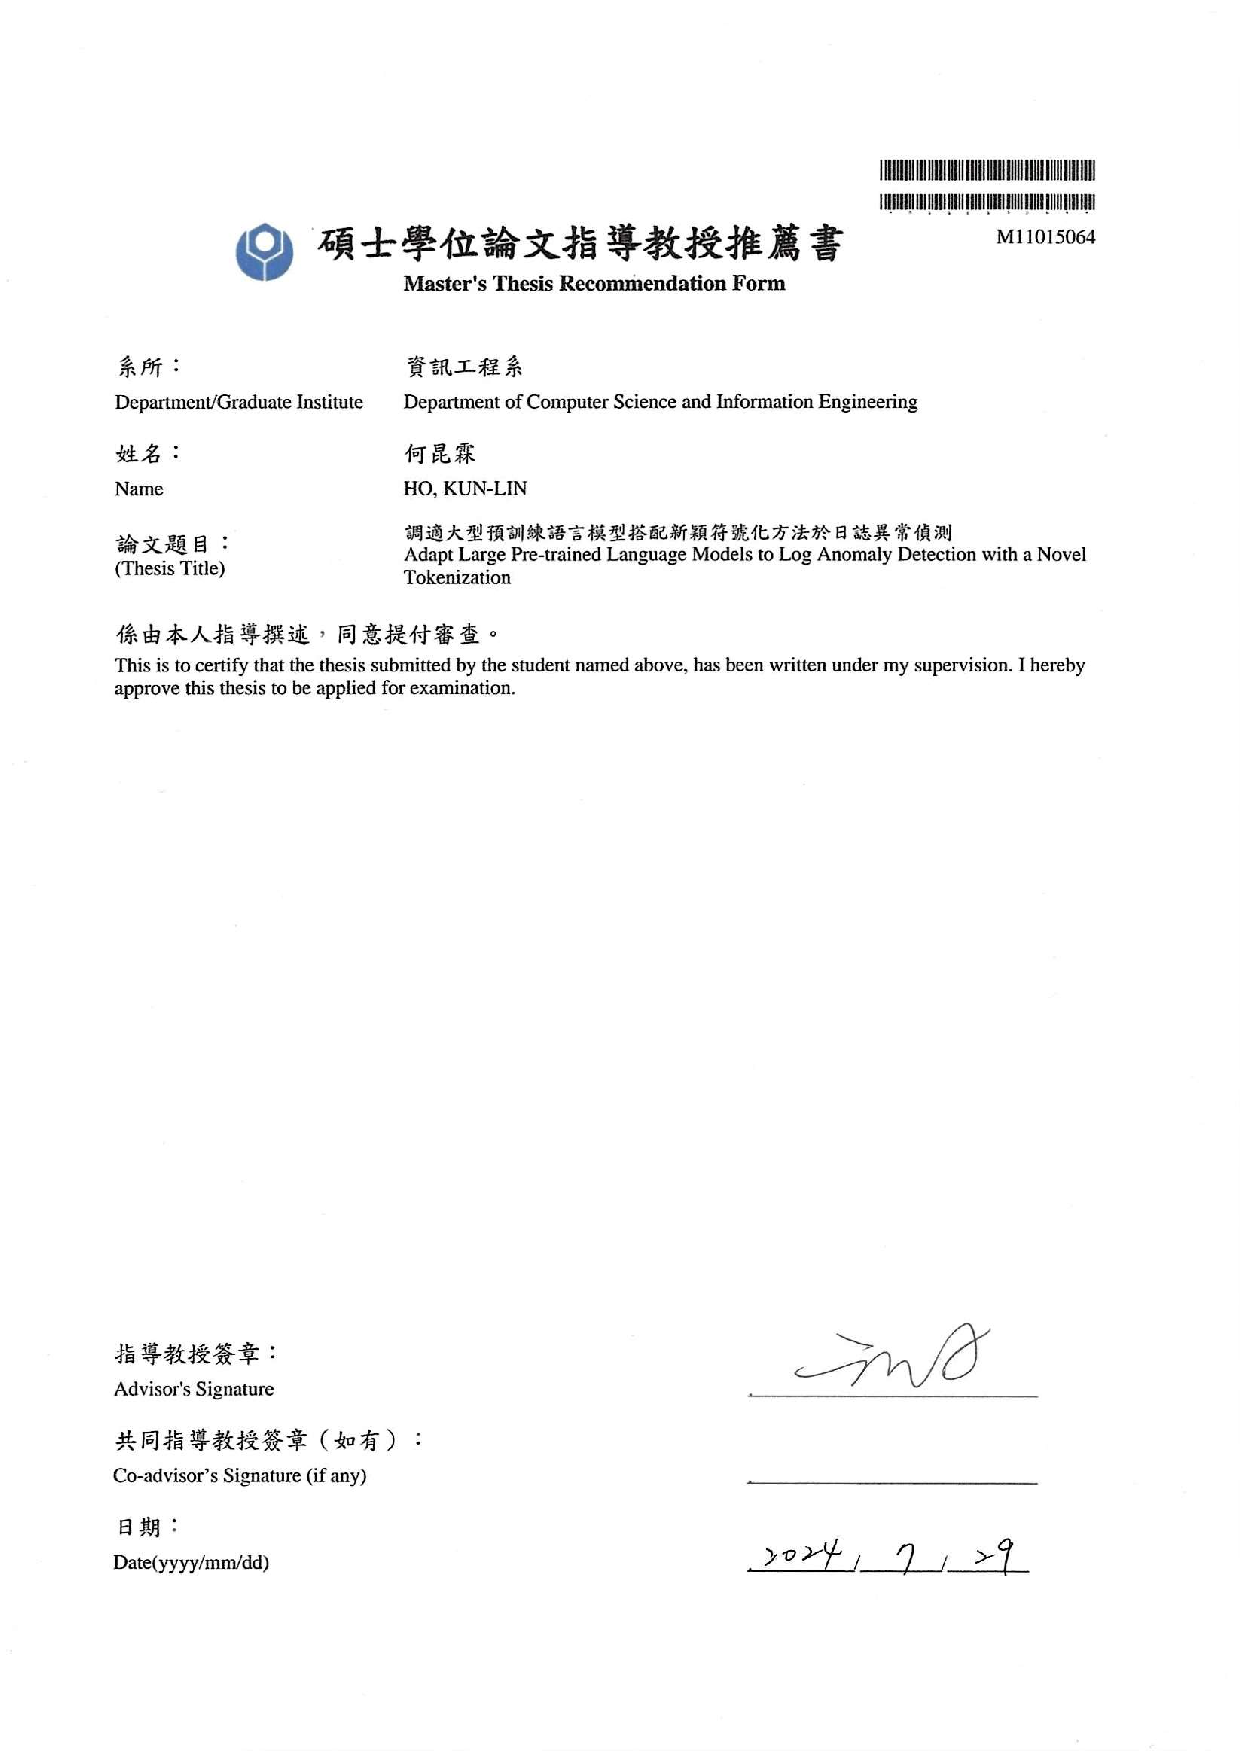
\includepdf[pages=-]{000_frontpages/01_recommendation_form.pdf}
%\newpage

% 判斷是否要浮水印？
\ifx\mywatermark\undefined 
  \thispagestyle{empty}  % 無頁碼、無 header (無浮水印)
\else
  \thispagestyle{EmptyWaterMarkPage} % 無頁碼、有浮水印
\fi

%%%%%%%%%%%%%%%%%%%%%%%%%%%%%%%%%%%%%%%%%%%%%%%%%%%%%%%%%%
%       論文口試委員審定書 Qualification Form
%%%%%%%%%%%%%%%%%%%%%%%%%%%%%%%%%%%%%%%%%%%%%%%%%%%%%%%%%%
%
% insert the printed standard form when the thesis is ready to bind
% 在口試完成後，再將已簽名的審定書放入以便裝訂
% create an entry in table of contents for 審定書
% 目前送出空白頁
% \newpage{\thispagestyle{empty}\addcontentsline{toc}{chapter}{\nameCommitteeForm}\mbox{}\clearpage}
\addcontentsline{toc}{chapter}{\nameCommitteeForm}
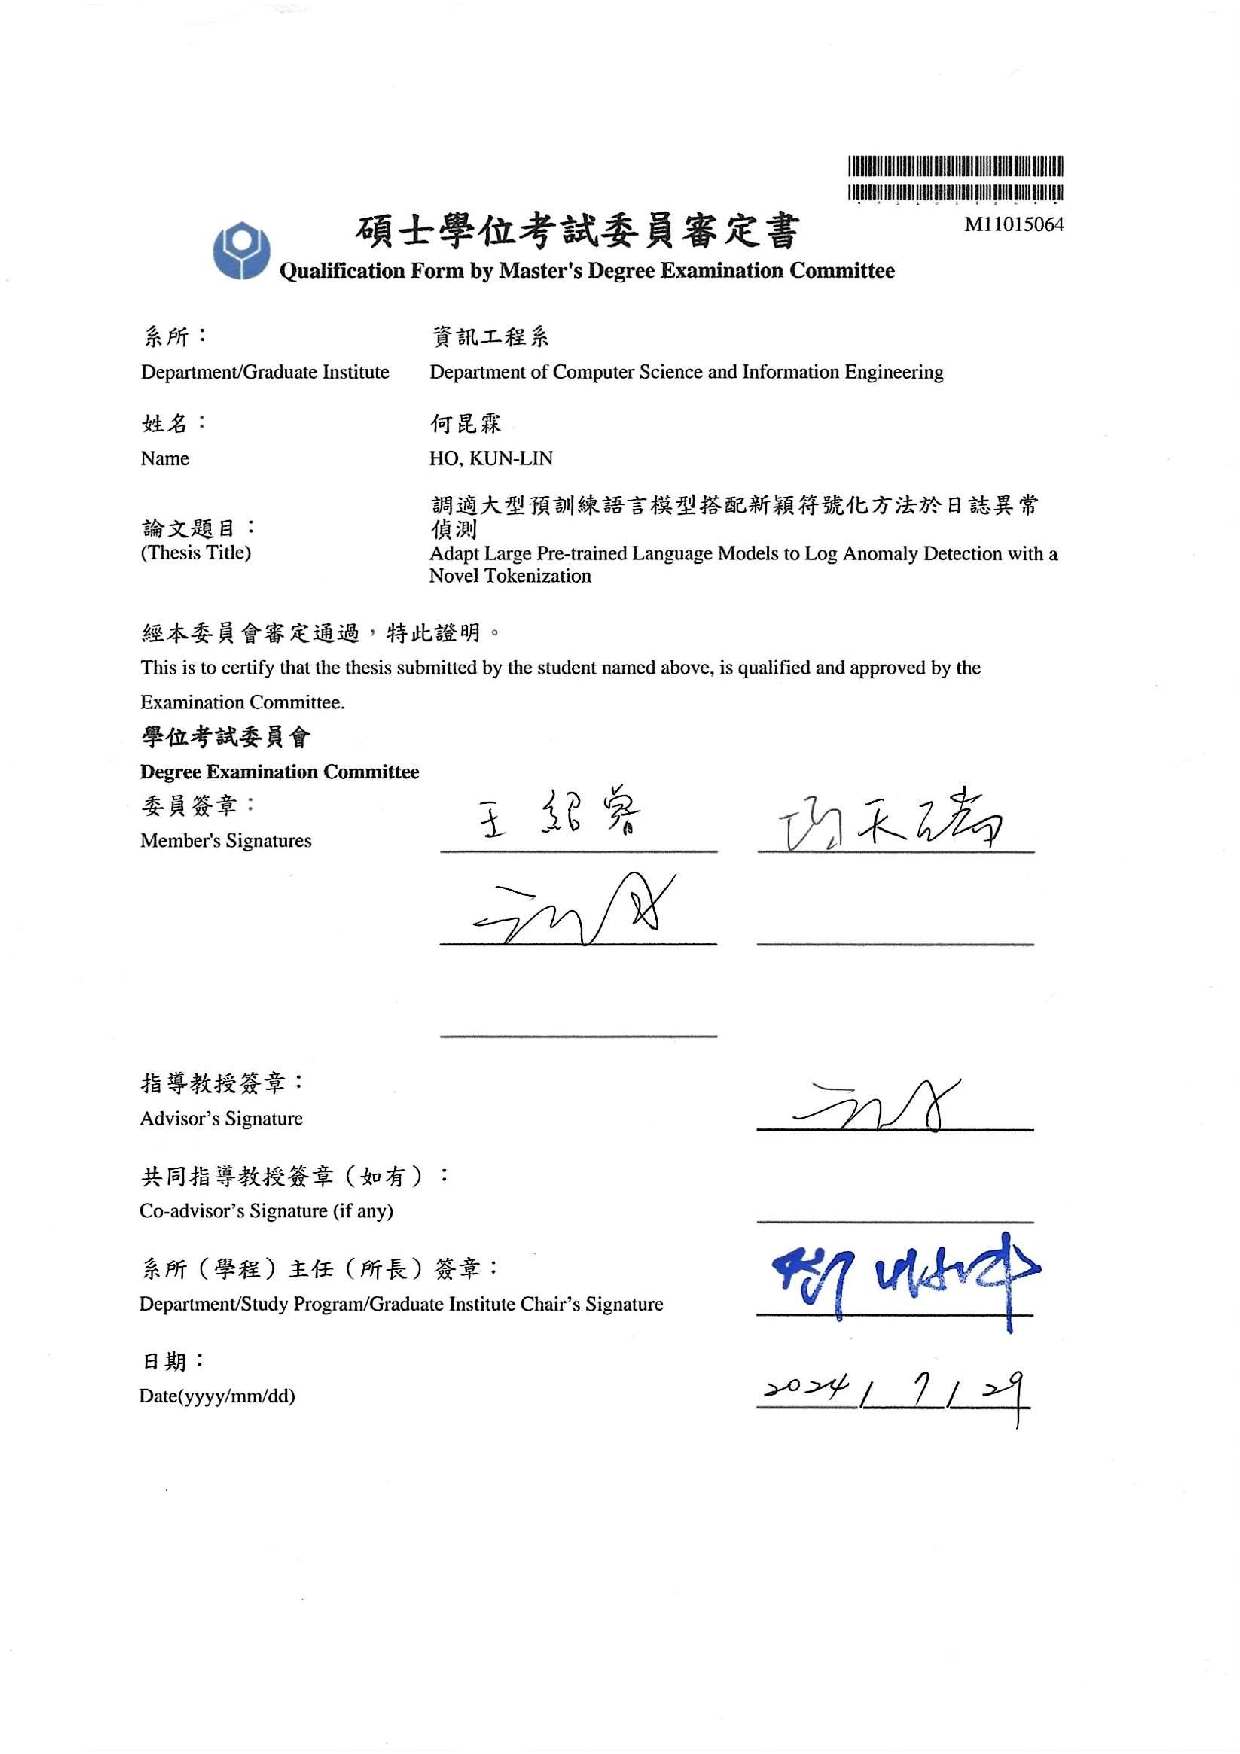
\includepdf[pages=-]{000_frontpages/02_qualification_form.pdf}


%%%%%%%%%%%%%%%%%%%%%%%%%%%%%%%%%%%%%%%%%%%%%%%%%%%%%%%%%%
%              中文摘要 Chinese Abstract
%%%%%%%%%%%%%%%%%%%%%%%%%%%%%%%%%%%%%%%%%%%%%%%%%%%%%%%%%%

\newpage
\thispagestyle{plain}  % 無 header，但在浮水印模式下會有浮水印
% create an entry in table of contents for 中文摘要
\addcontentsline{toc}{chapter}{\nameCabstract}

% aligned to the center of the page
\begin{center}
% font size (relative to 12 pt):
% \large (14pt) < \Large (18pt) < \LARGE (20pt) < \huge (24pt)< \Huge (24 pt)
% Set the line spacing to single for the names (to compress the lines)
\renewcommand{\baselinestretch}{1}   %行距 1 倍
% it needs a font size changing command to be effective
\makebox[.2\linewidth][s]{\Large{摘要}}\\
\end{center}
% Resume the line spacing to the desired setting
\renewcommand{\baselinestretch}{\mybaselinestretch}   %恢復原設定
%it needs a font size changing command to be effective
% restore the font size to normal
\normalsize
%%%%%%%%%%%%%
{\renewcommand{\baselinestretch}{1.2}\normalsize
大型視覺語言模型（Vision-Language Models，VLMs）在多模態任務上表現卓越，但高度依賴雲端基礎設施與高效能 GPU，難以直接部署於資源受限的邊緣環境。本論文針對記憶體低於 800 MB、純 CPU 推理、延遲低於 10 毫秒及任務關鍵場景零幻覺容忍等嚴苛約束，開發適用於裝置端部署的輕量視覺語言模型。

本論文提出兩套系統。\textbf{BitMar} 為 1400 萬參數、採用 1.58 位元三元量化的多模態模型，整合跨模態融合管線與外部情節記憶矩陣（512 槽位，128 維）。啟用情節記憶後，推理吞吐量提升約 7.5 倍，能耗降低 79\%，並在實體追蹤、組合推理及視覺問答任務上獲得 3 至 4 個百分點的準確率提升，驗證了極限量化、跨模態融合與情節記憶在同一架構中共存的可行性。\textbf{EmberVLM} 為本論文主要貢獻，總計 1.64 億參數（4000 萬可訓練），採用四階段課程式訓練策略。其情節記憶模組採用高斯距離定址與新穎性觸發動態寫入機制，每步推理僅增加 1.2 MB 記憶體佔用及不足 3\% 的浮點運算量，可將機器人選擇任務之巨集 F1 分數從 0.035 提升至 0.297。其視覺缺失精煉器（VA Refiner）為免訓練的幻覺抑制機制，透過雙視角邏輯差異分析與解碼器中間層神經元激活監控，無需額外前向傳遞即可抑制視覺上無依據的輸出。

EmberVLM 在三項任務關鍵基準上取得最佳成績：Top-N 機器人選擇（巨集 F1 = 0.42）、緊急視覺辨識（準確率 0.64）及地理災害理解（準確率 0.72）。完整推理堆疊在純 CPU 裝置上僅需 5.22 毫秒，記憶體佔用低於 800 MB。VA 精煉器將對抗性幻覺率從 29\% 降至 22\%。全訓練週期碳排放實測為 25.3 kg CO$_2$eq，展示了任務關鍵邊緣人工智慧的永續訓練路徑。

\chinesekeywords{邊緣人工智慧、視覺語言模型、情節記憶、幻覺抑制、模型量化、資源受限部署}
}


%%%%%%%%%%%%%%%%%%%%%%%%%%%%%%%%%%%%%%%%%%%%%%%%%%%%%%%%%%
%              英文摘要 English Abstract
%%%%%%%%%%%%%%%%%%%%%%%%%%%%%%%%%%%%%%%%%%%%%%%%%%%%%%%%%%

\newpage
%\thispagestyle{plain}  % 無 header，但在浮水印模式下會有浮水印
\chapter*{\protect\makebox{Abstract}}
% create an entry in table of contents for 英文摘要
\addcontentsline{toc}{chapter}{\nameEabstract}

{\renewcommand{\baselinestretch}{1.2}\normalsize
Large vision-language models (VLMs) achieve strong multimodal performance but depend entirely on cloud infrastructure and high-end GPU hardware, making them unsuitable for resource-constrained, offline, and privacy-sensitive deployment scenarios. This thesis develops compact VLMs for on-device inference under simultaneous hard constraints: under 800~MB RAM, CPU-only execution, sub-10~ms latency, and zero tolerance for hallucinated outputs in mission-critical settings.

Two systems are presented. \textbf{BitMar} is a 14M-parameter, 1.58-bit ternary-quantized multimodal model integrating a cross-modal fusion pipeline with an external episodic memory matrix (512 slots, 128 dimensions). Enabling episodic memory yields approximately $7.5\times$ throughput improvement and 79\% energy reduction over the memory-free baseline, alongside 3--4 percentage-point accuracy gains on entity tracking, compositional reasoning, and visual question answering. BitMar establishes the foundational compatibility of extreme quantization, cross-modal fusion, and episodic memory in a single architecture. \textbf{EmberVLM} is the primary contribution: a 164M-parameter VLM (40M trainable) with a four-stage training curriculum. Its Episodic Memory Module employs Gaussian distance-based addressing and novelty-triggered online writes, adding only 1.2~MB RAM and under 3\% extra FLOPs per inference step, boosting robot-selection Macro-F1 from 0.035 to 0.297. Its Visual Absence (VA) Refiner is a training-free hallucination control mechanism fusing logit-space dual-view consistency with neuron-level mid-decoder activation monitoring, requiring no additional forward passes.

EmberVLM achieves the best reported results among sub-billion-parameter models on three mission-critical benchmarks: Top-N Robot Selection (Macro-F1~=~0.42), emergency visual recognition (Accuracy~=~0.64), and geospatial disaster understanding (Accuracy~=~0.72). The full inference stack runs at 5.22~ms per sample on a CPU-only device with under 800~MB RAM. The VA Refiner reduces adversarial hallucination rate from 29\% to 22\%. Total measured training emissions are 25.3~kg~CO$_2$eq, demonstrating that mission-critical multimodal AI can be trained sustainably.

\keywords{Edge AI, Vision-Language Models, Episodic Memory, Hallucination Mitigation, Model Quantization, Resource-Constrained Deployment}
}


%%%%%%%%%%%%%%%%%%%%%%%%%%%%%%%%%%%%%%%%%%%%%%%%%%%%%%%%%%
%                誌謝 Acknowledgements
%%%%%%%%%%%%%%%%%%%%%%%%%%%%%%%%%%%%%%%%%%%%%%%%%%%%%%%%%%
%
% Acknowledgment
\newpage
\chapter*{\protect\makebox{\nameAckn}} %\makebox{} is fragile; need protect
\addcontentsline{toc}{chapter}{\nameAckn}
% TODO: Student to fill in acknowledgements



%%%%%%%%%%%%%%%%%%%%%%%%%%%%%%%%%%%%%%%%%%%%%%%%%%%%%%%%%%
%         目錄 Table of Contents (auto generated)
%%%%%%%%%%%%%%%%%%%%%%%%%%%%%%%%%%%%%%%%%%%%%%%%%%%%%%%%%%
%
% Table of contents
\newpage
\renewcommand{\contentsname}{\protect\makebox{\nameToc}}
%\makebox{} is fragile; need protect
\addcontentsline{toc}{chapter}{\nameToc}
\tableofcontents

%%%%%%%%%%%%%%%%%%%%%%%%%%%%%%%
%       圖目錄 
%%%%%%%%%%%%%%%%%%%%%%%%%%%%%%%
%
% List of Figures
\newpage
\renewcommand{\listfigurename}{\protect\makebox{\nameTof}}
%\makebox{} is fragile; need protect
\addcontentsline{toc}{chapter}{\nameTof}
\listoffigures

%%%%%%%%%%%%%%%%%%%%%%%%%%%%%%%
%       表目錄 
%%%%%%%%%%%%%%%%%%%%%%%%%%%%%%%
%
% List of Tables
\newpage
\renewcommand{\listtablename}{\protect\makebox{\nameLot}}
%\makebox{} is fragile; need protect
\addcontentsline{toc}{chapter}{\nameLot}
\listoftables

%%%%%%%%%%%%%%%%%%%%%%%%%%%%%%%
%       演算法目錄 
%%%%%%%%%%%%%%%%%%%%%%%%%%%%%%%
%
% List of Figures
\newpage
\renewcommand{\listalgorithmname}{\protect\makebox{\nameToa}}
%\makebox{} is fragile; need protect
\addcontentsline{toc}{chapter}{\nameToa}
\listofalgorithms

\newpage
%% 論文本體頁碼回復為阿拉伯數字計頁，並從頭起算
\pagenumbering{arabic}
%%%%%%%%%%%%%%%%%%%%%%%%%%%%%%%% 




	%----------------------------------------------------------------------------------------------------------------------------------------------------------
	% main body 論文主體。建議以「章」為檔案分割的依據。
	% 以下為建議的命名分類
	%   introduction.tex   related_work.tex  protocol.tex  evaluation.tex  conclusion.tex
	% 做為這幾個「章」的檔案名稱，並將檔案存放於資料夾 sections/ 下
	% 實際命名方式可以隨你意
	% 在撰寫各章草稿時，可以把其他章節關掉 (行首加百分號)
	% \input{example/example_body.tex}  % 所附的範例

        \chapter{Introduction}
\label{cha:intro}

\section{Background and Motivation}
\label{sec:intro_background}

Vision-Language Models (VLMs) represent one of the most transformative advances in modern artificial intelligence, enabling systems to jointly reason over visual and textual information for tasks including image captioning, visual question answering, scene understanding, and multimodal dialogue. Landmark architectures such as Flamingo~\cite{alayrac2022flamingo}, BLIP-2~\cite{li2023blip2}, GPT-4V~\cite{openai2023gpt4}, and Gemini~\cite{team2023gemini} have demonstrated that scaling model parameters alongside multimodal pretraining yields qualitative improvements in cross-modal grounding and generation. This scaling trend has continued unabated, with frontier VLMs now exceeding hundreds of billions of parameters.

However, this impressive progress carries a critical structural dependency: virtually all state-of-the-art VLMs are designed for and evaluated in \emph{cloud-hosted} settings. They assume access to GPU clusters, high-bandwidth internet connectivity, centralized storage, and milliseconds-to-seconds latency budgets that are acceptable only when a remote server handles inference. This assumption is so deeply embedded in the design of modern VLMs that it is rarely articulated as a limitation, yet it categorically excludes an important and growing class of real-world deployment scenarios.

Consider the following concrete deployment contexts:
\begin{itemize}
    \item \textbf{Disaster response robotics.} Following earthquakes, floods, or structural collapses, autonomous robots must navigate rubble, classify environments, and select appropriate robotic assets for deployment. Network infrastructure is typically destroyed, and round-trip latency to a cloud server is unacceptable when a robot is making split-second decisions in a life-critical zone.
    \item \textbf{Aerial surveillance drones.} Unmanned aerial vehicles conducting reconnaissance or border monitoring in remote terrain operate beyond cellular or satellite connectivity windows. They must perform real-time scene classification and anomaly detection entirely on-device.
    \item \textbf{Autonomous vehicles.} Road safety systems require sub-50ms visual reasoning to detect obstacles, pedestrians, and road conditions. Transmitting raw sensor data to a cloud server and waiting for a response is physically impossible at highway speeds.
    \item \textbf{Industrial inspection.} Facilities handling hazardous materials or electromagnetic-sensitive equipment frequently operate in radio-frequency-silent zones. Visual inspection AI must run locally on embedded hardware.
    \item \textbf{Medical edge devices.} Point-of-care diagnostic devices in low-resource clinical settings lack reliable internet and must perform visual analysis (e.g., dermatological screening, wound assessment) on battery-powered hardware.
\end{itemize}

All of these scenarios impose hard, simultaneous constraints: limited VRAM or SRAM (often under 1~GB), CPU-only inference (no discrete GPU), zero-tolerance for hallucinated outputs in safety-critical decisions, and complete independence from network connectivity. These constraints are not engineering inconveniences to be addressed incrementally; they are categorical requirements that current VLMs cannot meet.

The central challenge of this thesis is therefore not merely ``making models smaller.'' Smaller models have existed for some time (SmolVLM-256M, MobileVLM, LLaVA-Phi), yet none are designed for simultaneous CPU-only inference, sub-10ms latency, under 800~MB RAM, and zero-hallucination tolerance in mission-critical classification tasks. The research gap is this: \textbf{achieving reliable, hallucination-suppressed, contextually aware multimodal reasoning under simultaneous constraints of parameter budget, memory footprint, computational budget, and connectivity independence.}

\section{Research Challenges}
\label{sec:intro_challenges}

This thesis identifies three primary, interconnected challenges that any viable edge VLM must address.

\subsection{Memory and Compute Constraints}
\label{subsec:challenge_compute}

Even sub-billion-parameter VLMs impose memory and latency requirements that exceed the capabilities of commodity edge hardware. SmolVLM-256M, one of the smallest publicly available VLMs, requires a discrete GPU for practical inference and achieves 941~ms per sample even in that configuration. InternVL3-1B requires 1,978~MB VRAM and achieves 1,566~ms per sample on the target CPU-only deployment hardware used in this thesis (AMD Ryzen 3 4100). These numbers are not competitive for real-time edge deployment where latency budgets are in the tens of milliseconds and no discrete GPU is available.

The fundamental technical mismatch arises from the full-precision floating-point arithmetic and large activation tensors that current VLMs require, combined with transformer attention complexity that scales quadratically with sequence length. Even architectures specifically marketed as ``efficient'' have not been designed for the specific combination of CPU-only inference, sub-800~MB RAM, and sub-10ms latency that defines practical edge deployment.

\subsection[Hallucination at the Edge]{Hallucination in Mission-Critical Settings}
\label{subsec:challenge_hallucination}

Hallucination, the generation of tokens unsupported by visual evidence in the input image, is a fundamental and well-documented failure mode in all current VLMs. A model may confidently describe an object that is absent from the image, or assign incorrect attributes to present objects, purely by relying on statistical language priors from pretraining.

In cloud-based consumer applications, hallucination is a quality issue. In mission-critical edge settings, it is a safety failure. If a robot selection system hallucinates the presence of a ``Drone'' when the scene actually shows a flooded corridor requiring an ``Underwater Robot,'' the wrong asset is deployed and the mission fails. If an emergency recognition system hallucinates that a burning structure is a ``normal building,'' emergency response resources are not dispatched.

Existing hallucination mitigation strategies are largely infeasible at the edge. Methods based on grounding supervision or retraining require annotated data and compute that are not available during deployment. Visual Contrastive Decoding (VCD)~\cite{leng2024vcd}, while effective, requires an extra forward pass with perturbed visual input, doubling inference cost, which is unacceptable at the latency budgets required. What is needed is a training-free, zero-extra-forward-pass mechanism that operates within the model's existing inference graph.

\subsection{Knowledge Staleness and Distributional Shift}
\label{subsec:challenge_staleness}

Edge VLMs are typically frozen after deployment: their parametric weights do not change in the field. Yet the environments they encounter are dynamic and may differ substantially from the training distribution. Novel robot morphologies, previously unseen disaster scenarios, or unfamiliar terrain types may appear after deployment.

Without a mechanism for incorporating new contextual knowledge, models collapse under distributional shift. This is starkly demonstrated by the EmberVLM NoMemory baseline evaluated in this thesis: without episodic memory conditioning, the model degrades into a near single-class predictor on the robot selection task, achieving validation accuracy of 0.097 and macro-F1 of 0.035. It over-indexes on the most frequent class while entirely failing on minority classes. The episodic memory mechanism must therefore be more than a retrieval cache: it must provide a principled way to accumulate new deployment-time knowledge without catastrophic forgetting, without retraining, and without violating the memory budget of the target hardware.

\section{Research Overview and Contributions}
\label{sec:intro_contributions}

This thesis presents a unified research trajectory toward addressing these three challenges simultaneously, structured around two complementary research contributions.

\paragraph{BitMar.}
BitMar~\cite{aman2025bitmar} is the first published contribution of this thesis research. BitMar is a 14M-parameter, 1.58-bit ternary-quantized multimodal model that establishes the foundational proof-of-concept for the thesis. It demonstrates that (i) aggressive ternary quantization ({$-$1, 0, +1} weights at 1.58 bits/parameter) is compatible with cross-modal multimodal fusion, (ii) an external episodic memory module provides measurable efficiency and accuracy benefits in the quantized multimodal setting, and (iii) the combination of quantization, cross-modal fusion, and episodic memory can co-exist in a 14M-parameter architecture. BitMar validated the core thesis proposition before the larger EmberVLM system was built.

\paragraph{EmberVLM.}
EmberVLM is the primary architectural contribution of this thesis. It is a 164M total parameter (40M trainable) tiny VLM purpose-built for mission-critical edge deployment. EmberVLM introduces two novel modules: an Episodic Memory Module with scope detection, Gaussian-addressed retrieval, novelty-triggered online writes, and knowledge consolidation distillation; and a Visual Absence (VA) Refiner combining logit-space dual-view consistency with neuron-level mid-decoder activation monitoring. EmberVLM achieves the best reported performance among sub-billion-parameter models on three mission-critical benchmarks, at 5.22~ms per sample on CPU-only hardware with under 800~MB RAM.

The specific contributions of this thesis are:

\begin{enumerate}
    \item \textbf{BitMar}: The first architecture to jointly integrate 1.58-bit multimodal encoding with an external episodic memory for edge deployment. BitMar achieves approximately $7.5\times$ throughput improvement and 79\% energy reduction versus the memory-free baseline, delivering 3--4 percentage-point gains on entity tracking, compositional reasoning, and visual question answering at 14M parameters.

    \item \textbf{EmberVLM architecture}: A tiny VLM (164M total parameters, 40M trainable) employing a four-stage training curriculum (visual-language alignment, multimodal instruction tuning, task adaptation, and latent chain-of-thought integration), achieving competitive mission-critical performance against models $5\text{--}10\times$ larger.

    \item \textbf{Episodic Memory Module}: A dynamically loadable memory system with fixed overhead (1.2~MB RAM, $<$3\% extra FLOPs per inference step), a lightweight scope detector, Gaussian distance-based addressing, novelty-triggered online writes with a hybrid LRU-LFU eviction policy, and an optional Stage~5 knowledge consolidation distillation phase. The module boosts robot-selection macro-F1 from 0.035 to 0.297.

    \item \textbf{Visual Absence (VA) Refiner}: A training-free plug-in hallucination control mechanism fusing dual-view logit discrepancy with neuron-level mid-decoder activation monitoring (layers 10--14 of SmolLM-135M), applied via type-aware thresholds and temporal burst detection. The VA Refiner reduces POPE Adversarial hallucination rate from 29\% to 22\%, an absolute reduction of 7 percentage points.

    \item \textbf{Comprehensive mission-critical evaluation}: State-of-the-art results for sub-billion-parameter models on Top-N Robot Selection (Macro-F1~=~0.42), VERI-Emergency (Accuracy~=~0.64), and GEO-Bench-VLM (Accuracy~=~0.72); inference at 5.22~ms per sample on CPU-only hardware with $<$800~MB RAM; total measured training emissions of 25.3~kg~CO$_2$eq.
\end{enumerate}

\section{Thesis Organization}
\label{sec:intro_organization}

The remainder of this thesis is structured as follows.

Chapter~\ref{cha:related} surveys related work across five areas: tiny and edge-deployable VLMs, model quantization, episodic memory in language and multimodal systems, hallucination detection and control, and mission-critical visual recognition benchmarks.

Chapter~\ref{cha:bitmar} presents BitMar in full detail, including its architecture, training objectives, dataset, and experimental results. This chapter also identifies the open questions that motivated the design of EmberVLM.

Chapter~\ref{cha:embervlm} presents the EmberVLM architecture, covering the base multimodal pipeline, the Episodic Memory Module, the Visual Absence Refiner, and the four-stage training curriculum. Chapter~\ref{cha:experiments} presents experimental results for both BitMar and EmberVLM, including mission-critical benchmark evaluations, ablation studies, edge deployment latency, and mechanistic interpretability of hallucinations.

Chapter~\ref{cha:discussion} synthesizes findings across both works, discussing the research progression from BitMar to EmberVLM, the empirical case for episodic memory at the edge, hallucination as a systems-level problem, and implications for sustainable AI development.

Chapter~\ref{cha:conclusion} concludes the thesis and outlines directions for future research.

Section~\ref{sec:bitmar_impl} in Chapter~\ref{cha:bitmar} provides complete hyperparameter tables, corpus statistics, and preprocessing details for BitMar. Section~\ref{sec:embervlm_carbon} in Chapter~\ref{cha:embervlm} provides the full architectural specification and carbon tracking methodology for EmberVLM.

        \chapter{Related Work}
\label{cha:related}

This chapter surveys prior work across five research areas directly relevant to the contributions of this thesis: tiny and edge-deployable vision-language models, model quantization for efficient inference, episodic memory in language and multimodal systems, hallucination detection and control in VLMs, and mission-critical visual recognition benchmarks. Each section contextualizes prior work relative to the thesis contributions and concludes with a statement of how this thesis advances beyond the existing literature.

\section[Tiny and Edge-Deployable VLMs]{Tiny and Edge-Deployable Vision-Language Models}
\label{sec:related_tiny_vlm}

The rapid scaling of VLMs has prompted a parallel line of work on compact architectures that preserve multimodal capability under reduced parameter budgets. SmolVLM~\cite{smolvlm2024} demonstrates that sub-billion-parameter models paired with strong vision encoders can achieve competitive results on standard benchmarks while being deployable on commodity hardware. The authors show that careful data curation and efficient vision tokenization significantly impact quality at small scales. However, even SmolVLM-256M requires a discrete GPU for practical inference and does not target CPU-only deployment.

MobileVLM~\cite{chu2023mobilevlm} proposes lightweight vision-language connectors and mobile-optimized language backbones for responsive on-device inference. The architecture demonstrates that the vision-language bridge is a critical bottleneck in compact VLMs, and that lightweight depthwise-separable designs can reduce parameter count. MobileVLM V2~\cite{chu2024mobilevlmv2} extends this with token compression and improved throughput. While these models represent genuine progress, they target GPU-based mobile devices rather than the CPU-only, RAM-limited deployments addressed in this thesis.

LLaVA-Phi~\cite{zhu2024llavaphi} combines a compact Phi-2 language model with a CLIP vision encoder, showing that 2.7B-parameter instruction-tuned VLMs can approach much larger models at substantially lower inference cost. This is relevant to robotics and edge deployment, but 2.7B parameters still exceeds the practical limits of the target hardware by more than an order of magnitude. TinyGPT-V~\cite{yuan2024tinygptv} further reduces parameters by employing efficient patch embedding strategies and distillation from larger teacher models. MiniCPM-V~\cite{hu2024minicpmv} pursues efficiency through selective parameter sharing and dynamic token pruning, achieving strong results in the 2--3B parameter range. H2OVL-Mississippi targets inference on low-resource hardware by combining aggressive pruning with knowledge distillation.

The consistent pattern across all prior compact VLM work is that none simultaneously targets CPU-only inference, under 800~MB RAM, sub-10ms per-sample latency, and zero-hallucination reliability for mission-critical classification. Most assume GPU acceleration; all treat hallucination control and epistemic memory as orthogonal concerns rather than core design requirements. This thesis addresses the full intersection of these requirements with a unified architecture.

\section{Model Quantization for Efficient Inference}
\label{sec:related_quant}

Quantization reduces model memory and compute requirements by representing weights and/or activations at lower bit-widths than standard 32-bit floating point. BitNet~\cite{wang2023bitnet} demonstrates that transformer language models can be trained from scratch with 1-bit weights without catastrophic accuracy degradation, enabling highly memory-efficient inference on specialized hardware. The key insight is that signed integer multiply-accumulate operations can replace expensive floating-point operations throughout the forward pass.

BitNet~b1.58~\cite{ma2024bitnet158} extends this to ternary weights $\{-1, 0, +1\}$, which require only 1.58 bits per parameter (the binary entropy of a ternary distribution). At this precision, nearly all multiply operations can be replaced by additions and subtractions, dramatically reducing compute on hardware without dedicated low-precision units. BitNet~b1.58 achieves near-lossless perplexity compared to full-precision baselines when trained at sufficient scale, validating ternary quantization as a practical compression strategy.

GPTQ~\cite{frantar2022gptq} provides one-shot post-training quantization via approximate second-order information, enabling efficient 3--4 bit quantization of already-trained large models without backpropagation. This is complementary to BitNet-style native quantization and is widely used to compress pre-trained models for deployment. AWQ~\cite{lin2023awq} proposes activation-aware weight quantization that identifies and protects salient channels most sensitive to quantization error, achieving strong 4-bit compression across language and multimodal models.

BitMar, the first contribution of this thesis, applies 1.58-bit ternary quantization to a multimodal pipeline: both the text encoder and all downstream fusion, memory, and decoder projections operate under ternary weight constraints. This is a direct extension of BitNet~b1.58's quantization scheme to the cross-modal setting, and to the best of our knowledge is the first architecture to demonstrate that ternary quantization is compatible with cross-modal attention fusion and episodic memory conditioning simultaneously.

\section[Episodic Memory in Neural Models]{Episodic Memory in Language and Multimodal Models}
\label{sec:related_memory}

The idea of augmenting neural networks with external, addressable memory has a long history. Differentiable Neural Computers (DNC)~\cite{graves2016dnc} introduced the first complete architecture for learning explicit read and write operations over an external memory matrix, demonstrating that neural networks can solve complex algorithmic tasks requiring long-range structured recall. While DNCs operate only on symbolic sequences, they established the key design principles, including content-based addressing, soft writes, and read-weight computation, that inform modern memory-augmented VLMs.

Memorizing Transformers~\cite{wu2022memorising} show that augmenting standard transformer language models with external memory lookups over past key-value pairs improves long-context modeling without changing core model weights. This work demonstrates that memory retrieval can be separated from parametric knowledge, allowing a frozen model to leverage growing context stores. Retrieval-Augmented Generation (RAG)~\cite{lewis2020rag} takes a related approach, connecting generative models to large external document stores to improve factuality and reduce hallucination on knowledge-intensive tasks. However, RAG targets server-scale infrastructure: dense passage retrieval from millions of documents requires GPU-accelerated vector search engines that are impractical at the edge.

Larimar~\cite{das2024larimar} presents a memory-controlled LLM framework in which episodes are written to and retrieved from a structured store using a differentiable interface, enabling the model to update its knowledge without full retraining. This is conceptually close to the EmberVLM episodic memory design, though Larimar targets large language models on GPU servers rather than tiny VLMs on CPU-only edge hardware.

EGO and related selective episodic memory strategies explore how memory writes can be conditioned on novelty signals to prevent the memory matrix from being overwritten with redundant common experiences. This informs EmberVLM's novelty-triggered write mechanism, where a minimum-distance novelty score gates whether an incoming embedding warrants a new memory write.

A critical distinction between the memory systems in this thesis and server-scale RAG or database-backed retrieval: both BitMar and EmberVLM use \emph{fixed-size, on-device episodic matrices} that fit entirely within the primary compute device's RAM (1.2~MB). No external database query, network request, or dense retrieval index is involved. Memory reads and writes are pure matrix operations that complete in microseconds. This makes the memory system viable for real-time edge inference in a way that server-scale retrieval is not.

\section{Hallucination Detection and Control in VLMs}
\label{sec:related_hallucination}

Hallucination in VLMs, the generation of tokens unsupported by the input image, has been extensively documented and benchmarked. Rohrbach~et~al.~\cite{rohrbach2018hallucination} showed that image captioning models systematically generate statistically likely but visually absent objects, even in high-performing systems. They demonstrate that hallucination correlates with co-occurrence statistics in training data rather than actual visual evidence. This foundational finding motivates all subsequent hallucination mitigation research.

The POPE benchmark~\cite{li2023pope} formalizes object hallucination evaluation as a polling-based yes/no question protocol: given an image, models are asked whether specific objects are present. POPE includes adversarial splits where absent objects are specifically chosen to have high co-occurrence with genuinely present objects, making them maximally likely to be hallucinated. POPE has become the standard evaluation for object-level hallucination across the VLM literature.

Visual Contrastive Decoding (VCD)~\cite{leng2024vcd} addresses hallucination without retraining by contrasting output distributions from original and spatially distorted visual inputs. Tokens whose generation probability is not significantly affected by the visual content are penalized, encouraging the model to rely on actual image features rather than language priors. VCD is effective across multiple large VLM families, but it requires a complete second forward pass with perturbed input, doubling the inference cost. For the CPU-only, sub-10ms deployment targets of this thesis, this overhead is unacceptable.

Instruction-following calibration approaches train models to express uncertainty when visual evidence is insufficient, requiring either additional labeled data or specialized fine-tuning pipelines. Grounding supervision methods add explicit visual localization objectives during training to reduce the gap between language-prior generation and visually evidenced generation. Both classes of methods require retraining or supplementary annotation, making them infeasible for deployment-time use on frozen edge models.

The Visual Absence (VA) Refiner introduced in this thesis occupies a previously unexplored position in the mitigation landscape: it is training-free, requires no extra forward passes, needs no labeled grounding data, and operates by monitoring the model's own internal neuron-level activation patterns during a single standard forward pass. By hooking into mid-decoder FFN layers (10--14 of SmolLM-135M), the VA Refiner detects the characteristic activation signature of hallucinated tokens, specifically symmetric patterns that do not change when the visual input is removed, and applies type-aware logit penalties to suppress them. This mechanistic grounding distinguishes the VA Refiner from all prior approaches and makes it uniquely suitable for frozen edge deployment.

\section{Mission-Critical Visual Recognition Benchmarks}
\label{sec:related_benchmarks}

Standard VLM benchmarks such as VQA v2~\cite{VQA}, GQA~\cite{hudson2019gqa}, and SugarCrepe~\cite{hsieh2023sugarcrepe} are designed to measure general visual question answering and compositional reasoning capabilities across diverse image domains. While valuable for comparative evaluation, these benchmarks do not capture the reliability requirements of safety-critical deployment. A model that achieves high GQA accuracy may still produce catastrophically wrong outputs in emergency or disaster scenarios.

The Top-N Robot Selection task, used as the primary evaluation in this thesis, is a multi-label morphology classification problem: given a scene image and mission description, predict which robot types (Drone, Underwater Robot, Humanoid, Wheeled, Legged) should be deployed. This task is mission-critical because wrong predictions directly lead to incorrect asset allocation in emergency response scenarios.

VERI-Emergency~\cite{choi2026better}, introduced at WACV 2026, is a visual emergency recognition benchmark covering fire, flooding, chemical hazards, and related emergency scenarios. It introduces an asymmetric evaluation metric structure distinguishing OverRx (false positive rate: wrongly flagging non-emergencies) from UnderRx (false negative rate: missing genuine emergency signals). For safety-critical deployment, UnderRx is the more consequential metric: a missed emergency is more dangerous than a false alarm.

GEO-Bench-VLM~\cite{danish2025geobench}, introduced at ICCV 2025, is a geospatial disaster understanding benchmark covering satellite and aerial imagery of flood zones, wildfire damage, earthquake devastation, and infrastructure collapse. It evaluates models on fine-grained scene classification tasks requiring both visual recognition and geographical contextual reasoning.

Together, these three benchmarks provide a more realistic and demanding evaluation surface for edge-deployable VLMs than standard generative benchmarks. EmberVLM achieves state-of-the-art performance across all three among sub-billion-parameter models, while simultaneously meeting strict edge-deployment latency and memory constraints.

\section{Low-Carbon and Sustainable AI}
\label{sec:related_carbon}

The environmental cost of training large AI models has attracted increasing attention. Strubell~et~al.~\cite{strubell2019energy} estimated that training a large NLP model from scratch produces carbon emissions comparable to five automobile lifetimes. More recent estimates place the training carbon footprint of GPT-3 at approximately 552 tonnes CO$_2$eq~\cite{patterson2021carbon}. As VLMs grow to hundreds of billions of parameters, their environmental impact grows correspondingly.

Compact, parameter-efficient model design is therefore not only a systems engineering concern but an environmental imperative. By constraining total trainable parameters to under 40M and completing all training stages on a dual-A100 setup in approximately 90 hours, EmberVLM achieves a total measured training footprint of 25.3~kg CO$_2$eq, verified using the CodeCarbon~\cite{codecarbon} framework. This is more than 21,000 times smaller than GPT-3's estimated footprint, demonstrating that mission-critical capable multimodal AI can be trained sustainably. This thesis treats low-carbon training not as a secondary benefit but as a primary design constraint.

        \chapter{BitMar: Low-Bit Multimodal Foundation for Edge Deployment}
\label{cha:bitmar}

This chapter presents BitMar~\cite{aman2025bitmar}, the first published contribution of this thesis research. BitMar is framed as a proof-of-concept and foundational work that established key design principles, notably the compatibility of extreme quantization with cross-modal fusion and episodic memory conditioning, which were later refined and scaled in the EmberVLM system (Chapter~\ref{cha:embervlm}).

\section{Motivation and Research Goals}
\label{sec:bitmar_motivation}

The design of BitMar is motivated by a specific question: \emph{Can a model with only 14 million parameters, operating under 1.58-bit ternary weight quantization, achieve meaningful multimodal understanding and generation while incorporating an external episodic memory?}

This question is non-trivial because each component introduces constraints on the others. Quantization reduces the information capacity per parameter, potentially limiting the model's ability to learn fine-grained cross-modal correspondences. Cross-modal fusion requires the text and vision representations to be sufficiently expressive to support accurate attention-based alignment despite the quantization noise. Episodic memory adds a fixed-overhead read/write mechanism that must integrate cleanly with the quantized decoder without introducing instability or gradient conflicts.

\paragraph{Why 1.58-bit?} Ternary weight quantization at 1.58 bits/parameter enables replacing floating-point multiply-accumulate operations with additions and subtractions. A ternary weight $w \in \{-1, 0, +1\}$ applied to activation $a$ gives: $w \cdot a \in \{-a, 0, +a\}$. This means every MHSA and FFN projection can be computed without a single floating-point multiplication, with only conditional negation or zeroing. On hardware without dedicated floating-point units, this is a substantial speedup. Even on standard CPUs, integer arithmetic is significantly faster than floating-point, making ternary quantization the preferred precision for the target edge hardware.

The three design goals for BitMar are:
\begin{enumerate}
    \item \textbf{Unified low-bit multimodal encoding}: both text and vision representation pathways operate under the same 1.58-bit quantization regime, ensuring consistent hardware efficiency across the entire model.
    \item \textbf{Cross-modal fusion under quantization constraints}: the fusion mechanism must preserve semantic alignment between modalities despite ternary weight projections, validated by a contrastive cross-modal alignment objective.
    \item \textbf{External episodic memory without parametric overhead}: the memory system must improve contextual coherence and task accuracy without significantly increasing the trainable parameter count, and must not require any additional inference hardware.
\end{enumerate}

\section{BitMar Architecture Overview}
\label{sec:bitmar_arch}

BitMar follows a four-stage pipeline, illustrated in Figure~\ref{fig:bitmar_arch}:
\begin{enumerate}
    \item \textbf{Parallel low-bit encoders}: A 1.58-bit BitNet-style text encoder and a DiNOv2-based vision encoder (with MLP compression) produce 128-dimensional representations of the input text and image respectively.
    \item \textbf{Cross-modal fusion}: A lightweight cross-attention module (text queries, vision keys/values) fuses the two modalities into a shared 128-dimensional representation.
    \item \textbf{Episodic memory conditioning}: The fused multimodal embedding queries a fixed-size episodic memory matrix ($K{=}512$, $C{=}128$), retrieving a context vector that conditions the decoder.
    \item \textbf{Memory-conditioned autoregressive decoding}: A 1.58-bit BitNet decoder generates text output, with per-layer conditioning from the retrieved memory vector.
\end{enumerate}

All trainable weight matrices in the text encoder, fusion module, and decoder use ternary weights $\{-1, 0, +1\}$ with learned per-layer scales. Activations use 8-bit quantization with per-token max-abs scaling. Softmax, residual connections, and layer normalization operate in FP32 to preserve numerical stability.

\begin{sidewaysfigure}[p]
    \centering
    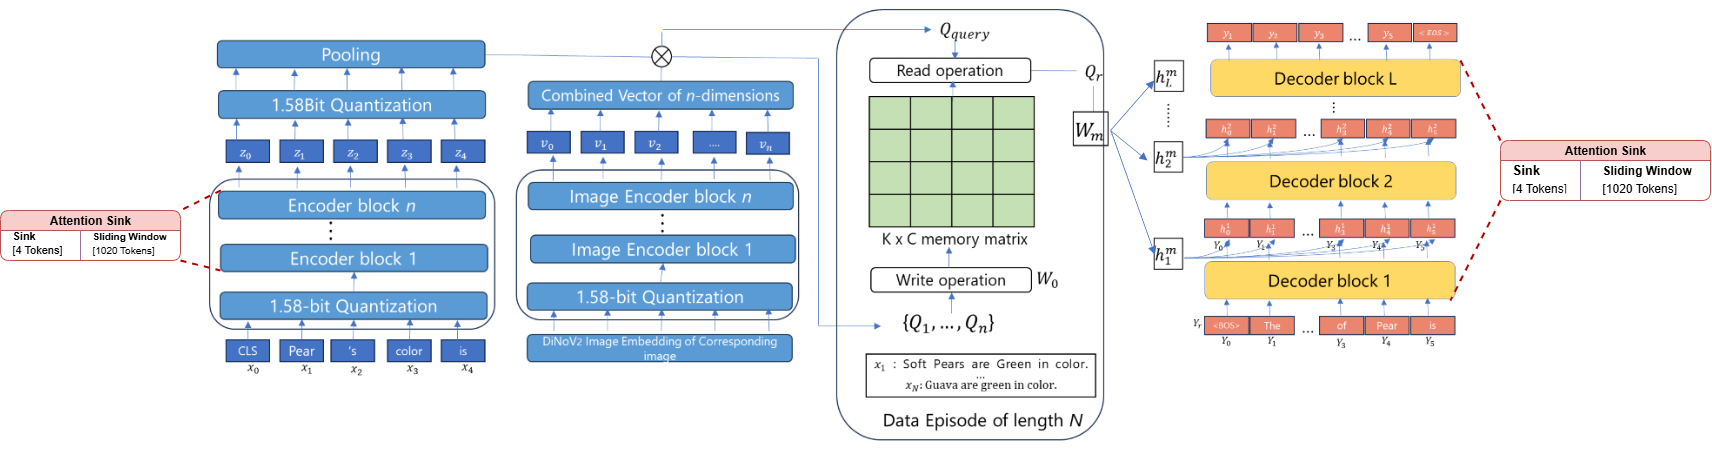
\includegraphics[width=\textheight]{../BabyLM_new/FIG/BitMar-Architecture.png}
    \caption{\textbf{BitMar Architecture.} The model processes multimodal inputs: text tokens and DiNOv2-compressed image features. Quantized encoders (1.58-bit) generate compact text and vision embeddings ($z$, $v$), which are fused via cross-modal attention into shared query representations. A sliding-window attention mechanism enables long-context processing. A fixed episodic memory matrix ($K \times C$) stores and retrieves multimodal context vectors through quantized read/write weights, supporting optional SD-card offloading for edge deployment.}
    \label{fig:bitmar_arch}
\end{sidewaysfigure}

\section{Text Encoder}
\label{sec:bitmar_text_encoder}

\subsection{Architecture}
The BitMar text encoder is a lightweight quantized Transformer with 4 layers, hidden dimension $d{=}128$, and $h{=}4$ attention heads, supporting sequences of up to 256 tokens.

\subsection{Quantization}
Two levels of quantization are applied:

\paragraph{Weight Quantization.} All linear projection weights in MHSA and FFN sublayers are quantized to ternary values $\{-1, 0, +1\}$ using learned per-layer scaling factors $\gamma$:
\begin{equation}
    \hat{W} = \mathrm{RoundClip}\!\left(\frac{W}{\gamma + \epsilon},\ -1,\ 1\right), \quad \gamma = \frac{1}{nm}\sum_{i,j}|W_{ij}|
\end{equation}
where $\mathrm{RoundClip}(\cdot, a, b) = \max(a, \min(b, \mathrm{round}(\cdot)))$ maps each weight to the nearest ternary value. The scale $\gamma$ is the mean absolute value of the unquantized weight matrix, trained jointly with the network parameters.

\paragraph{Activation Quantization.} Token-wise activations are quantized to 8 bits using per-token max-abs scaling:
\begin{equation}
    \hat{\mathbf{x}}_t = \mathrm{round}\!\left(\frac{\mathbf{x}_t}{\max_j |x_{t,j}|} \times 127\right)
\end{equation}
This localized scaling preserves fine-grained detail for each token by adapting to that token's specific activation range.

\subsection{Attention Sinks for Long-Context Processing}
Attention sinks are injected into every self-attention layer to enable efficient long-sequence processing. With $S{=}4$ persistent sink tokens and a sliding window of $W{=}1{,}020$, the KV cache maintains global context anchors alongside recent tokens. When a new token arrives, the oldest window token is evicted, sink and window sets are merged, and positional indices are clamped to $[0,\ S + W - 1]$, yielding $O(S+W)$ memory regardless of sequence length.

\section{Vision Encoder}
\label{sec:bitmar_vision_encoder}

The vision branch leverages pretrained DiNOv2~\cite{oquab2024dinov2} to extract 768-dimensional patch features \emph{offline}, avoiding heavy backbone inference at deployment time. $2{\times}2$ average pooling reduces the patch count by $4\times$. A learned two-layer MLP bottleneck then compresses 768 $\rightarrow$ 128 dimensions:
\begin{align}
    \mathbf{z}^{(1)}_{\text{vis}} &= \mathrm{ReLU}(\mathbf{W}_1 \mathbf{x}_{\text{vis}} + \mathbf{b}_1), \\
    \mathbf{z}^{(2)}_{\text{vis}} &= \mathbf{W}_2 \mathbf{z}^{(1)}_{\text{vis}} + \mathbf{b}_2
\end{align}
where $\mathbf{W}_1 \in \mathbb{R}^{384 \times 768}$, $\mathbf{W}_2 \in \mathbb{R}^{128 \times 384}$. All subsequent fusion, memory, and decoder pathways operate in the 128-dimensional space.

\section{Cross-Modal Fusion}
\label{sec:bitmar_fusion}

Given pooled text tokens $\mathbf{Z} \in \mathbb{R}^{n_t \times 128}$ and compressed vision tokens $\mathbf{V}_{\text{img}} \in \mathbb{R}^{n_v \times 128}$, the fusion module applies standard cross-attention~\cite{vaswani2017attention} with text queries and vision keys/values:
\begin{equation}
    \mathrm{Attention}(\mathbf{Q}, \mathbf{K}, \mathbf{V}) = \mathrm{softmax}\!\left(\frac{\mathbf{Q}\mathbf{K}^\top}{\sqrt{d_k}}\right)\mathbf{V}
\end{equation}
All projection matrices use 1.58-bit ternary weights; softmax and residual/LN run in FP32. The fused output $\mathbf{F} \in \mathbb{R}^{n_t \times 128}$ is mean-pooled to a single query vector $\mathbf{q}_{\text{mem}} \in \mathbb{R}^{128}$ for memory retrieval.

An InfoNCE contrastive loss~\cite{oord2018representation} enforces cross-modal alignment:
\begin{equation}
    \mathcal{L}_{\text{cm}} = -\frac{1}{N}\sum_{i=1}^{N} \log \frac{\exp(\mathrm{sim}(\mathbf{z}_t^i, \mathbf{z}_v^i)/\tau)}{\sum_{j=1}^{N} \exp(\mathrm{sim}(\mathbf{z}_t^i, \mathbf{z}_v^j)/\tau)}
\end{equation}

\section{Episodic Memory Module}
\label{sec:bitmar_memory}

\subsection{Memory Matrix Specification}
The memory is a learnable matrix $\mathbf{M} \in \mathbb{R}^{K \times C}$ with $K{=}512$ slots and $C{=}128$ dimensions. Each slot stores a 128-dimensional latent vector summarizing multimodal context from past inputs.

\subsection{Writing Mechanism}
At step $t$, query $\mathbf{q}_t \in \mathbb{R}^{C}$ is written to the memory via learned write weights $\mathbf{W}_w \in \mathbb{R}^{K}$ using a soft outer-product update:
\begin{equation}
    \mathbf{M} \leftarrow \mathbf{M} + \alpha \cdot \mathbf{W}_w \, \mathbf{q}_t^\top
    \label{eq:bitmar_mem_write}
\end{equation}
where $\alpha{=}0.2$. This distributes the write proportionally across all slots, ensuring stability.

\subsection{Reading Mechanism}
Content-based addressing~\cite{graves2016dnc} produces the retrieved vector:
\begin{align}
    \mathbf{W}_r &= \mathrm{softmax}(\mathbf{M} \, \mathbf{q}_t) \in \mathbb{R}^K, \\
    \mathbf{M}_r &= \mathbf{W}_r^\top \mathbf{M} \in \mathbb{R}^{1 \times C}
    \label{eq:bitmar_mem_read}
\end{align}

\subsection{Regularization and Forgetting}
A Frobenius-norm penalty on successive updates prevents thrashing:
\begin{equation}
    \mathcal{L}_{\text{mem}} = \lambda \|\Delta\mathbf{M}\|_F^2, \quad \Delta\mathbf{M} = \mathbf{M}^{(t)} - \mathbf{M}^{(t-1)}
    \label{eq:bitmar_mem_reg}
\end{equation}
Usage-based forgetting additionally attenuates stale slots.

\begin{algorithm}[htbp]
\small
\caption{BitMar episodic memory read/write procedure.}
\label{alg:bitmar_memory}
\begin{algorithmic}[1]
\Require Query $\mathbf{q}_t \in \mathbb{R}^C$, Memory $\mathbf{M} \in \mathbb{R}^{K \times C}$,
\Statex \hspace{\algorithmicindent} write weights $\mathbf{W}_w \in \mathbb{R}^K$, write rate $\alpha$, regularization weight $\lambda$
\Ensure Updated memory $\mathbf{M}$, retrieved context vector $\mathbf{M}_r$
\State \textbf{Write:} $\mathbf{M} \leftarrow \mathbf{M} + \alpha \cdot \mathbf{W}_w \, \mathbf{q}_t^\top$
\State \textbf{Read weights:} $\mathbf{W}_r \leftarrow \mathrm{softmax}(\mathbf{M} \, \mathbf{q}_t)$
\State \textbf{Retrieve:} $\mathbf{M}_r \leftarrow \mathbf{W}_r^\top \mathbf{M}$
\State \textbf{Regularize:} $\mathcal{L}_{\text{mem}} \mathrel{+}= \lambda\|\mathbf{M}^{(t)} - \mathbf{M}^{(t-1)}\|_F^2$
\State \Return $\mathbf{M}$, $\mathbf{M}_r$
\end{algorithmic}
\end{algorithm}

\section{Decoder with Attention Sinks}
\label{sec:bitmar_decoder}

The decoder is a 4-layer causal Transformer ($d{=}128$, $h{=}4$, max 256 tokens) with the same attention sink mechanism as the encoder. At each step, the retrieved memory vector $\mathbf{M}_r$ is projected and injected as per-layer conditioning. The output projection (128 $\rightarrow$ 50{,}257 GPT-2 vocabulary) uses ternary weights; logit computation runs in FP32.

\section{Training Objectives and Adaptive Curriculum}
\label{sec:bitmar_training}

\subsection{Multi-Component Objective}
The total training objective combines three terms:
\begin{equation}
    \mathcal{L} = \mathcal{L}_{\text{lm}} + 1.5 \cdot \mathcal{L}_{\text{cm}} + 0.1 \cdot \mathcal{L}_{\text{mem}}
    \label{eq:bitmar_total}
\end{equation}
where $\mathcal{L}_{\text{lm}}$ is the standard language modeling cross-entropy, $\mathcal{L}_{\text{cm}}$ is the InfoNCE cross-modal alignment loss (weighted 1.5 to prioritize alignment), and $\mathcal{L}_{\text{mem}}$ is the memory consistency regularizer (weighted 0.1 as a light stabilizer).

\subsection{Adaptive Training Controller}
The Adaptive Training Controller (ATC) monitors a 200-step EMA of cross-modal cosine similarity. When the EMA drops $>0.12$ from its recent maximum (with $\geq$800-step cooldown), it randomly freezes one encoder or upweights $\mathcal{L}_{\text{cm}}$ for 1{,}500 steps, preventing modality collapse. Algorithm~\ref{alg:atc} formalizes this procedure.

\begin{algorithm}[htbp]
\small
\caption{Adaptive Training Controller (ATC) for modality collapse prevention.}
\label{alg:atc}
\begin{algorithmic}[1]
\Require EMA window $W_{\text{ema}}{=}200$, drop threshold $\delta{=}0.12$,
\Statex \hspace{\algorithmicindent} freeze duration $T_f{=}1{,}500$, cooldown $T_c{=}800$
\Require Cross-modal cosine similarity at step $t$:
\Statex \hspace{\algorithmicindent} $s_t = \cos(\mathbf{z}_t^{\text{text}},\, \mathbf{z}_t^{\text{vis}})$
\State $\bar{s}_0 \leftarrow s_0$;\enspace $s^*_0 \leftarrow s_0$;\enspace $\text{last\_intervention} \leftarrow -T_c$
\For{each training step $t$}
    \State $\bar{s}_t \leftarrow (1 - 1/W_{\text{ema}})\,\bar{s}_{t-1} + (1/W_{\text{ema}})\,s_t$ \Comment{update EMA}
    \State $s^*_t \leftarrow \max(s^*_{t-1},\, \bar{s}_t)$ \Comment{track peak EMA}
    \If{$\bar{s}_t < s^*_t - \delta$ \textbf{and} $t - \text{last\_intervention} \geq T_c$}
        \State Sample $a \sim \mathrm{Uniform}\{\texttt{freeze\_text},\; \texttt{freeze\_vision},\; \texttt{boost\_cm}\}$
        \If{$a = \texttt{freeze\_text}$}
            \State Freeze text encoder parameters for $T_f$ steps
        \ElsIf{$a = \texttt{freeze\_vision}$}
            \State Freeze vision MLP parameters for $T_f$ steps
        \Else
            \State Set $w_{\text{cm}} \leftarrow 3.0$ for $T_f$ steps, then restore to 1.5
        \EndIf
        \State $\text{last\_intervention} \leftarrow t$
    \EndIf
    \State Update via AdamW: $\mathcal{L} = \mathcal{L}_{\text{lm}} + w_{\text{cm}}\,\mathcal{L}_{\text{cm}} + 0.1\,\mathcal{L}_{\text{mem}}$
\EndFor
\end{algorithmic}
\end{algorithm}

\section{Dataset and Training Configuration}
\label{sec:bitmar_dataset}

Training uses a 100M-token corpus: 50M multimodal tokens from CC3M~\cite{sharma2018cc3m} and Localized Narratives~\cite{ponttuset2020localizednarratives} (with precomputed DiNOv2 features), and 50M text-only tokens from the BabyLM 2025 corpus~\cite{charpentier2025babylm} spanning BNC, CHILDES, Gutenberg, OpenSubtitles, Simple English Wikipedia, and Switchboard. A 1M-token hold-out tracks alignment and perplexity throughout training. Training configuration is summarized in Table~\ref{tab:bitmar_training_config}.

\begin{table}[htbp]
\centering
\caption{\textbf{BitMar training configuration.} Key hyperparameters used during the 10-epoch training run on the 100M-token corpus.}
\label{tab:bitmar_training_config}
\begin{tabular}{ll}
\toprule
\textbf{Hyperparameter} & \textbf{Value} \\
\midrule
Text encoder layers & 4 \\
Hidden dimension $d$ & 128 \\
Memory slots $K$ & 512 \\
Memory dimension $C$ & 128 \\
Sink tokens $S$ & 4 \\
Sliding window $W$ & 1{,}020 \\
Cross-modal loss weight & 1.5 \\
Memory consistency weight & 0.1 \\
ATC drop threshold & 0.12 \\
ATC freeze duration (steps) & 1{,}500 \\
ATC minimum interval (steps) & 800 \\
Optimizer & AdamW8bit \\
Learning rate & $2 \times 10^{-4}$ \\
Effective batch size & 128 \\
Precision & FP16 \\
Training hardware & NVIDIA A6000 \\
\bottomrule
\end{tabular}
\end{table}

\section{Quantization Effectiveness Analysis}
\label{sec:bitmar_quant_analysis}

The quantization effectiveness metric $E_q$ measures the fraction of ternary weights set to zero across all quantized layers. A higher $E_q$ indicates greater effective compression. As shown in Figure~\ref{fig:bitmar_quant}, $E_q$ stabilizes at 42.8\% by the end of training, demonstrating that BitMar learns dense representations within its compressed ternary space. Early growth (0--200k steps) is step-like as encoders adapt; after 400k steps, growth smooths toward convergence.

\begin{figure}[!htb]
    \centering
    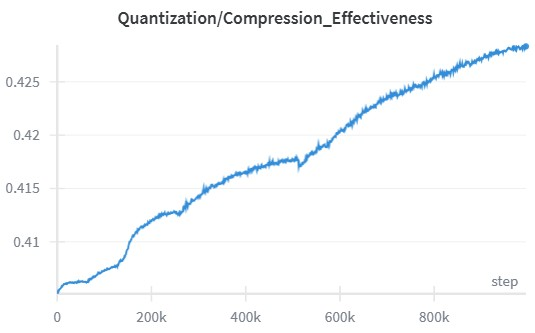
\includegraphics[width=0.75\linewidth]{../BabyLM_new/FIG/quantization.jpg}
    \caption{\textbf{Quantization effectiveness over training.} $E_q$ (fraction of ternary weights set to zero) stabilizes at 42.8\%, demonstrating efficient compression without downstream performance degradation.}
    \label{fig:bitmar_quant}
\end{figure}

\begin{figure}[!htb]
    \centering
    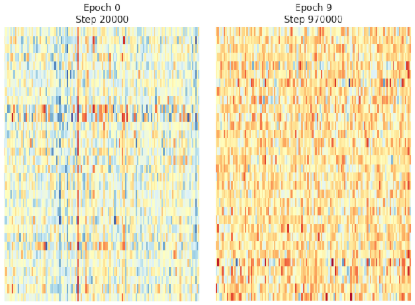
\includegraphics[width=\textwidth]{../BabyLM_new/FIG/BitMar-HeatMapComparisons.png}
    \caption{\textbf{Episodic memory slot activation patterns across training checkpoints.} Each row corresponds to a different checkpoint, ranging from early training (top, Epoch 0, step 20k) to late training (bottom, Epoch 9, step 97k). Early checkpoints show scattered, weak activations with minimal slot specialization. By the final checkpoint, memory slots develop strongly differentiated activation profiles, with specific slots specializing for distinct semantic categories. This convergence confirms that the episodic memory organizes stored representations by semantic content rather than recency.}
    \label{fig:bitmar_heatmap}
\end{figure}

\section{Experimental Results}
\label{sec:bitmar_results}

\subsection{Language Understanding Benchmarks}

\begin{table}[htbp]
\centering
\caption{\textbf{Language understanding benchmark performance.} \checkmark = natively 1-bit trained. Scores are accuracy (\%). WG = WinoGrande, CQA = CommonsenseQA, ARC-E = ARC-Easy.}
\label{tab:bitmar_lm_benchmarks}
\resizebox{\textwidth}{!}{%
\begin{tabular}{lcccccccc}
\toprule
\textbf{Model} & \textbf{Params} & \textbf{1-bit} & \textbf{ARC-E} & \textbf{BoolQ} & \textbf{HSwag} & \textbf{WG} & \textbf{CQA} & \textbf{MMLU} \\
\midrule
Bonsai 0.5B        & 500M & \checkmark & 58.25 & 58.44 & 48.01 & 54.46 & 18.43 & 25.74 \\
OLMo-BitNet 1B     & 1B   & \checkmark & 25.38 & 52.48 & 25.88 & 51.54 & 19.49 & 25.47 \\
Falcon3-1.58bit 7B & 7B   & $\times$   & 65.03 & 72.14 & 59.46 & 60.14 & 67.08 & 42.79 \\
LLaMA3-8B-1.58     & 8B   & $\times$   & 70.71 & 68.38 & 68.56 & 60.93 & 28.50 & 35.04 \\
BitNet b1.58 2B    & 2B   & \checkmark & 74.79 & 80.18 & 68.44 & 71.90 & 71.58 & 53.17 \\
\midrule
\textbf{BitMar-14M (Ours)} & 14M & \checkmark & 28.32 & \textbf{42.83} & 30.04 & \textbf{54.57} & 24.57 & 27.90 \\
\bottomrule
\end{tabular}%
}
\end{table}

Table~\ref{tab:bitmar_lm_benchmarks} compares BitMar-14M against low-bit quantized baselines. Despite being 35$\times$ smaller than the next-smallest baseline (Bonsai 0.5B), BitMar achieves competitive BoolQ (42.83\%) and WinoGrande (54.57\%), demonstrating strength in binary reasoning and coreference. ARC-Easy (28.32\%) and HellaSwag (30.04\%) trail larger models, reflecting capacity limits on multi-step commonsense reasoning.

\subsection{BabyLM Evaluation Suite}

\begin{table}[htbp]
\centering
\caption{\textbf{BitMar BabyLM evaluation.} Average finetuned NLP accuracy: 60.5\%.}
\label{tab:bitmar_babylm}
\begin{tabular}{llll}
\toprule
\textbf{Category} & \textbf{Task} & \textbf{Metric} & \textbf{Score} \\
\midrule
\multirow{7}{*}{Finetune NLP} & BoolQ & Accuracy & 66.5\% \\
 & MNLI & Accuracy & 42.3\% \\
 & MRPC & Accuracy & 69.1\% \\
 & MultiRC & Accuracy & 57.6\% \\
 & QQP & Accuracy & 70.2\% \\
 & RTE & Accuracy & 54.0\% \\
 & WSC & Accuracy & 63.5\% \\
\midrule
\multirow{3}{*}{Multimodal} & DevBench & Visual Vocab Acc. & 21.2\% \\
 & VQA & Accuracy & 21.4\% \\
 & Winoground & Accuracy & 23.8\% \\
\midrule
World Knowledge & EWoK & Accuracy & 24.9\% \\
\midrule
\multirow{3}{*}{Linguistic} & BLiMP & Accuracy & 48.7\% \\
 & Compositional & Accuracy & 51.5\% \\
 & Entity Tracking & Accuracy & 31.2\% \\
\midrule
Psycholinguistic & Reading Comp. & Score & 0.44 \\
\midrule
\multirow{2}{*}{Morphology} & Wug Adj. & Correlation & $-$0.16 \\
 & Wug Past & Correlation & $-$0.22 \\
\bottomrule
\end{tabular}
\end{table}

BitMar achieves 60.5\% average across finetuned NLP benchmarks, with strengths in paraphrase detection (QQP: 70.2\%, MRPC: 69.1\%) and reading comprehension (BoolQ: 66.5\%). Multimodal tasks score 21--25\%, with the highest result on EWoK (24.9\%), plausibly due to episodic memory providing relevant context. Negative Wug morphology correlations ($-$0.16, $-$0.22) indicate systematic limits in morphological productivity under extreme compression.

\subsection{Episodic Memory Ablation}

\begin{table}[htbp]
\centering
\caption{\textbf{Inference efficiency with and without episodic memory.}}
\label{tab:bitmar_eff_ablation}
\begin{tabular}{lcc}
\toprule
\textbf{Metric} & \textbf{Memory On} & \textbf{Memory Off} \\
\midrule
Throughput (tok/s) & \textbf{57.3} & 7.7 \\
Latency/token (ms) & \textbf{17.3} & 129.8 \\
Energy (J) & \textbf{1.90} & 9.17 \\
RAM (MB) & \textbf{956} & 1{,}076 \\
\bottomrule
\end{tabular}
\end{table}

\begin{table}[htbp]
\centering
\caption{\textbf{Zero-shot accuracy deltas ($\Delta$ pp) with episodic memory enabled.}}
\label{tab:bitmar_acc_ablation}
\begin{tabular}{lc}
\toprule
\textbf{Task} & \textbf{$\Delta$ (pp)} \\
\midrule
Entity Tracking (Split 1) & +2.9 \\
Entity Tracking (Split 2) & +4.1 \\
COMPS & +3.4 \\
BLiMP & +0.6 \\
VQA & +3.4 \\
EWoK (Split 1) & $-$1.6 \\
EWoK (Split 2) & +1.0 \\
Winoground & $-$1.6 \\
DevBench & No effect \\
\bottomrule
\end{tabular}
\end{table}

Episodic memory provides 7.5$\times$ throughput improvement, 79\% energy reduction, and 11\% lower RAM usage. Zero-shot accuracy gains of 3--4 pp are consistent across entity tracking and visual question answering. Two regressions (Winoground $-$1.6pp, EWoK Split 1 $-$1.6pp) are attributed to the fixed-capacity memory occasionally introducing irrelevant context, a tradeoff inherent in any fixed-size retrieval system.

\section{Implementation Details}
\label{sec:bitmar_impl}

\subsection{Hyperparameters}

Table~\ref{tab:bitmar_arch_hyperparams} lists the architectural hyperparameters and Table~\ref{tab:bitmar_train_hyperparams} lists the training configuration.

\begin{longtable}{lp{6cm}}
\caption{\textbf{BitMar architectural hyperparameters.} Full specification of the 14M-parameter ternary-quantized architecture.}
\label{tab:bitmar_arch_hyperparams} \\
\toprule
\textbf{Hyperparameter} & \textbf{Value} \\
\midrule
\endfirsthead
\multicolumn{2}{c}{\tablename\ \thetable{} (continued)} \\
\toprule
\textbf{Hyperparameter} & \textbf{Value} \\
\midrule
\endhead
\midrule
\multicolumn{2}{r}{\textit{Continued on next page}} \\
\endfoot
\bottomrule
\endlastfoot
\multicolumn{2}{l}{\textit{Text Encoder}} \\
\quad Transformer layers & 4 \\
\quad Hidden dimension $d$ & 128 \\
\quad Attention heads $h$ & 4 \\
\quad Max sequence length & 256 tokens \\
\quad Weight quantization & Ternary $\{-1,0,+1\}$, learned per-layer scale \\
\quad Activation quantization & Per-token 8-bit max-abs, range $[-127,127]$ \\
\quad Attention sinks $S$ & 4 \\
\quad Sliding window $W$ & 1{,}020 \\
\midrule
\multicolumn{2}{l}{\textit{Vision Encoder}} \\
\quad Vision backbone & DiNOv2 (frozen, offline feature extraction) \\
\quad DiNOv2 feature dimension & 768 \\
\quad Spatial pooling & $2\times2$ average pooling \\
\quad MLP compression $\mathbf{W}_1$ & $\mathbb{R}^{384\times768}$ \\
\quad MLP compression $\mathbf{W}_2$ & $\mathbb{R}^{128\times384}$ \\
\quad Output dimension & 128 \\
\midrule
\multicolumn{2}{l}{\textit{Cross-Modal Fusion}} \\
\quad Fusion type & Cross-attention (text queries, vision K/V) \\
\quad Projection quantization & 1.58-bit ternary \\
\quad Fusion output & $\mathbf{F} \in \mathbb{R}^{n_t \times 128}$ \\
\quad Memory query pooling & Mean pooling $\rightarrow \mathbf{q}_{\text{mem}} \in \mathbb{R}^{128}$ \\
\midrule
\multicolumn{2}{l}{\textit{Episodic Memory}} \\
\quad Memory slots $K$ & 512 \\
\quad Memory dimension $C$ & 128 \\
\quad Write rate $\alpha$ & 0.2 \\
\quad Memory regularization $\lambda$ & 0.1 \\
\quad Addressing mechanism & Content-based (softmax inner product) \\
\midrule
\multicolumn{2}{l}{\textit{Decoder}} \\
\quad Transformer layers & 4 \\
\quad Hidden dimension & 128 \\
\quad Attention heads & 4 \\
\quad Max generation length & 256 tokens \\
\quad Attention sinks & Same as encoder \\
\quad Output vocabulary & GPT-2 BPE (50{,}257 tokens) \\
\quad Output projection & Ternary weights, FP32 logits \\
\end{longtable}

\begin{table}[htbp]
\centering
\caption{\textbf{BitMar training hyperparameters.} Optimizer, schedule, memory, and hardware settings used across the full 10-epoch run.}
\label{tab:bitmar_train_hyperparams}
\begin{tabular}{lp{5.5cm}}
\toprule
\textbf{Hyperparameter} & \textbf{Value} \\
\midrule
\multicolumn{2}{l}{\textit{Training}} \\
\quad Optimizer & AdamW8bit \\
\quad Learning rate & $2 \times 10^{-4}$ \\
\quad Cosine restart $T_0$ & 1{,}000 steps \\
\quad Cosine restart $T_{\text{mult}}$ & 2 \\
\quad Min learning rate $\eta_{\min}$ & $0.1 \times \text{lr}$ \\
\quad Effective batch size & 128 \\
\quad Training epochs & 10 \\
\quad Precision & FP16 \\
\quad Gradient checkpointing & Yes \\
\quad Training hardware & NVIDIA A6000 \\
\midrule
\multicolumn{2}{l}{\textit{Loss Weights}} \\
\quad Language modeling $\mathcal{L}_{\text{lm}}$ & 1.0 \\
\quad Cross-modal contrastive $\mathcal{L}_{\text{cm}}$ & 1.5 \\
\quad Memory consistency $\mathcal{L}_{\text{mem}}$ & 0.1 \\
\midrule
\multicolumn{2}{l}{\textit{Adaptive Training Controller}} \\
\quad EMA window & 200 steps \\
\quad Drop threshold & 0.12 \\
\quad Freeze/boost duration & 1{,}500 steps \\
\quad Min intervention interval & 800 steps \\
\bottomrule
\end{tabular}
\end{table}

\subsection{Training Corpus}

Table~\ref{tab:bitmar_dataset_stats} details the composition of BitMar's 101M-token training corpus. Multimodal pairs (50M tokens) from CC3M and Localized Narratives provide visual-language grounding; text-only data (50M tokens) from six sources provides linguistic coverage. A 1M-token stratified hold-out set is reserved for evaluation.

\begin{table}[htbp]
\centering
\caption{\textbf{BitMar training corpus composition.} The 101M-token corpus combines 50M multimodal tokens and 50M text-only tokens, with a 1M-token stratified hold-out set.}
\label{tab:bitmar_dataset_stats}
\begin{tabular}{llr}
\toprule
\textbf{Type} & \textbf{Source} & \textbf{Tokens} \\
\midrule
\multirow{2}{*}{Multimodal (50M)} & CC3M (Conceptual Captions) & $\sim$28M \\
 & Localized Narratives & $\sim$22M \\
\midrule
\multirow{6}{*}{Text-only (50M)} & BNC Spoken & $\sim$10M \\
 & CHILDES & $\sim$5M \\
 & Gutenberg & $\sim$12M \\
 & OpenSubtitles & $\sim$10M \\
 & Simple English Wikipedia & $\sim$5M \\
 & Switchboard & $\sim$8M \\
\midrule
Hold-out & Mixed (stratified) & 1M \\
\midrule
\textbf{Total} & & \textbf{101M} \\
\bottomrule
\end{tabular}
\end{table}

\subsection{Tokenizer and Preprocessing}

BitMar uses the GPT-2 Byte Pair Encoding (BPE) tokenizer with a vocabulary size of 50{,}257 tokens. Text sequences exceeding 256 tokens are truncated; shorter sequences are padded. DiNOv2 visual features are extracted offline using a frozen DiNOv2 (large) backbone, storing $2\times2$-pooled 768-dimensional patch features as memory-mapped \texttt{.npy} files. During training, features are loaded with on-the-fly compression to reduce I/O overhead. Each multimodal sample is an (image, caption) pair, with the caption tokenized using the GPT-2 BPE tokenizer.

\subsection{External Memory Offloading}

For memory-constrained devices, the memory matrix $\mathbf{M}$ can be offloaded to external storage via a utility that saves and loads memory tensors without gradient tracking. This preserves the persistent memory state between sessions without increasing runtime RAM usage. The offload is triggered automatically when device RAM drops below a configurable threshold, making BitMar deployable on hardware with as little as 512~MB RAM.

\section{Lessons Learned and Research Directions}
\label{sec:bitmar_lessons}

BitMar validates three design hypotheses that directly motivated EmberVLM:

\paragraph{Validated: episodic memory is compatible with and beneficial for quantized multimodal models.} The efficiency gains and accuracy improvements confirm that episodic memory can replace heavy long-range attention even under aggressive 1.58-bit quantization.

\paragraph{Validated: 1.58-bit quantization is compatible with cross-modal fusion.} BabyLM multimodal task performance demonstrates that ternary weights support meaningful cross-modal alignment at 14M parameters.

\paragraph{Open: Can episodic memory address hallucination?} BitMar's memory improves coherence but has no mechanism for detecting visually ungrounded tokens. This gap directly motivated the Visual Absence Refiner in EmberVLM (Section~\ref{sec:embervlm_refiner}).

\paragraph{Open: Can the architecture scale to mission-critical classification?} BitMar's evaluation is primarily generative. Whether memory-augmented tiny VLMs can achieve reliable multi-label classification in safety-critical settings required a dedicated training pipeline and evaluation framework: the EmberVLM design.

\paragraph{Open: Can memory be truly adaptive at deployment?} BitMar's memory is essentially static at deployment: slots do not update after training. EmberVLM's novelty-triggered online writes (Section~\ref{sec:memory_novelty}) directly address this gap.

        \chapter{EmberVLM: Efficient Edge Vision-Language Model}
\label{cha:embervlm}

This chapter presents EmberVLM, the primary architectural contribution of this thesis. EmberVLM is a 164M total parameter (40M trainable) tiny VLM purpose-built for reliable mission-critical inference under strict edge-deployment constraints. It builds directly on the design principles established in BitMar (Chapter~\ref{cha:bitmar}), scaling to a more capable backbone while introducing two novel modules: the Episodic Memory Module and the Visual Absence (VA) Refiner.

\section{Overview and Design Philosophy}
\label{sec:embervlm_overview}

Figure~\ref{fig:embervlm_arch} illustrates the complete EmberVLM architecture. EmberVLM is guided by three design principles:

\begin{enumerate}
    \item \textbf{Compositional efficiency}: separate frozen pretrained representations (DINOv2-Small for visual perception, SmolLM-135M for linguistic priors) from a compact trainable core (40M parameters). This preserves the general capabilities of large pretraining while keeping training cost and carbon emissions minimal.
    \item \textbf{Memory-augmented reliability}: treat episodic memory not as a static knowledge base but as a dynamically loadable, deployment-time cache that provides contextual biases drawn from prior field experience. Memory breaks the traditional latency--accuracy tradeoff by providing near-zero-cost retrieval from a compact on-device matrix.
    \item \textbf{Mechanistic hallucination control}: instead of suppressing hallucinations through additional supervision or retraining, identify and penalize visually ungrounded tokens at inference time by monitoring the model's own internal neuron-level activation patterns.
\end{enumerate}

\begin{sidewaysfigure}[p]
    \centering
    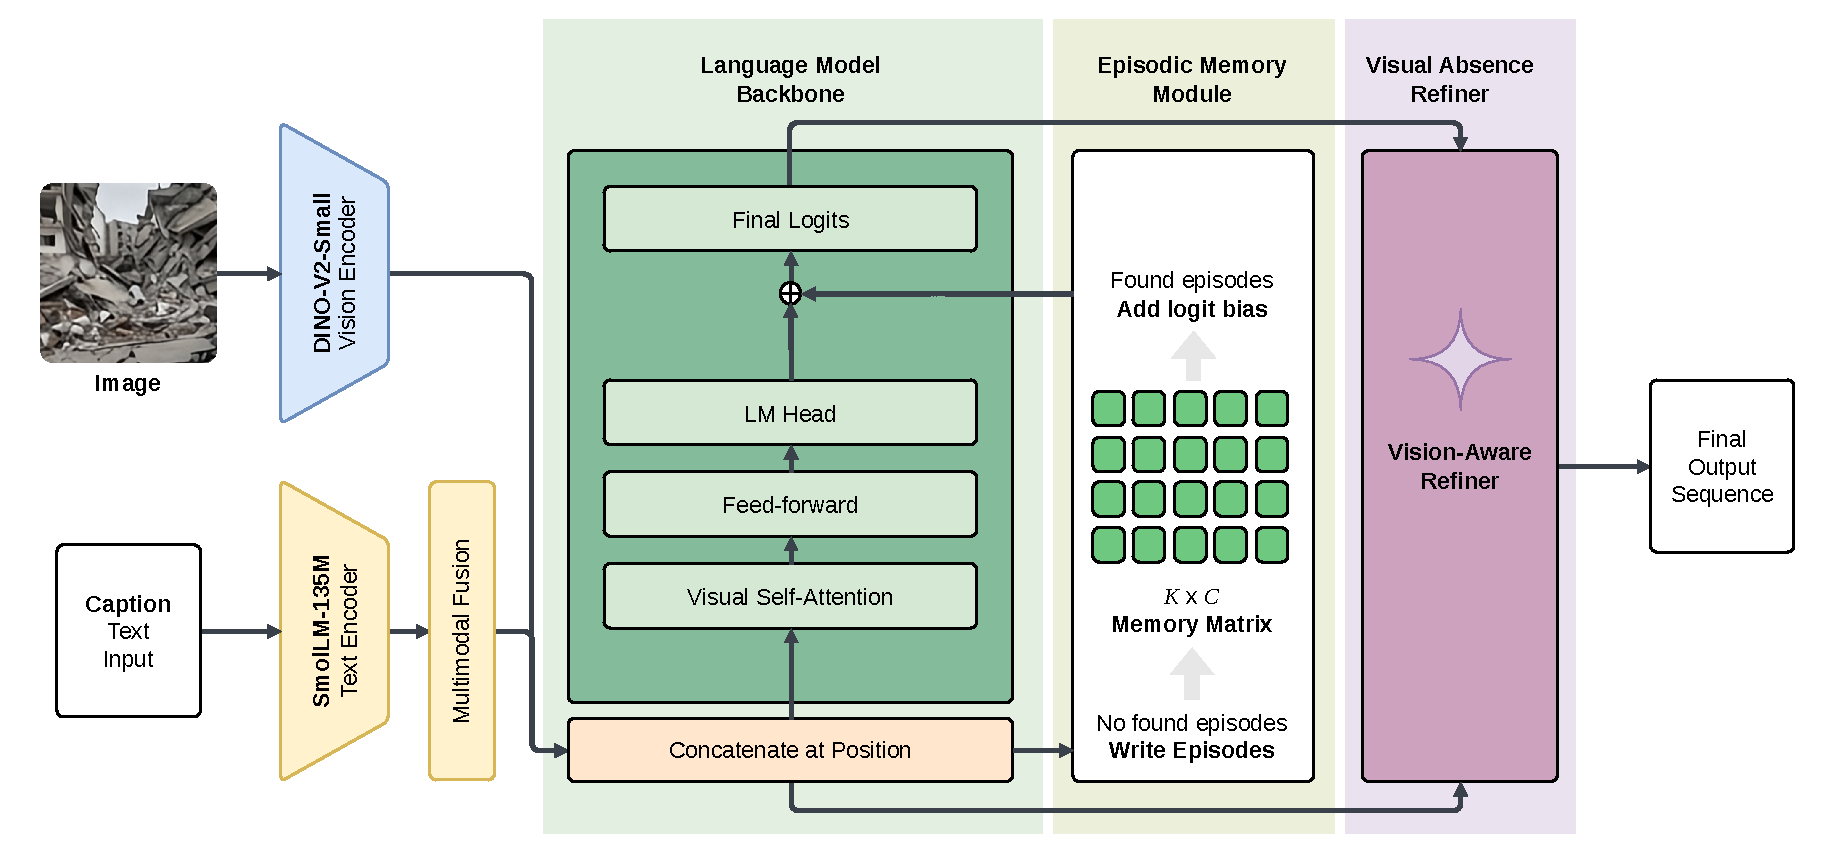
\includegraphics[width=\textheight]{../EmberVLM/paper-template-Latest/figures/main_diagram.pdf}
    \caption{\textbf{EmberVLM architecture overview.} The system integrates a frozen DINOv2-Small vision encoder, a SmolLM-135M language backbone, a Stable Gated Fusion module, an Episodic Memory Module, and the Visual Absence (VA) Refiner. Solid arrows denote forward-pass data flow; the memory matrix is outside the gradient graph and is updated algebraically at deployment time.}
    \label{fig:embervlm_arch}
\end{sidewaysfigure}

\section{Base Multimodal Pipeline}
\label{sec:embervlm_base}

\subsection{Vision Encoder}
EmberVLM employs DINOv2-Small~\cite{oquab2024dinov2} as the frozen visual perception module (21.1M parameters). The encoder aggressively compresses an input image $X_v$ into a minimal sequence of $N_v{=}8$ visual tokens with feature dimension $d_{\text{vis}}{=}384$. DINOv2-Small's self-supervised training provides robust visual features without task-specific supervision, and freezing it throughout training preserves general visual priors while contributing zero parameters to the trainable budget.

\subsection{Language Backbone}
SmolLM-135M~\cite{allal2024smollm} serves as both the text encoder and the language modeling backbone (135M parameters). SmolLM-135M is frozen in Stages 1, 3, and 4, and fully unfrozen end-to-end in Stage 2 (Multimodal Instruction Tuning). This staged approach allows the model to first learn cross-modal alignment while preserving linguistic priors, then adapt the full backbone to complex multimodal instruction following.

\subsection{Parameter Breakdown}

Figure~\ref{fig:embervlm_params_dist} illustrates the distribution of parameters across components. Of the 164M total parameters, only 40M (24.4\%) are updated during training; the remaining 75.6\% are frozen pretrained representations that contribute visual and linguistic priors at zero training cost.

\begin{figure}[!htb]
    \centering
    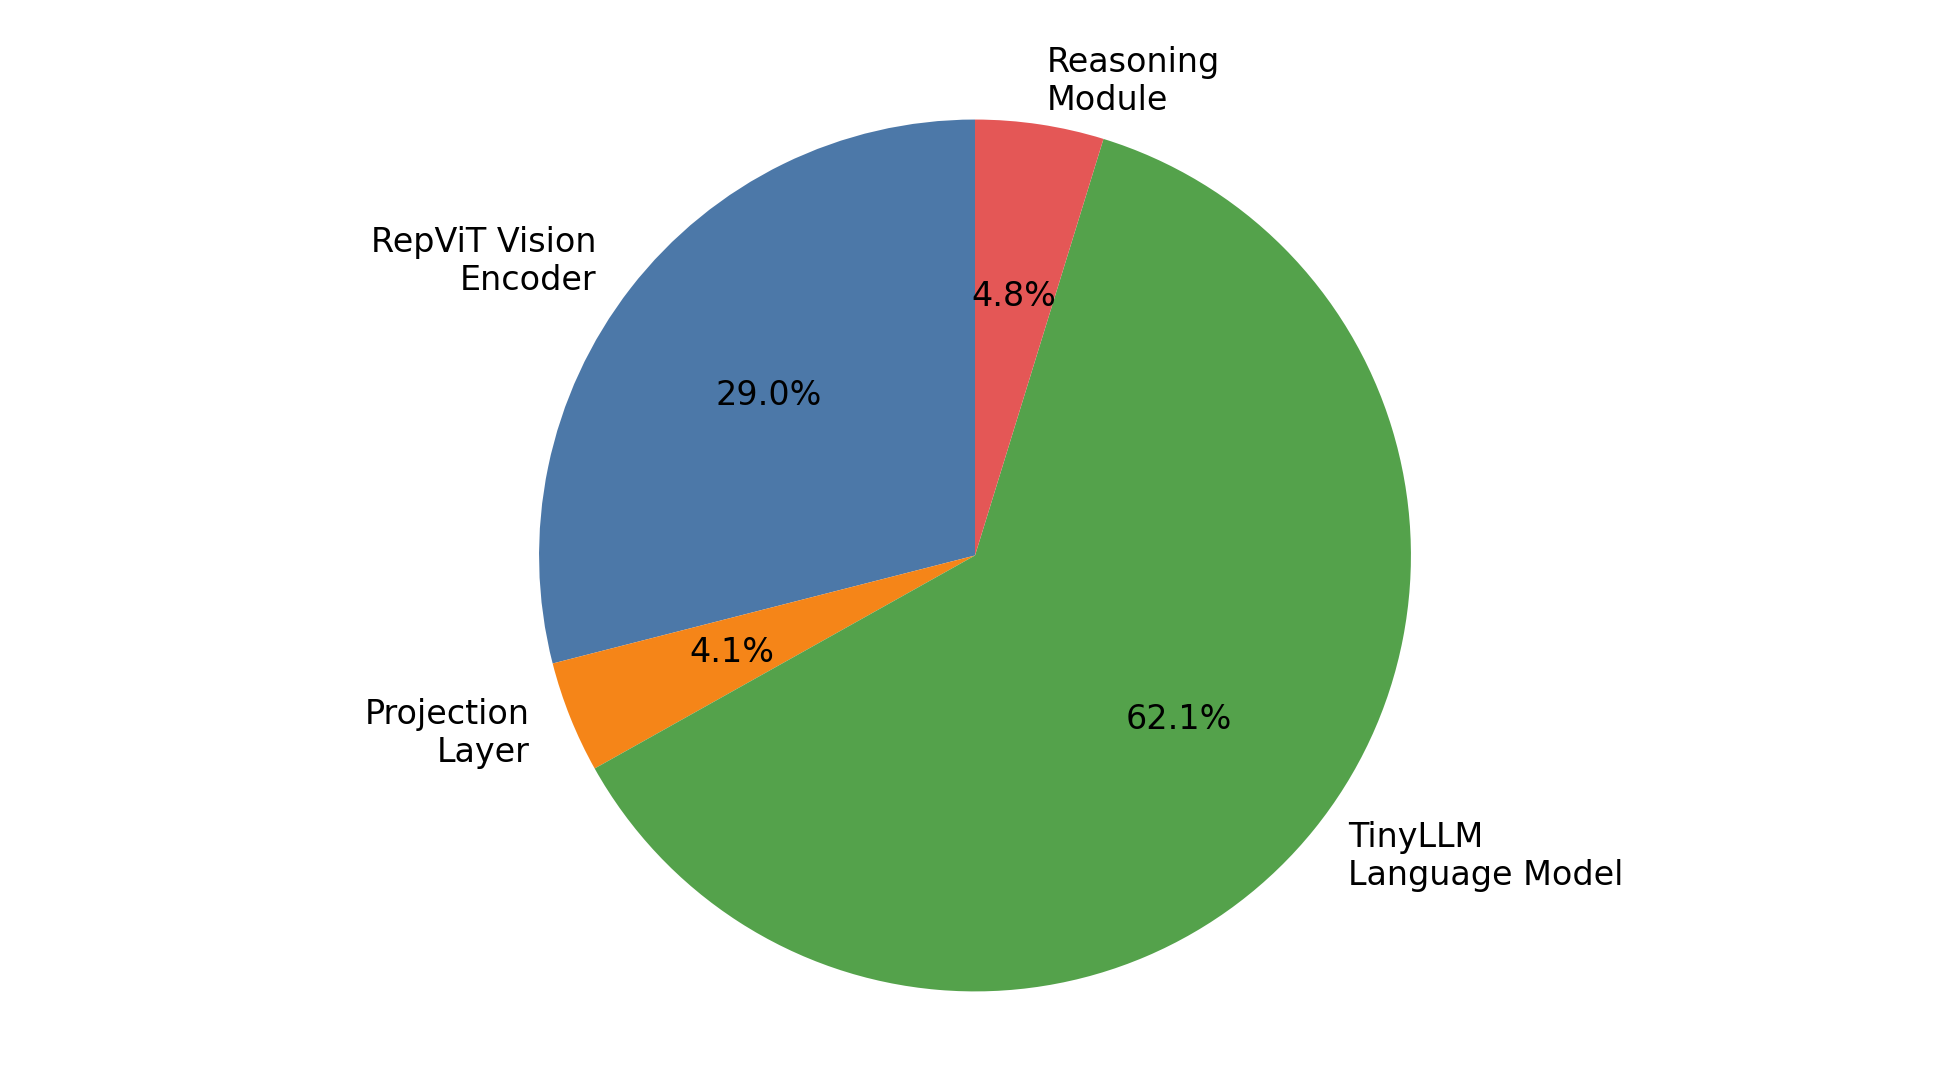
\includegraphics[width=0.65\linewidth]{../EmberVLM/paper-template-Latest/figures/embervlm_param_distribution.png}
    \caption{\textbf{EmberVLM parameter distribution.} DINOv2-Small (21.1M) and the frozen layers of SmolLM-135M account for the majority of total parameters and are never updated. The 40M trainable parameters are concentrated in the Fusion Module, bottleneck adapter, and Reasoning Head.}
    \label{fig:embervlm_params_dist}
\end{figure}

\begin{table}[htbp]
\centering
\caption{\textbf{EmberVLM parameter breakdown.} Total: 164M parameters, 40M trainable.}
\label{tab:embervlm_params}
\resizebox{\textwidth}{!}{%
\begin{tabular}{llcc}
\toprule
\textbf{Component} & \textbf{Params (M)} & \textbf{Trainable} & \textbf{Frozen Stages} \\
\midrule
DINOv2-Small (vision encoder) & 21.1 & --- & All stages \\
SmolLM-135M (text enc. + backbone) & 135.0 & Partial & 1, 3, 4 \\
Fusion Module (cross-attn + gate) & 7.27 & \checkmark & None \\
Bottleneck adapter & 0.06 & \checkmark & None \\
Reasoning \& Action Head & 0.57 & \checkmark & 1, 2 \\
\midrule
\textbf{Total} & \textbf{164.0} & \textbf{40M} & --- \\
\bottomrule
\end{tabular}%
}
\end{table}

\begin{table}[htbp]
\centering
\caption{\textbf{EmberVLM architectural specification.} Component-level summary of the 164M-parameter system, including encoder, backbone, memory, and VA Refiner configuration.}
\label{tab:embervlm_arch_spec}
\begin{tabular}{ll}
\toprule
\textbf{Component} & \textbf{Specification} \\
\midrule
Vision encoder & DINOv2-Small (21.1M, frozen) \\
Visual tokens $N_v$ & 8 \\
Visual feature dim $d_{\text{vis}}$ & 384 \\
Language backbone & SmolLM-135M (135M) \\
Language feature dim $d_{\text{lang}}$ & 576 \\
Bottleneck adapter dim & 48 \\
Vision gate initialization $\alpha$ & 2.5 \\
Episodic memory slots $K$ & 512 \\
Episodic memory dim $C$ & 576 \\
Memory size (fp32) & $\approx$1.2 MB \\
VA Refiner hook layers & 10--14 (SmolLM-135M FFN) \\
VA Refiner neuron count & 128 (top-$k$ per layer) \\
VA Refiner $\lambda$ & 0.5 \\
Visual threshold $p_{\text{VA}}$ & 0.6 \\
Non-visual threshold $p_{\text{VA}}$ & 0.8 \\
Latent CoT temperature $\tau$ & 0.07 \\
\bottomrule
\end{tabular}
\end{table}

\section{Stable Gated Fusion}
\label{sec:embervlm_fusion}

Raw visual tokens from DINOv2-Small (dimension 384) are projected into the language backbone's token embedding space ($d_{\text{lang}}{=}384$) via a parameter-efficient bottleneck adapter ($d_{\text{bottleneck}}{=}48$). A learnable vision gate scalar $\alpha$ (initialized to 2.5) dynamically scales the adapted visual influence:
\begin{equation}
    V_{\text{fused}} = \sigma(\alpha) \cdot \mathrm{LayerNorm}(V_{\text{adapt}})
    \label{eq:embervlm_gate}
\end{equation}
where $\sigma$ denotes the sigmoid activation. At initialization, $\sigma(2.5) \approx 0.92$, so visual influence starts near-full and becomes learnable rather than fixed. This gate allows the model to calibrate how much visual influence to apply during alignment learning, preventing early-stage visual features from overwhelming linguistic priors.

The gated visual tokens are interleaved with textual embeddings to form the joint context sequence processed by the language backbone.

\section{Task-Specific Adaptation: Top-$K$ Robot Selection Head}
\label{sec:embervlm_head}

While EmberVLM supports standard autoregressive generation, autoregressive decoding is inefficient and error-prone for mission-critical tactical deployment. For the primary robot selection task, the standard language modeling head is bypassed. Instead, final hidden states from the language backbone are mean-pooled to produce a dense incident representation $\mathbf{h}_{\text{pool}}$. A \textit{Reasoning and Action Head} MLP maps $\mathbf{h}_{\text{pool}}$ to a probability distribution over the robot fleet (Drone, Underwater Robot, Humanoid, Wheeled, Legged):
\begin{equation}
    \mathbf{p}_{\text{robot}} = \mathrm{softmax}\!\left(\mathrm{MLP}(\mathbf{h}_{\text{pool}})\right)
\end{equation}
This framing decouples general scene comprehension from tactical execution. Avoiding autoregressive decoding eliminates the token-by-token latency overhead, keeping total trainable parameters strictly under 40M.

\section{Episodic Memory Module}
\label{sec:embervlm_memory}

\subsection{Overview and Distinction from BitMar}
EmberVLM's episodic memory differs fundamentally from BitMar's gradient-trained memory. BitMar's memory matrix is updated via backpropagation and is static at deployment. EmberVLM's memory has three key properties:
\begin{itemize}
    \item \textbf{Outside the gradient graph}: the memory matrix is not differentiated through, as confirmed in the supplementary material.
    \item \textbf{Pre-populated offline}: populated from the training split during a READ\_ONLY pre-population phase before evaluation.
    \item \textbf{Updatable online at deployment}: in ONLINE\_UPDATE mode, new embeddings are written to memory during inference without weight updates, enabling adaptation to novel scenarios.
\end{itemize}

\subsection{Memory Matrix Specification}
The memory matrix $\mathbf{M} \in \mathbb{R}^{K \times C}$ has $K{=}512$ slots and $C{=}576$ feature dimensions, alongside an associated covariance matrix. Physical size: $512 \times 576 \times 4$ bytes $\approx$ 1.2~MB (fp32). The dimension $C{=}576$ matches the SmolLM-135M token embedding dimension, allowing direct residual injection of retrieved memory into the generation process without additional projection overhead.

\subsection{Scope Detector}
Before engaging memory retrieval, the incoming multimodal embedding $\mathbf{z}$ is evaluated by a lightweight Scope Detector: a 2-layer MLP binary classifier outputting $p(\text{in-scope})$. If $p < 0.5$, the query is deemed out-of-scope and the model defaults to parametric generation without memory. If $p \geq 0.5$, the fast memory retrieval path activates.

The scope detector serves as a gating mechanism that prevents irrelevant historical episodes from contaminating queries about novel or out-of-distribution scenes. Without scope detection, the memory module would apply retrieved context to every query, potentially degrading performance on genuinely novel scenarios.

\subsection{Memory Addressing and Retrieval}
When in-scope, normalized addressing weights $w_k$ over all $K$ memory slots are computed via Gaussian distance-based addressing:
\begin{equation}
    w_k = \frac{\exp\!\left(-\dfrac{\|\mathbf{z} - \mathbf{M}_k\|^2}{2\alpha\nu\tau}\right)}{\displaystyle\sum_{j=1}^{K} \exp\!\left(-\dfrac{\|\mathbf{z} - \mathbf{M}_j\|^2}{2\alpha\nu\tau}\right)}
    \label{eq:embervlm_mem_address}
\end{equation}
where $\alpha$, $\nu$, $\tau$ represent the update strength, variance, and temperature scaling factors, respectively. The retrieved memory readout $\mathbf{z}_m = \sum_k w_k \mathbf{M}_k$ is passed through the language model's unembedding head and added residually to the raw predictive logits, organically biasing generation toward historically successful resolutions.

This mechanism is more sophisticated than BitMar's content-based addressing in that it includes explicit variance ($\nu$) and temperature ($\tau$) parameters that control the sharpness of retrieval, allowing fine-tuned control over how broadly or narrowly the model draws from past experience.

\subsection{Novelty Detection and Dynamic Writes}
\label{sec:memory_novelty}
The novelty of an incoming embedding $\mathbf{z}$ is defined as:
\begin{equation}
    \sigma(\mathbf{z} \mid \mathbf{M}) = \min_k \|\mathbf{z} - \mathbf{M}_k\|^2
\end{equation}
If this minimum-distance novelty score exceeds a predefined threshold, the incident is classified as a fundamentally new experience. The system executes a single-shot recursive algebraic update using a linear solve over the residual difference between the new embedding and the current memory readout, updating both $\mathbf{M}$ and the covariance matrix.

When the memory reaches $K$-slot capacity, a hybrid Least Recently Used and Least Frequently Used (LRU-LFU) eviction policy selects the slot to overwrite. LRU alone risks discarding slots encoding critical rare morphologies (e.g., Underwater Robot, which appears in only 13 of the 103 validation samples); LFU alone risks retaining stale commonly-accessed but no-longer-relevant episodes. The hybrid policy balances recency and importance.

\subsection{Stage 5 Knowledge Consolidation}
During an optional Stage 5 consolidation phase, the frozen memory matrix acts as a teacher: an MSE alignment loss distills explicitly retrieved knowledge directly into the model's parametric weights. This ensures that frequently accessed experiences become ingrained in base model weights, freeing memory slots for new encounters. Stage 5 is not applied in any of the main paper evaluation results; it is a deployment-phase enhancement.

\subsection{Complete Memory Inference Procedure}

Algorithm~\ref{alg:embervlm_memory} summarizes the full episodic memory procedure executed at each inference step, unifying scope detection, Gaussian retrieval, novelty-triggered writes, and LRU-LFU eviction into a single coherent procedure.

\begin{algorithm}[htbp]
\small
\caption{EmberVLM episodic memory: scope detection, retrieval, novelty write, and LRU-LFU eviction.}
\label{alg:embervlm_memory}
\begin{algorithmic}[1]
\Require Query $\mathbf{z} \in \mathbb{R}^C$, memory $\mathbf{M} \in \mathbb{R}^{K \times C}$, covariance $\boldsymbol{\Sigma}$,
\Statex \hspace{\algorithmicindent} novelty threshold $\theta$, LRU-LFU balance $\gamma$,
\Statex \hspace{\algorithmicindent} mode $\in \{\texttt{OFF},\; \texttt{READ\_ONLY},\; \texttt{ONLINE\_UPDATE}\}$
\Ensure Residual logit bias $\Delta\mathbf{l}$, updated $\mathbf{M}$
\If{mode $= \texttt{OFF}$}
    \State \Return $\Delta\mathbf{l} \leftarrow \mathbf{0}$ \Comment{memory bypassed}
\EndIf
\State $p_{\text{scope}} \leftarrow \text{ScopeDetector}(\mathbf{z})$ \Comment{2-layer MLP binary classifier}
\If{$p_{\text{scope}} < 0.5$}
    \State \Return $\Delta\mathbf{l} \leftarrow \mathbf{0}$ \Comment{out-of-scope: use parametric generation}
\EndIf
\State $w_k \leftarrow \exp\!\bigl(-\|\mathbf{z} - \mathbf{M}_k\|^2 / (2\alpha\nu\tau)\bigr)$ for $k=1,\ldots,K$
\State $\mathbf{w} \leftarrow \mathbf{w} / \textstyle\sum_k w_k$ \Comment{Gaussian addressing weights}
\State $\mathbf{z}_m \leftarrow \textstyle\sum_k w_k \mathbf{M}_k$ \Comment{weighted memory readout}
\State $\Delta\mathbf{l} \leftarrow \text{UnembeddingHead}(\mathbf{z}_m)$ \Comment{residual logit bias}
\If{mode $= \texttt{ONLINE\_UPDATE}$}
    \State $\sigma_{\text{nov}} \leftarrow \min_k \|\mathbf{z} - \mathbf{M}_k\|^2$ \Comment{novelty score}
    \If{$\sigma_{\text{nov}} > \theta$} \Comment{novel: write to memory}
        \If{empty slot $k^*$ available}
            \State $k^* \leftarrow$ index of first empty slot
        \Else \Comment{LRU-LFU hybrid eviction}
            \State $k^* \leftarrow \arg\max_k\bigl[\gamma \cdot \text{age}(k) - (1{-}\gamma) \cdot \text{freq}(k)\bigr]$
        \EndIf
        \State $\mathbf{M}_{k^*} \leftarrow \mathbf{z}$; update $\boldsymbol{\Sigma}$; reset age/freq for $k^*$
    \EndIf
\EndIf
\State \Return $\Delta\mathbf{l}$, $\mathbf{M}$
\end{algorithmic}
\end{algorithm}

\subsection{Memory Operating Modes}

Three memory modes are available at deployment time, as specified in Table~\ref{tab:memory_modes_spec}.

\begin{table}[htbp]
\centering
\caption{\textbf{EmberVLM episodic memory operating modes.} The three runtime modes control whether the memory matrix is read, written, or inactive during inference.}
\label{tab:memory_modes_spec}
\begin{tabularx}{\textwidth}{lX}
\toprule
\textbf{Mode} & \textbf{Description} \\
\midrule
OFF & Memory matrix is zeroed; scope detector is bypassed; model operates in parametric generation mode for all queries. \\
\midrule
READ\_ONLY & Memory pre-populated from training split embeddings before evaluation. No writes occur during evaluation, eliminating label leakage risk. Used for all primary evaluation results. \\
\midrule
ONLINE\_UPDATE & Memory is both read and written during evaluation. For in-scope queries: retrieve context, evaluate novelty, and if novel execute a single-shot algebraic update with hybrid LRU-LFU eviction at $K$-slot capacity. Simulates live edge deployment. \\
\bottomrule
\end{tabularx}
\end{table}

\section{Visual Absence (VA) Refiner}
\label{sec:embervlm_refiner}

\subsection{Motivation}
EmberVLM without the VA Refiner achieves a 29\% hallucination rate on the POPE Adversarial split. For robot selection, where hallucinating a ``Wheeled Robot'' when the scene shows a ``Drone'' leads to wrong deployment, this rate is unacceptable. Three constraints eliminate most prior mitigation methods: (1) no retraining, (2) no extra forward passes, (3) no labeled grounding data.

\subsection{Dual-View Consistency Pathway}
At each generation step, the model computes logits twice: once with visual context ($L_{\text{vis}}$) and once with visual tokens ablated ($L_{\text{ablated}}$). The logit-based visual absence score:
\begin{equation}
    s_{\text{logit}} = 1.0 - \tanh\!\left(\left|L_{\text{vis}} - L_{\text{ablated}}\right|\right)
    \label{eq:va_logit}
\end{equation}
A high $s_{\text{logit}}$ indicates the token is equally likely with or without the image, signaling weak visual grounding. The tanh normalizes the discrepancy to $[0, 1]$ and provides soft rather than binary thresholding.

\subsection{Neuron-Level Activation Pathway}
A feature extractor hooks into the FFN modules across mid-decoder layers 10 through 14 of SmolLM-135M, capturing the top-128 neuron activations per layer. These activations are processed by a lightweight Continuous MLP classifier to generate a neuron-based visual absence probability $p_{\text{neuron}}$.

The classifier is trained offline on SmolLM-135M FFN activations from training-split samples only. Labels are generated automatically by comparing per-token probabilities with and without visual token ablation; no human annotation is required. The classifier is fit on a frozen backbone snapshot from Stage 2.

The mechanistic rationale is illustrated in Figure~\ref{fig:embervlm_neuron}: for hallucinated tokens, mid-decoder neuron activation patterns remain symmetric regardless of whether visual input is present, indicating generation from language priors alone. For correctly grounded tokens, activation patterns change substantially when the image is removed, confirming structural dependence on actual visual content. The VA Refiner exploits this discrepancy as a hallucination signal.

\begin{figure}[!htb]
    \centering
    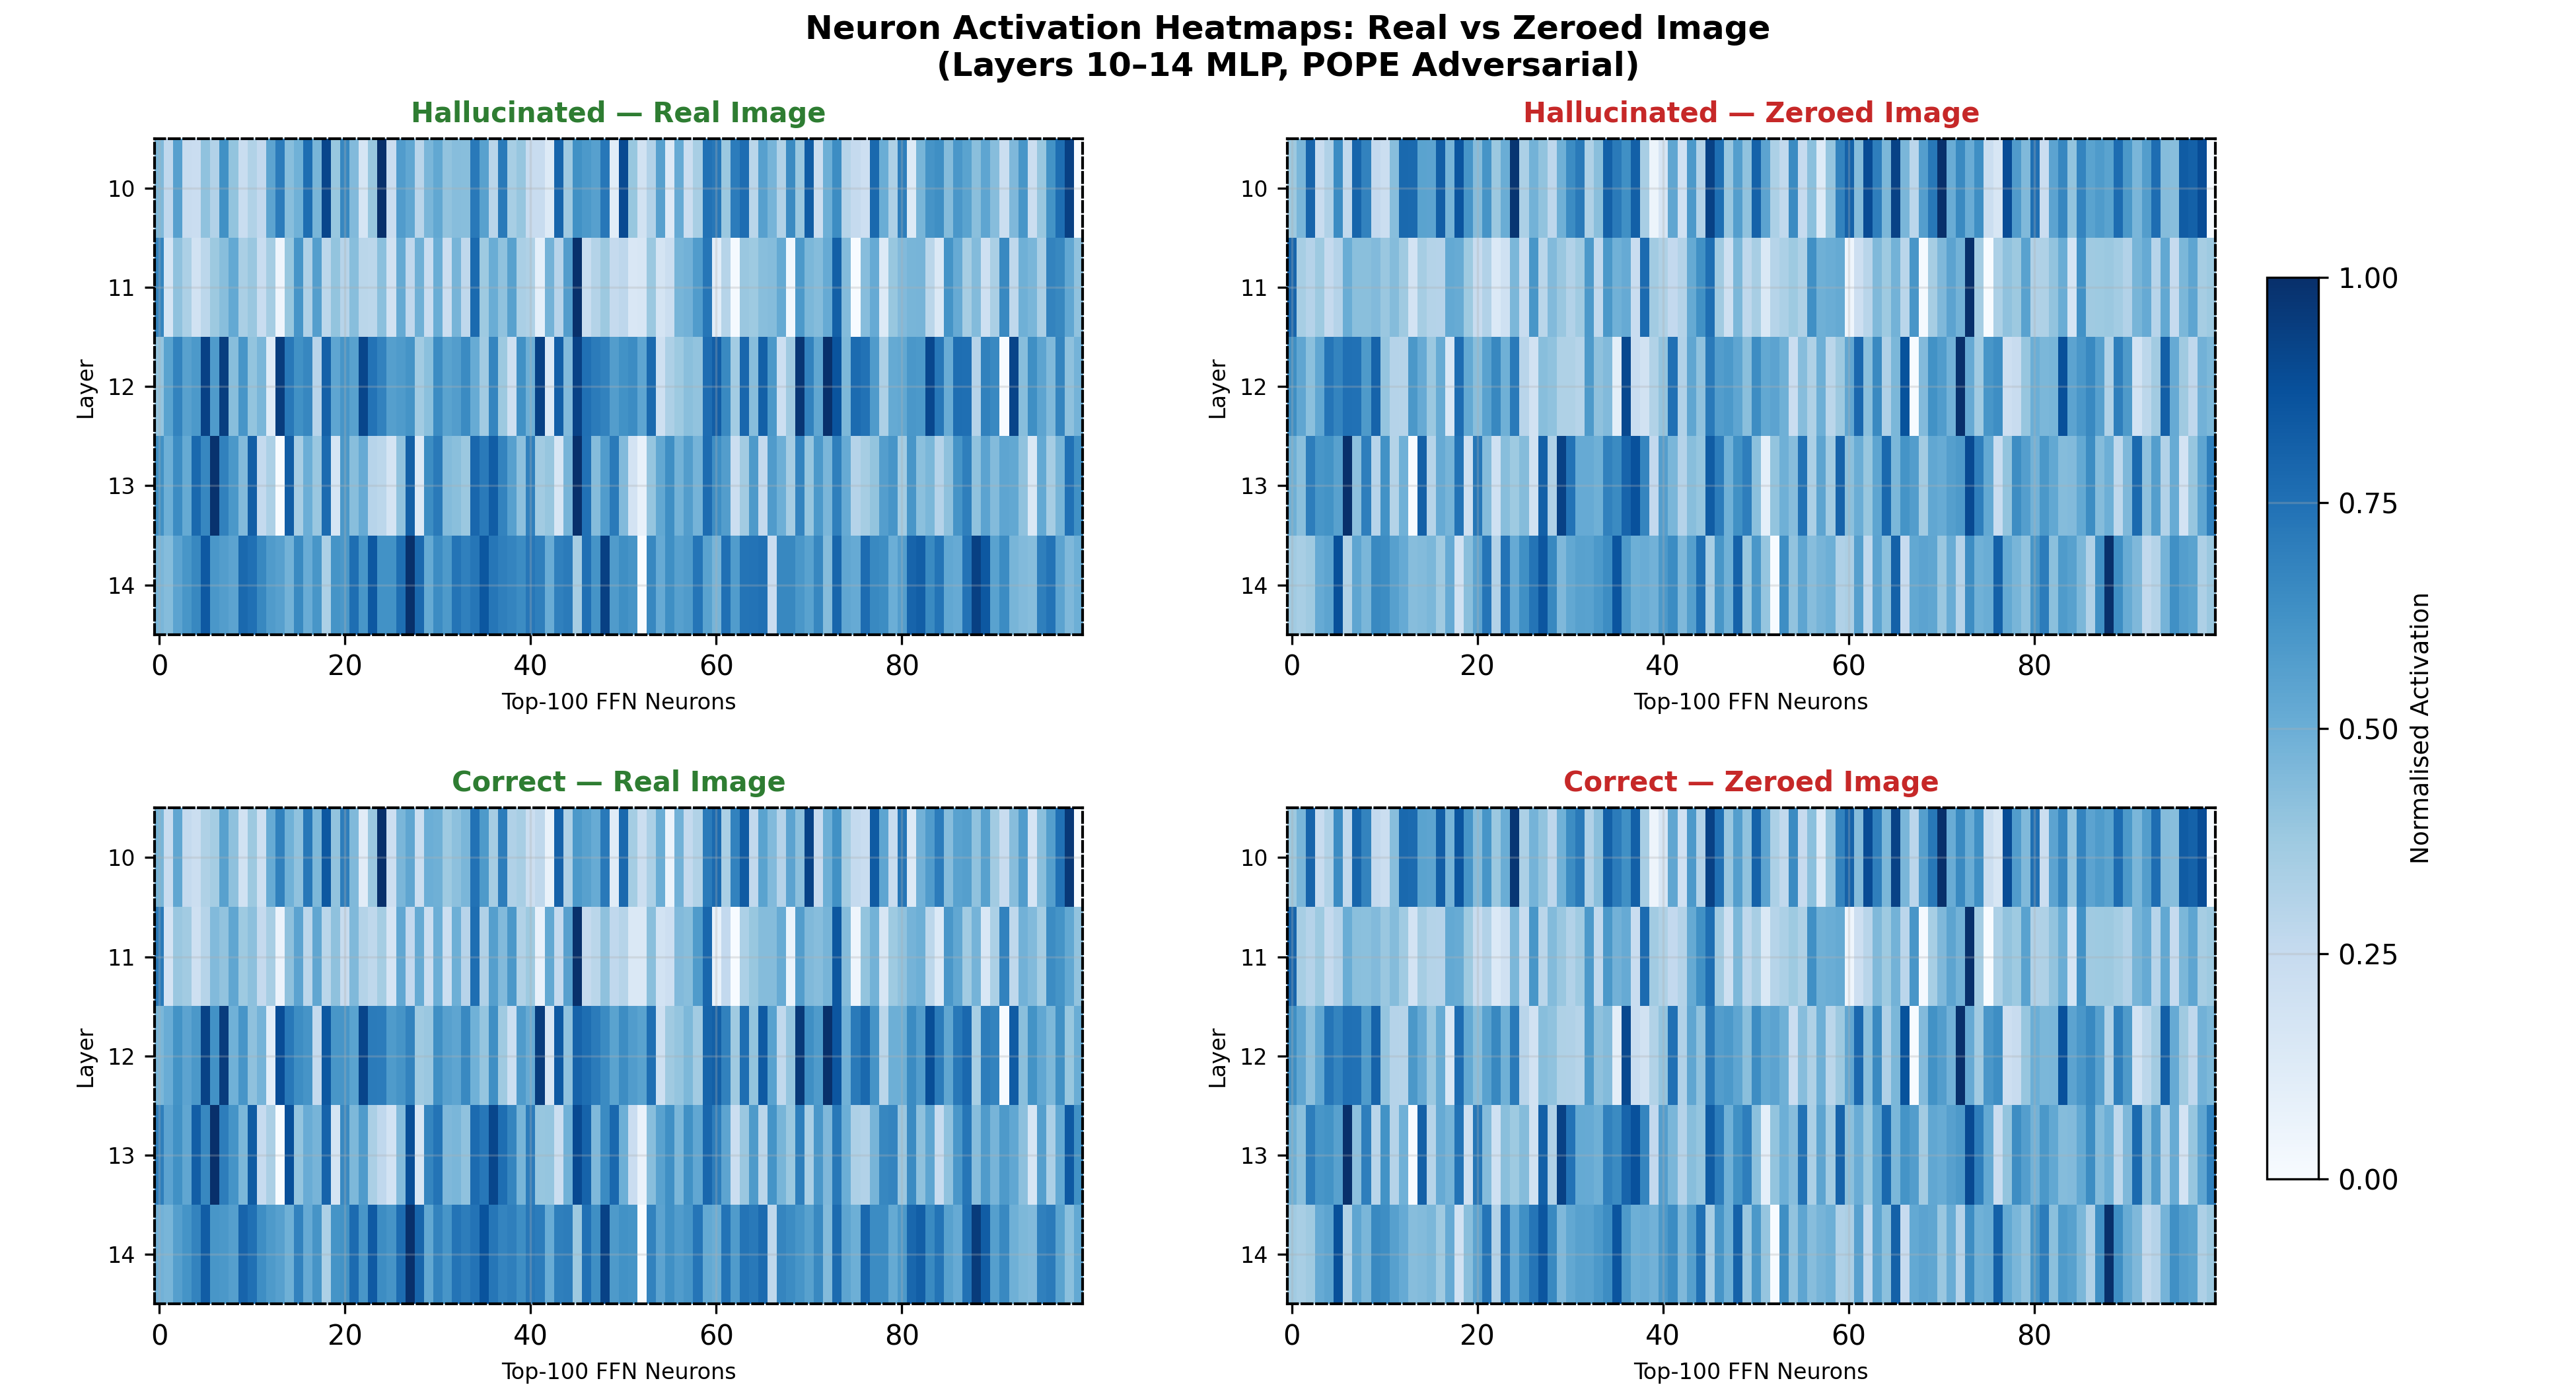
\includegraphics[width=\textwidth]{../EmberVLM/paper-template-Latest/figures/va_ablation_neuron_heatmap.png}
    \caption{\textbf{Neuron activation heatmaps.} \textbf{Top:} For hallucinated cases, activation patterns are nearly identical with and without the image, indicating generation from language priors. \textbf{Bottom:} For correctly grounded cases, activations change substantially when the image is removed, demonstrating reliance on actual visual content.}
    \label{fig:embervlm_neuron}
\end{figure}

\subsection{Combined Visual Absence Score}
The final visual absence probability for a given token combines both pathways:
\begin{equation}
    p_{\text{VA}} = \lambda \cdot p_{\text{neuron}} + (1-\lambda) \cdot s_{\text{logit}}
    \label{eq:va_combined}
\end{equation}
where $\lambda{=}0.5$ balances internal representation confidence against output distribution consistency.

\subsection{Type-Aware Intervention}
Using a heuristic dictionary of visually sensitive keywords (objects, colors, spatial relations), sensitive tokens face a strict hallucination threshold ($p_{\text{VA}} \geq 0.6$), while non-visual tokens face a looser boundary ($p_{\text{VA}} \geq 0.8$). Tokens exceeding their respective thresholds receive a severe logit penalty, forcing the model to select a more visually grounded alternative.

\subsection{Temporal Burst Detection}
Since hallucinations often occur in cascading clusters, the VA Refiner maintains a sliding-window temporal memory of recent $p_{\text{VA}}$ scores. If the moving average exceeds a predefined burst threshold, the refiner escalates from soft penalty to hard block (token logit $= -\infty$) and dampens the output distribution to break generative momentum.

\subsection{Mission Uncertainty Calibration}
After a full sequence is generated, the system aggregates $p_{\text{VA}}$ scores for all visually sensitive tokens. If the average absence score falls within a critical boundary, a system-level uncertainty flag is raised. Rather than prepending conversational caveats to the output, this flag signals the downstream autonomous controller that the current visual--tactical alignment is low-confidence, allowing the system to request a secondary camera angle or defer to human operator judgment. This transforms the VA Refiner from a pure text-generation mechanism into a systems-level reliability signal.

\subsection{Complete VA Refiner Inference Procedure}

Algorithm~\ref{alg:va_refiner} formalizes the full per-token intervention logic, integrating dual-view scoring, type-aware thresholding, and temporal burst detection into the decoding loop.

\begin{algorithm}[htbp]
\small
\caption{Visual Absence (VA) Refiner: per-token hallucination detection and logit intervention.}
\label{alg:va_refiner}
\begin{algorithmic}[1]
\Require Logits $L_{\text{vis}}$ (with image), $L_{\text{ablated}}$ (image ablated),
\Statex \hspace{\algorithmicindent} mid-decoder FFN activations $\mathbf{A}_{10:14}$,
\Statex \hspace{\algorithmicindent} thresholds $p^{\text{vis}}_{\text{VA}}{=}0.6$, $p^{\text{nonvis}}_{\text{VA}}{=}0.8$,
\Statex \hspace{\algorithmicindent} burst window $B$, burst threshold $\beta$, combination weight $\lambda{=}0.5$
\Ensure Adjusted logits $L_{\text{out}}$, system uncertainty flag
\State $s_{\text{logit}} \leftarrow 1.0 - \tanh(|L_{\text{vis}} - L_{\text{ablated}}|)$ \hfill\Comment{Eq.~\ref{eq:va_logit}}
\State $p_{\text{neuron}} \leftarrow \text{ContinuousMLP}(\text{top-}128(\mathbf{A}_{10:14}))$
\State $p_{\text{VA}} \leftarrow \lambda \cdot p_{\text{neuron}} + (1-\lambda) \cdot s_{\text{logit}}$ \hfill\Comment{Eq.~\ref{eq:va_combined}}
\State Append $p_{\text{VA}}$ to sliding window $W_{\text{burst}}$ of length $B$
\If{$\mathrm{mean}(W_{\text{burst}}) > \beta$} \Comment{hallucination burst}
    \State $L_{\text{out}} \leftarrow -\infty$; dampen output distribution
    \State \textbf{raise} system uncertainty flag; \Return $L_{\text{out}}$
\EndIf
\State sensitive $\leftarrow$ IsVisuallySensitive(current token, keyword dictionary)
\State threshold $\leftarrow$ $p^{\text{vis}}_{\text{VA}}$ if sensitive else $p^{\text{nonvis}}_{\text{VA}}$
\If{$p_{\text{VA}} \geq$ threshold}
    \State $L_{\text{out}} \leftarrow L_{\text{vis}} - \text{SeverePenalty}(\text{top-}k\text{ ungrounded candidates})$
\Else
    \State $L_{\text{out}} \leftarrow L_{\text{vis}}$ \Comment{no intervention needed}
\EndIf
\State \Return $L_{\text{out}}$
\end{algorithmic}
\end{algorithm}

\section{Four-Stage Training Curriculum}
\label{sec:embervlm_training_curriculum}

EmberVLM is trained through four supervised stages, each targeting a distinct capability, as illustrated in Figure~\ref{fig:embervlm_stages}. Training datasets are summarized in Table~\ref{tab:embervlm_datasets}, and hyperparameters in Table~\ref{tab:embervlm_hyperparams}.

\begin{figure}[!htb]
    \centering
    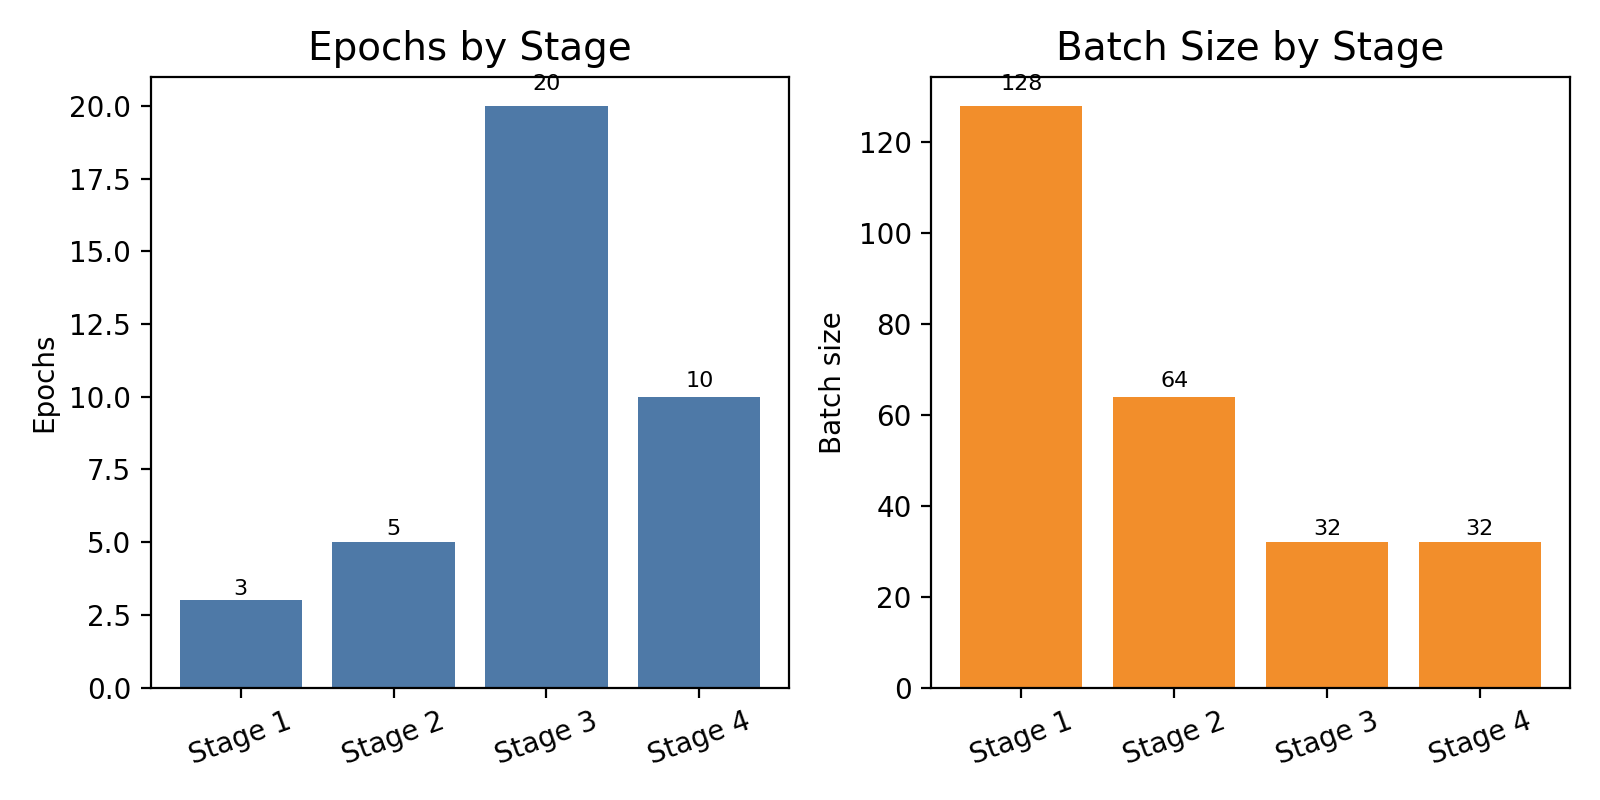
\includegraphics[width=\textwidth]{../EmberVLM/paper-template-Latest/figures/fig_training_stages.png}
    \caption{\textbf{EmberVLM four-stage training curriculum.} Stage~1 freezes both backbones and trains only the Fusion Module for visual-language alignment. Stage~2 unfreezes the language backbone for instruction tuning. Stage~3 re-freezes the backbone and trains the Reasoning Head for robot fleet selection. Stage~4 trains the Reasoning Head via InfoNCE contrastive loss to align internal step-embeddings with procedurally generated chain-of-thought rationales.}
    \label{fig:embervlm_stages}
\end{figure}

\begin{table}[htbp]
\centering
\caption{\textbf{EmberVLM training datasets across all stages.}}
\label{tab:embervlm_datasets}
\begin{tabular}{llc}
\toprule
\textbf{Stage} & \textbf{Dataset} & \textbf{Epochs} \\
\midrule
\multirow{8}{*}{1: Alignment} & CC3M~\cite{sharma2018cc3m} & 10 \\
 & RefCOCO~\cite{yu2016refcoco} & 10 \\
 & VQA v2~\cite{VQA} & 10 \\
 & COCO Annotations~\cite{lin2014coco} & 10 \\
 & LLaVA~\cite{liu2023llava} & 10 \\
 & OK-VQA~\cite{marino2019okvqa} & 10 \\
 & A-OKVQA~\cite{schwenk2022aokvqa} & 10 \\
 & GQA~\cite{hudson2019gqa} & 10 \\
\midrule
2: Instruction Tuning & LLaVA Instruct 150K & 15 \\
\midrule
3: Task Adaptation & Robot Selection & 20 \\
\midrule
4: Latent CoT & Robot Selection (CoT) & 10 \\
\bottomrule
\end{tabular}
\end{table}

\begin{figure}[!htb]
    \centering
    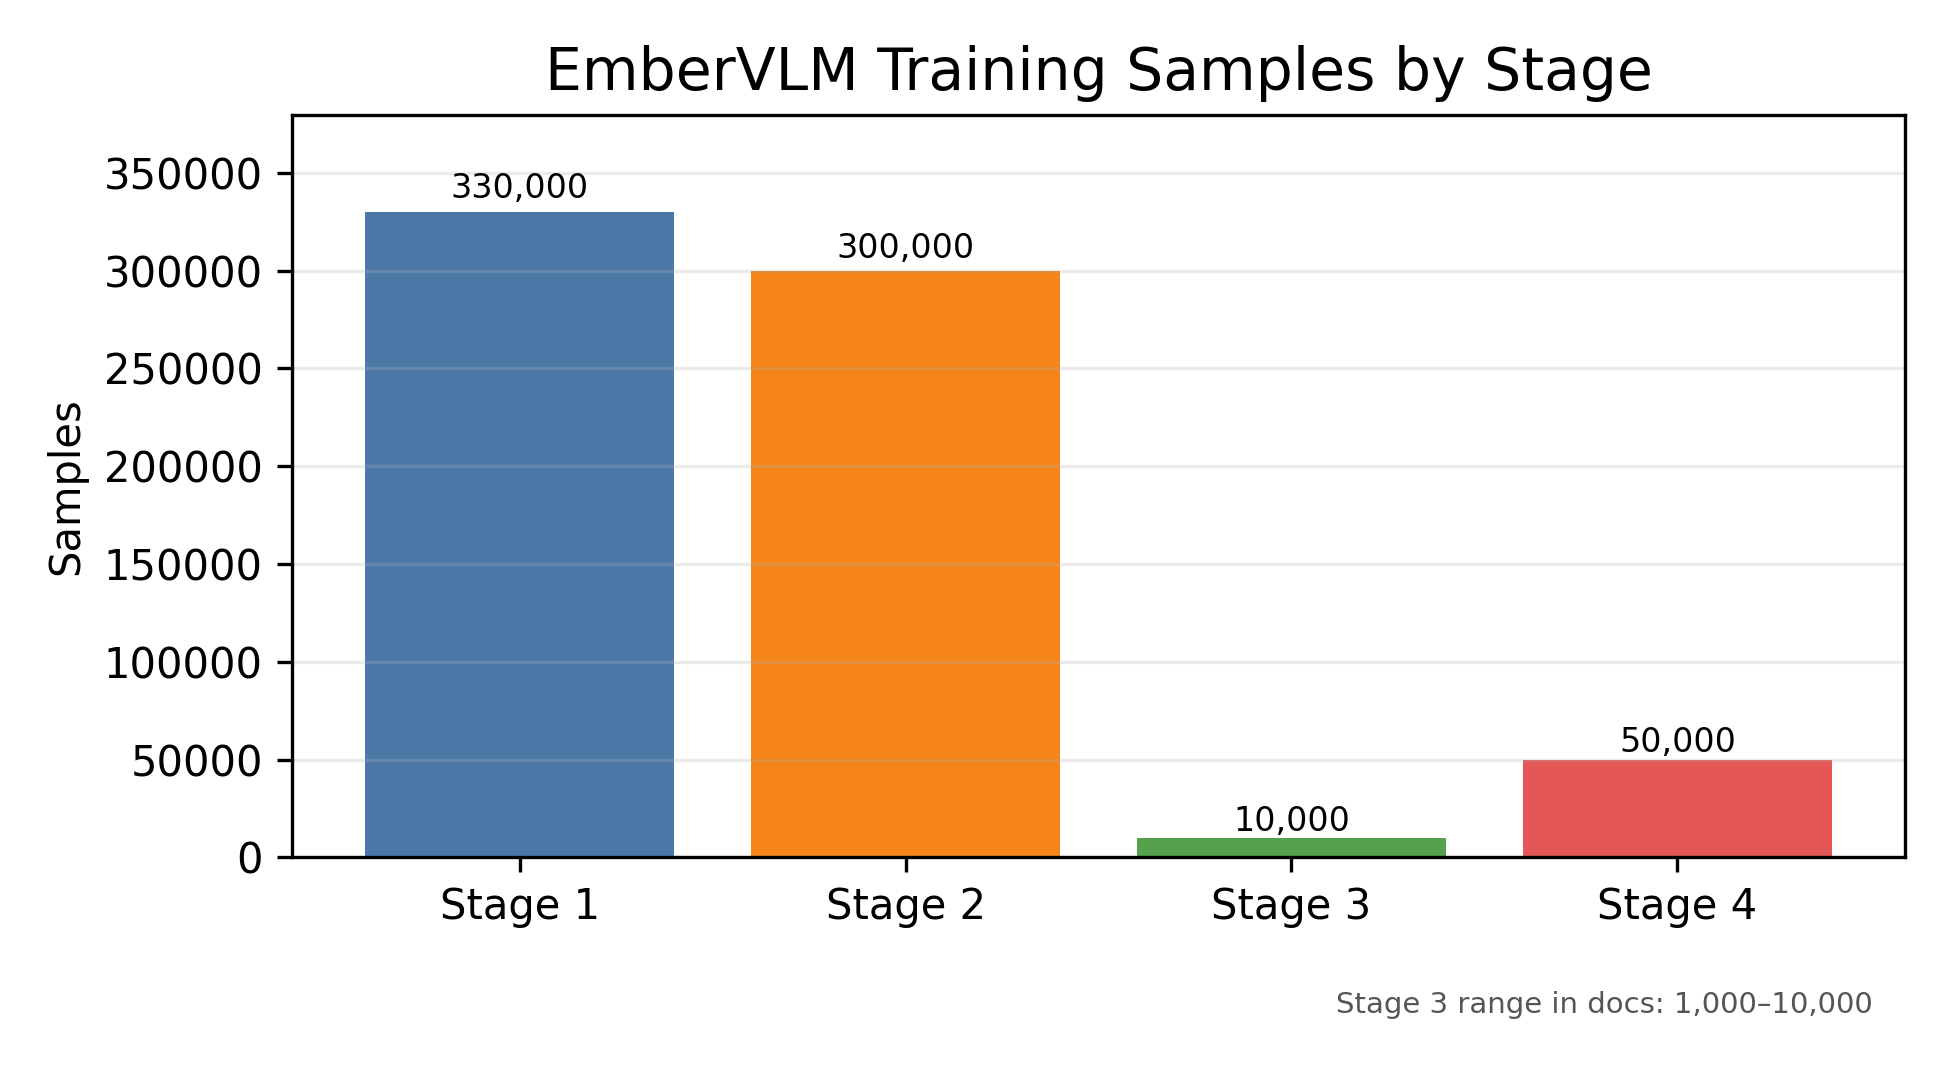
\includegraphics[width=\textwidth]{../EmberVLM/paper-template-Latest/figures/embervlm_stage_samples.png}
    \caption{\textbf{Representative training samples across stages.} Stage~1 alignment samples pair images with short captions. Stage~2 instruction tuning samples involve multi-turn visual dialogue. Stages~3--4 use structured robot-selection prompts with multi-label annotations and programmatic chain-of-thought rationales.}
    \label{fig:embervlm_stage_samples}
\end{figure}

\begin{table}[htbp]
\centering
\caption{\textbf{EmberVLM training hyperparameters by stage.}}
\label{tab:embervlm_hyperparams}
\resizebox{\textwidth}{!}{%
\begin{tabular}{lcccc}
\toprule
\textbf{Stage} & \textbf{LR} & \textbf{Eff. Batch} & \textbf{Max Seq.} & \textbf{Unfrozen Components} \\
\midrule
1: Alignment & $2\times10^{-4}$ & 256 & 512 & Fusion Module only \\
2: Instruction & $2\times10^{-4}$ & 256 & 512 & Fusion + Language Backbone \\
3: Task Adapt. & $1\times10^{-4}$ & 128 & 256 & Reasoning \& Action Head \\
4: Latent CoT & $1\times10^{-4}$ & 128 & 256 & Reasoning Head \\
\midrule
\multicolumn{5}{l}{\textit{All stages: AdamW ($\lambda_{\text{wd}}{=}10^{-2}$), cosine LR with 5\% warmup, bf16 mixed precision, 2$\times$A100.}} \\
\bottomrule
\end{tabular}%
}
\end{table}

\subsection{Stage 1: Visual-Language Alignment}
Vision and language backbones remain frozen; only the Fusion Module is actively trained. The model learns to map raw DINOv2 visual features into meaningful linguistic token space by predicting captions and answering standard visual queries across eight diverse datasets. This stage establishes the multimodal grounding capability without modifying the pretrained language or vision representations.

Figure~\ref{fig:stage1_heatmap} visualizes how text-to-patch attention evolves across training checkpoints during Stage 1. At the start of training (top row), attention is diffuse and unstructured. By mid-training (middle row), the model begins concentrating attention on semantically relevant regions consistent with the caption. By the end of Stage 1 (bottom row), attention is sharply localized to the salient scene elements described in the caption, confirming that the Fusion Module has learned to ground linguistic concepts in specific image patches.

\begin{figure}[!htb]
    \centering
    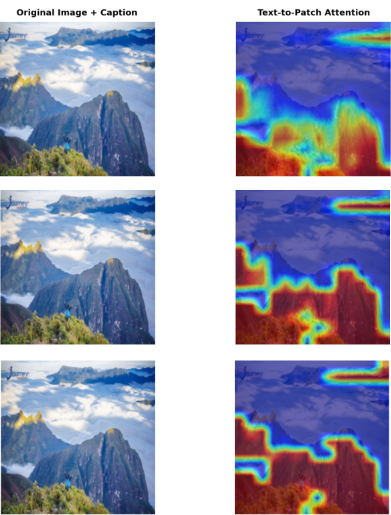
\includegraphics[width=0.85\linewidth]{heatmap_stage1.png}
    \caption{\textbf{Text-to-patch attention progression during Stage 1 alignment training.} Each row shows a training checkpoint (early, mid, late). The left column shows the input image with its associated caption; the right column shows the corresponding text-to-patch attention heatmap. Warm colors (red/yellow) indicate high attention weight on image patches. As training progresses, diffuse initial attention concentrates onto the semantically relevant regions of the scene, demonstrating the Fusion Module's acquisition of cross-modal visual grounding.}
    \label{fig:stage1_heatmap}
\end{figure}

\subsection{Stage 2: Multimodal Instruction Tuning}
The vision encoder remains frozen, but both the Fusion Module and the Language Backbone are fully unfrozen and fine-tuned end-to-end on LLaVA Instruct 150K. This enables the model to interpret nuanced human instructions and engage in multi-turn visual dialogue grounded in image content. Unfreezing the backbone in Stage 2 is the primary source of adaptable capacity in EmberVLM's training.

\subsection{Stage 3: Robot Fleet Selection}
The standard autoregressive head is bypassed, and the Reasoning and Action Head is unfrozen and trained with cross-entropy loss for Top-$K$ robot classification on the Robot Selection dataset. The backbone is re-frozen in this stage to prevent catastrophic forgetting of the instruction-tuning knowledge acquired in Stage 2.

\subsection{Stage 4: Latent Chain-of-Thought Integration}
Rather than predicting explicit CoT text tokens (which would add autoregressive latency at inference time), the Reasoning Head is trained to align its internal step-embeddings with procedurally generated Chain-of-Thought rationales using an InfoNCE contrastive loss ($\tau{=}0.07$):
\begin{equation}
    \mathcal{L}_{\text{CoT}} = -\log \frac{\exp(\mathrm{sim}(\mathbf{h}_{\text{reason}}, \mathbf{r}_{\text{CoT}})/\tau)}{\sum_{j}\exp(\mathrm{sim}(\mathbf{h}_{\text{reason}}, \mathbf{r}_j)/\tau)}
\end{equation}
Rationales are generated programmatically via a fixed rule-based template, requiring no external teacher model or human annotation:
\begin{verbatim}
"Scene analysis: [scene_description].
 Environmental condition: [condition].
 Required capability: [capability].
 Recommended robot type: [type].
 Reasoning: [rule-based justification]."
\end{verbatim}
Templates are instantiated from scene labels, environmental tags, and robot capability requirements from the dataset annotation. By training the head to align its \emph{internal embeddings} with CoT rationales rather than generating them token-by-token, EmberVLM gains deductive transparency without any inference-time latency penalty.

\section{Dynamic Tiered Memory Management}
\label{sec:embervlm_tiered_memory}

Figure~\ref{fig:embervlm_edge} shows the edge deployment scenario targeted by EmberVLM. Rather than pinning the entire 164M-parameter architecture in active compute memory, EmberVLM employs a dynamic tiered memory management strategy.

\begin{figure}[!htb]
    \centering
    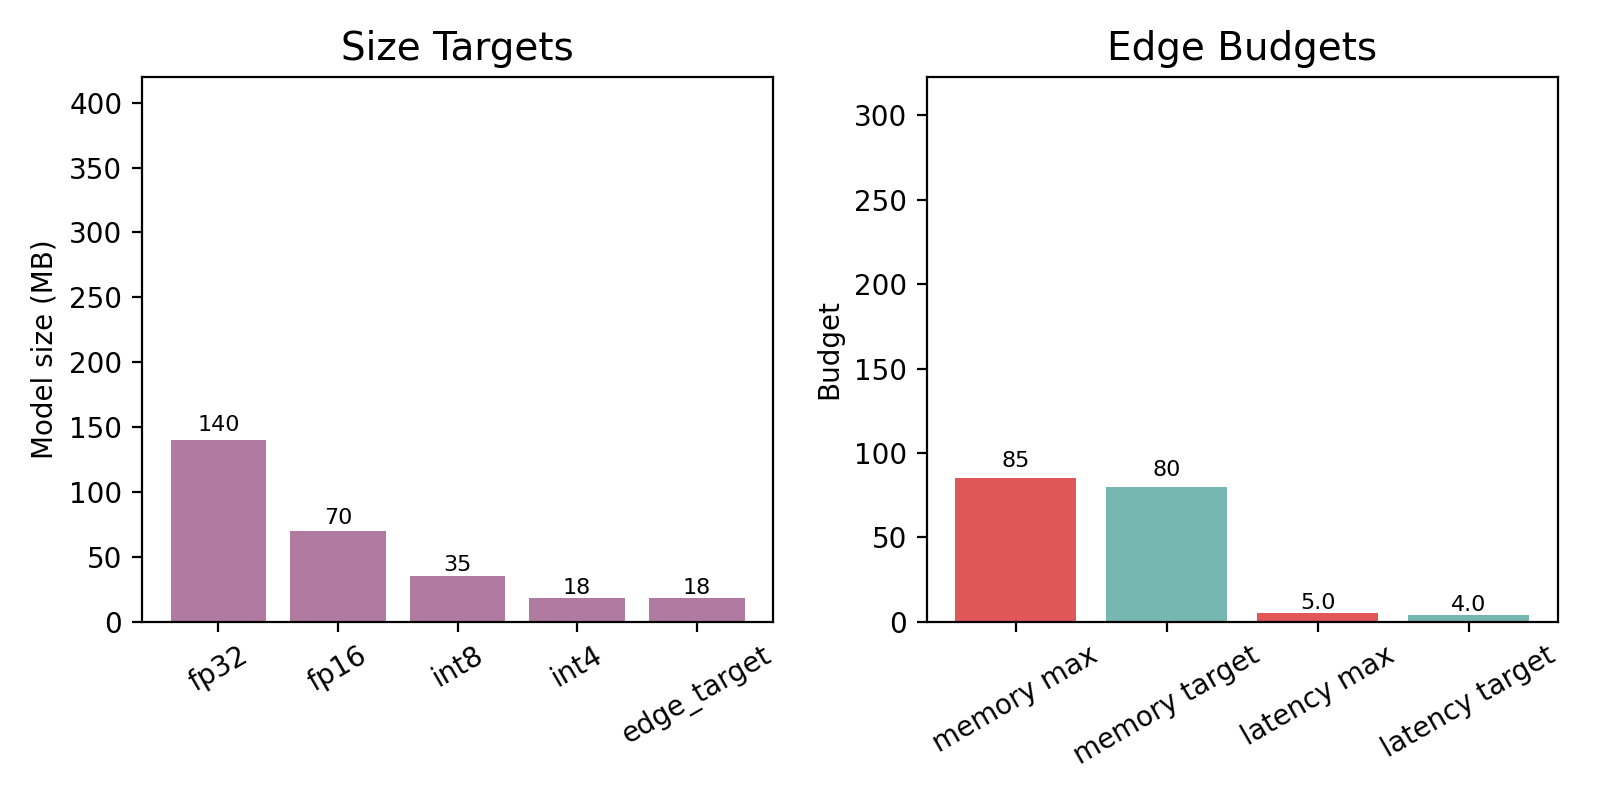
\includegraphics[width=0.9\linewidth]{../EmberVLM/paper-template-Latest/figures/fig_edge_targets.png}
    \caption{\textbf{Target edge deployment environments.} EmberVLM is designed for CPU-only hardware platforms such as the AMD Ryzen 3 4100 (3.80~GHz, 32~GB RAM, no discrete GPU), representative of resource-constrained field units used in emergency response, autonomous robotics, and remote sensing applications.}
    \label{fig:embervlm_edge}
\end{figure} The lightweight scope detector and the $512 \times 576$ memory matrix are permanently pinned to the primary compute device (total: $\sim$1.2~MB + scope detector parameters). For historically seen instances where the scope detector registers high confidence, the system directly retrieves contextual biases from memory without loading the full parametric model.

On AMD Ryzen 3 4100 (3.80 GHz, 32 GB RAM, no GPU), the full EmberVLM stack (Model + VA Refiner + Memory) operates at 5.22~ms per sample, consuming $<$800~MB RAM. For comparison, InternVL3-1B requires a discrete GPU with 1{,}978~MB VRAM and achieves only 1{,}566~ms per sample on the same hardware, making it categorically unsuitable for the target deployment regardless of its benchmark scores.

\section{Carbon Footprint Analysis}
\label{sec:embervlm_carbon}

\begin{table}[htbp]
\centering
\caption{\textbf{Training carbon emissions (CodeCarbon-measured).} All values are measured, not estimated. Training on 2$\times$A100 GPUs.}
\label{tab:embervlm_emissions}
\resizebox{\textwidth}{!}{%
\begin{tabular}{lrrc}
\toprule
\textbf{Stage} & \textbf{Duration} & \textbf{Emissions (kg CO$_2$eq)} & \textbf{\% of Total} \\
\midrule
Stage 1: Alignment     & 50 h (5 epochs)  & 16.6513 & 65.6\% \\
Stage 2: Instruction   & 40 h (13 epochs) & 8.6545  & 34.1\% \\
Stage 3: Robot Sel.    & $\approx$20 min  & 0.0046  & 0.02\% \\
Stage 4: Reasoning     & $\approx$10 min  & 0.0062  & 0.02\% \\
\midrule
\textbf{Total} & $\approx$90 h & \textbf{25.3166} & 100\% \\
\bottomrule
\end{tabular}%
}
\end{table}

Total measured training emissions across all stages are 25.3~kg CO$_2$eq, approximately equivalent to driving 100~km in an average gasoline car, and more than 21{,}000$\times$ less than GPT-3's estimated 552 tonnes CO$_2$eq~\cite{patterson2021carbon}. By constraining trainable parameters to 40M and completing all alignment and instruction tuning within approximately 90 hours on dual A100s, EmberVLM demonstrates that mission-critical capable multimodal AI can be trained sustainably. This positions low-carbon training not merely as a byproduct of efficiency but as a first-class design objective.

Carbon emissions were measured using CodeCarbon~\cite{codecarbon} integrated directly into the training loop. Measurements record actual power consumption of the 2$\times$A100 GPU cluster (hardware power draw via NVML), CPU, and memory, multiplied by the carbon intensity of the Taiwan electricity grid (approximately 0.509~kg~CO$_2$eq/kWh during the measurement period). All figures in Table~\ref{tab:embervlm_emissions} are \emph{measured}, not estimated from FLOPs or parameter counts.

        \chapter{Experiments and Results}
\label{cha:experiments}

\section{Experimental Setup}
\label{sec:exp_setup}

\subsection{Hardware and Software}
All EmberVLM training runs are conducted on 2$\times$NVIDIA A100 GPUs with BFloat16 (bf16) mixed precision. Edge deployment inference is evaluated on an AMD Ryzen 3 4100 4-Core Processor (3.80 GHz), 32 GB RAM, no discrete GPU, the actual target deployment hardware. All baseline models are evaluated on the same hardware for fair comparison. Per-sample latency is computed as total wall-clock time over the complete evaluation set divided by the number of samples.

\subsection{Evaluation Protocol}
For classification benchmarks (Top-N Robot Selection, VERI-Emergency, GEO-Bench-VLM), accuracy and F1 scores are computed using the official dataset evaluation protocols. For hallucination evaluation, the POPE benchmark~\cite{li2023pope} is used across three splits (Random, Popular, Adversarial), covering 9{,}000 samples total. The full POPE evaluation is preferred over subset evaluations to ensure statistical reliability of the 7pp absolute reduction claim.

\subsection{Baseline Models}
The following baselines are evaluated:
\begin{itemize}
    \item \textbf{InternVL3-1B} (938.2M parameters): requires discrete GPU, 1{,}978~MB VRAM.
    \item \textbf{MobileVLM\_V2-1.7B} (1{,}674.1M parameters): requires GPU.
    \item \textbf{SmolVLM-256M} (256.5M parameters): requires GPU.
    \item \textbf{SmolVLM2-256M} (256.5M parameters): requires GPU.
    \item \textbf{EmberVLM NoMem}: EmberVLM without episodic memory (parametric generation only).
    \item \textbf{EmberVLM}: full model with ONLINE\_UPDATE memory mode.
\end{itemize}

\subsection{Robot Selection Dataset}

Figure~\ref{fig:robot_distribution} shows the class distribution and co-occurrence structure of the Robot Selection dataset used for primary evaluation. The 500-sample dataset exhibits significant class imbalance: Drone (226 labels), Humanoid (243), and Robot with Legs (247) account for the majority of annotations, while Underwater Robot (64) and Robot with Wheels (81) are substantially under-represented. This imbalance directly explains the per-class F1 variance observed in Section~\ref{sec:exp_mission_critical}.

\begin{figure}[!htb]
    \centering
    \begin{minipage}[t]{0.48\linewidth}
        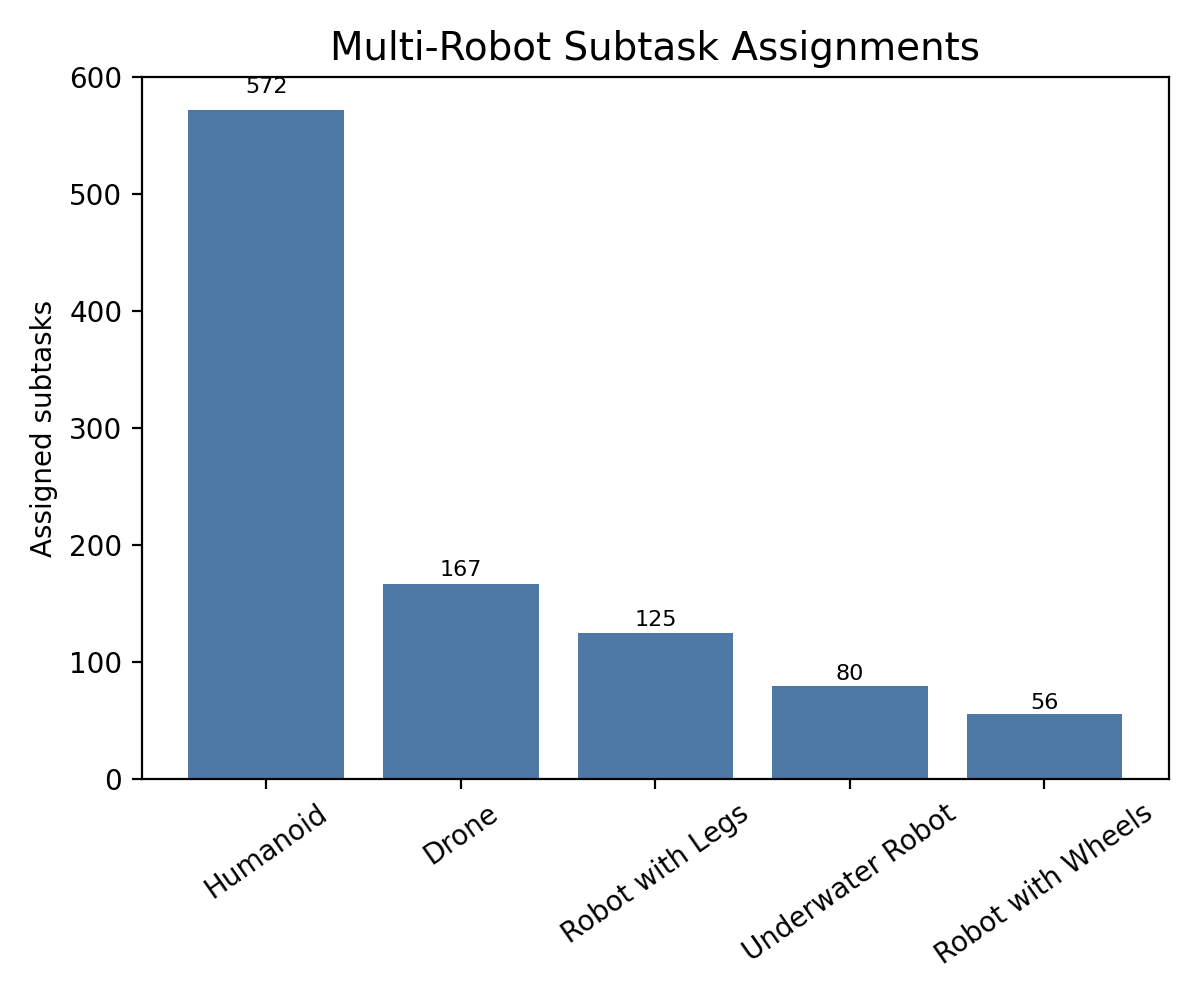
\includegraphics[width=\linewidth]{../EmberVLM/paper-template-Latest/figures/fig_multi_robot_distribution.png}
        \centering{(a) Multi-label class distribution}
    \end{minipage}\hfill
    \begin{minipage}[t]{0.48\linewidth}
        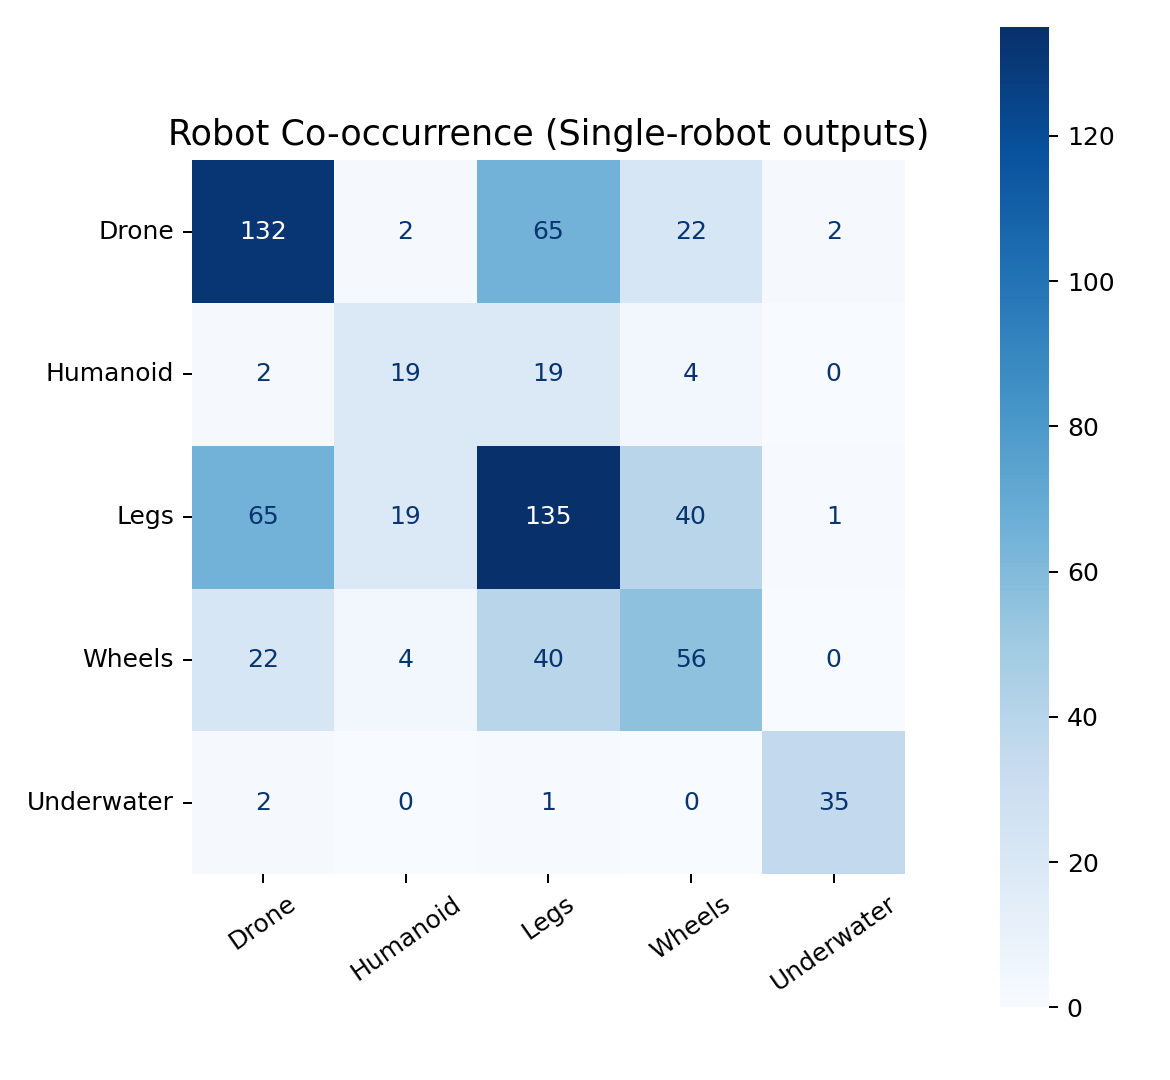
\includegraphics[width=\linewidth]{../EmberVLM/paper-template-Latest/figures/fig_robot_cooccurrence.png}
        \centering{(b) Class co-occurrence matrix}
    \end{minipage}
    \caption{\textbf{Robot Selection dataset statistics.} (a) Per-class label counts across train/val/test splits. Underwater Robot and Robot with Wheels are the most scarce classes, contributing to high prediction variance on the validation split. (b) Class co-occurrence matrix showing which robot types are frequently annotated together in the same scenario.}
    \label{fig:robot_distribution}
\end{figure}

Figure~\ref{fig:input_distribution} shows the input text length distribution and single-output class distribution across the dataset, providing context for the sequence length hyperparameters (256 tokens for Stages~3--4) and the multi-label structure of the evaluation task.

\begin{figure}[!htb]
    \centering
    \begin{minipage}[t]{0.48\linewidth}
        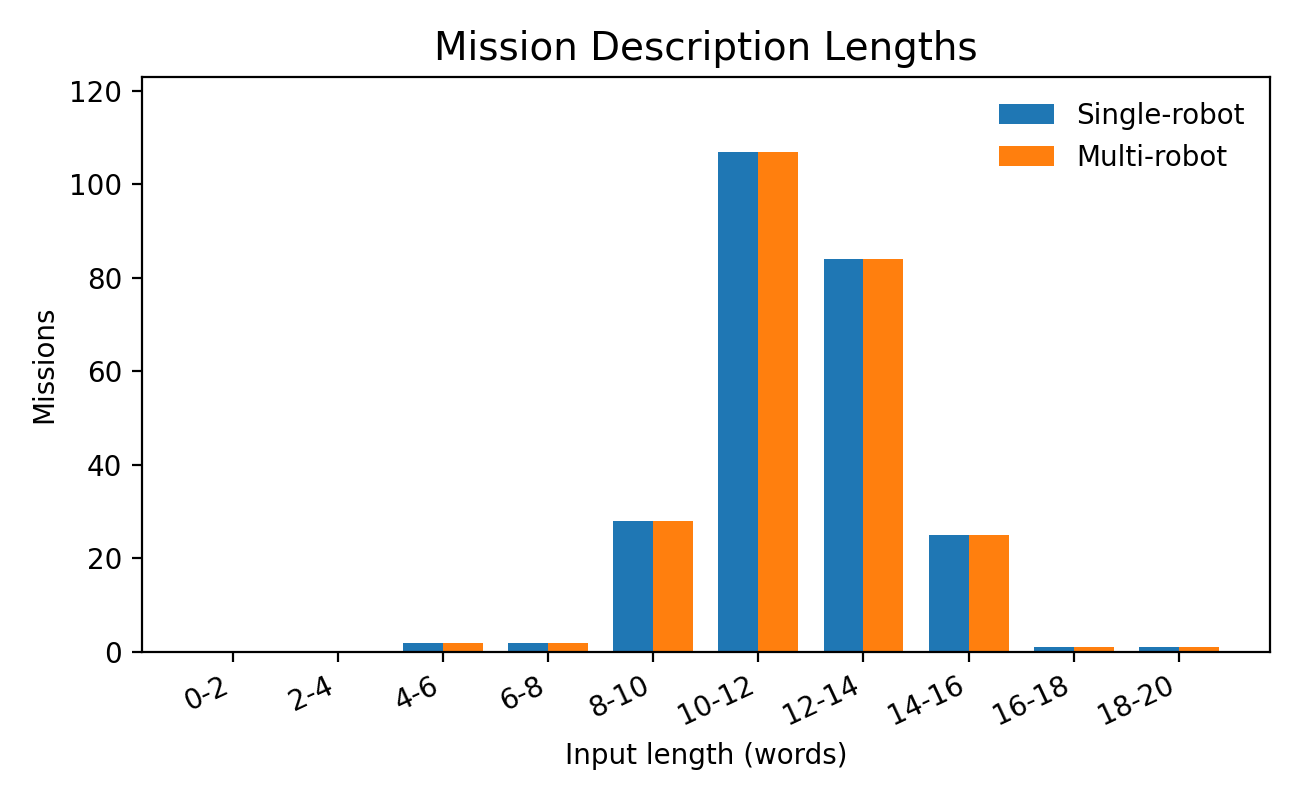
\includegraphics[width=\linewidth]{../EmberVLM/paper-template-Latest/figures/fig_input_length_distribution.png}
        \centering{(a) Input token length distribution}
    \end{minipage}\hfill
    \begin{minipage}[t]{0.48\linewidth}
        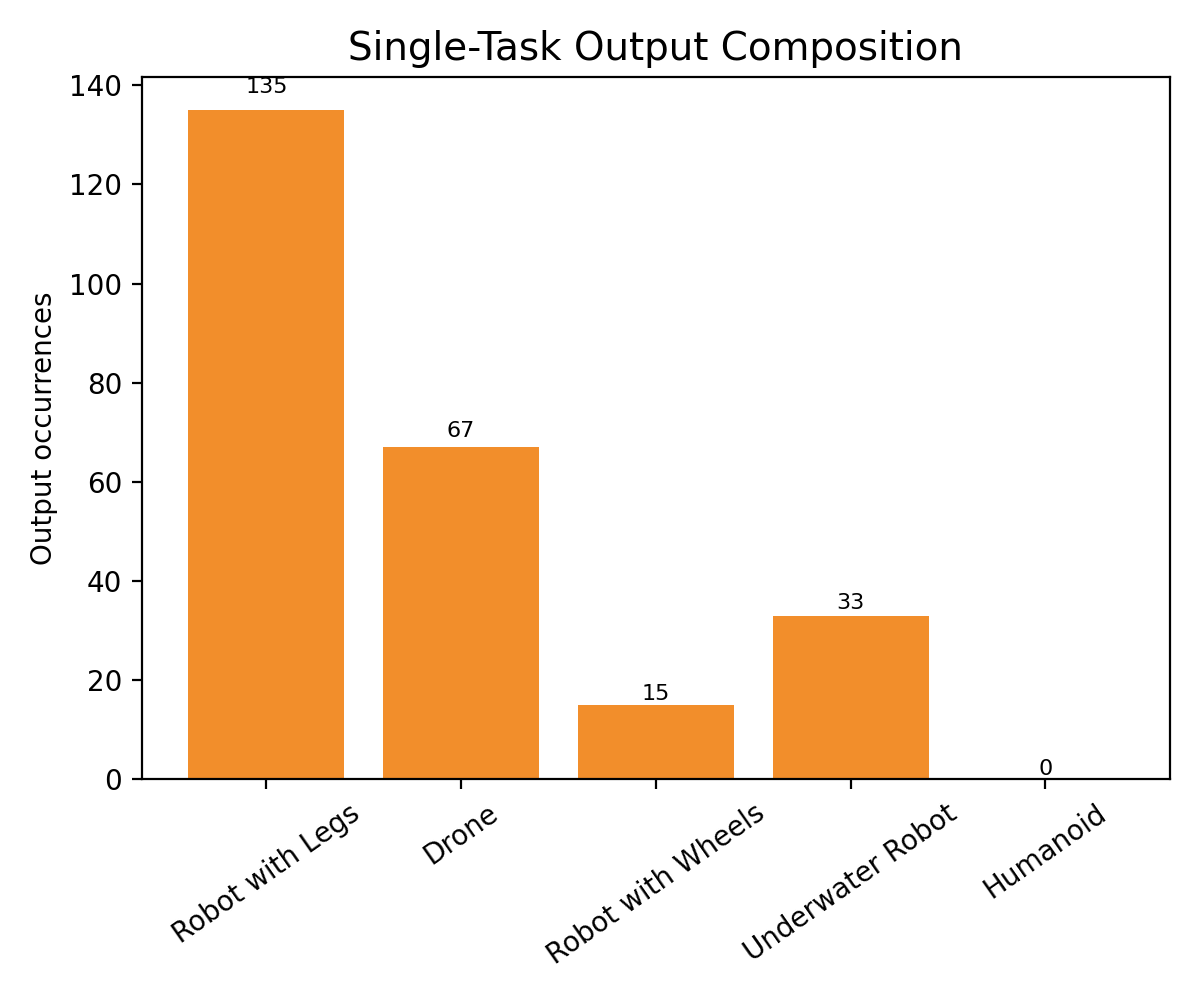
\includegraphics[width=\linewidth]{../EmberVLM/paper-template-Latest/figures/fig_single_output_distribution.png}
        \centering{(b) Single-label output distribution}
    \end{minipage}
    \caption{\textbf{Robot Selection input and output statistics.} (a) Input scenario descriptions are predominantly 20--80 tokens long, well within the 256-token maximum sequence length used in Stages~3--4. (b) The single-label output class distribution confirms that multi-robot scenarios are common, validating the multi-label evaluation protocol.}
    \label{fig:input_distribution}
\end{figure}

\section{Mission-Critical Benchmark Results}
\label{sec:exp_mission_critical}

\begin{table}[htbp]
\centering
\caption{\textbf{Performance on mission-critical visual recognition benchmarks.} Time(s) = total wall-clock over the full evaluation set on the AMD Ryzen 3 4100 CPU. OverRx / UnderRx = over/under-reaction rates (lower UnderRx is safer).}
\label{tab:mission_critical}
\resizebox{\textwidth}{!}{
\begin{tabular}{l|ccc|ccc|cc}
\toprule
\multirow{2}{*}{\textbf{Model}} & \multicolumn{3}{c|}{\textbf{Top-$N$ Robot Selection}} & \multicolumn{3}{c|}{\textbf{VERI-Emergency}} & \multicolumn{2}{c}{\textbf{GEO-Bench-VLM}} \\
\cmidrule(lr){2-4}\cmidrule(lr){5-7}\cmidrule(lr){8-9}
 & ExactAcc. & Macro-F1 & Time(s) & Acc. & OverRx & UnderRx & Acc. & Time(s) \\
\midrule
InternVL3-1B     & 0.0550 & 0.1380 & \textbf{187.5}  & \textbf{0.6310} & 0.6600 & \textbf{0.0650} & 0.3810 & 1051.7 \\
MobileVLM\_V2-1.7B & 0.0960 & 0.2294 & 271.6 & 0.5350 & 0.4700 & 0.4600 & 0.1580 & \textbf{175.0} \\
SmolVLM-256M     & 0.0000 & 0.1391 & 557.4 & 0.4950 & 0.0100 & 1.0000 & 0.2066 & 2001.4 \\
SmolVLM2-256M    & 0.0000 & 0.2254 & 513.9 & 0.5000 & \textbf{0.0000} & 1.0000 & 0.2383 & 1834.7 \\
\midrule
EmberVLM NoMem   & 0.0960 & 0.2350 & 3641.8 & 0.4700 & 0.7700 & 0.2900 & 0.2086 & 6244.3 \\
\textbf{EmberVLM}& \textbf{0.2100} & \textbf{0.4200} & 2381.9 & \textbf{0.6400} & 0.5200 & 0.1400 & \textbf{0.7200} & 2247.7 \\
\bottomrule
\end{tabular}
}
\end{table}

\subsection{Top-N Robot Selection}

Figure~\ref{fig:robot_subtasks} shows the subtask count distribution within the dataset, confirming that the majority of scenarios require selecting between two and four robot types simultaneously, establishing the multi-label nature of the primary evaluation task.

\begin{figure}[!htb]
    \centering
    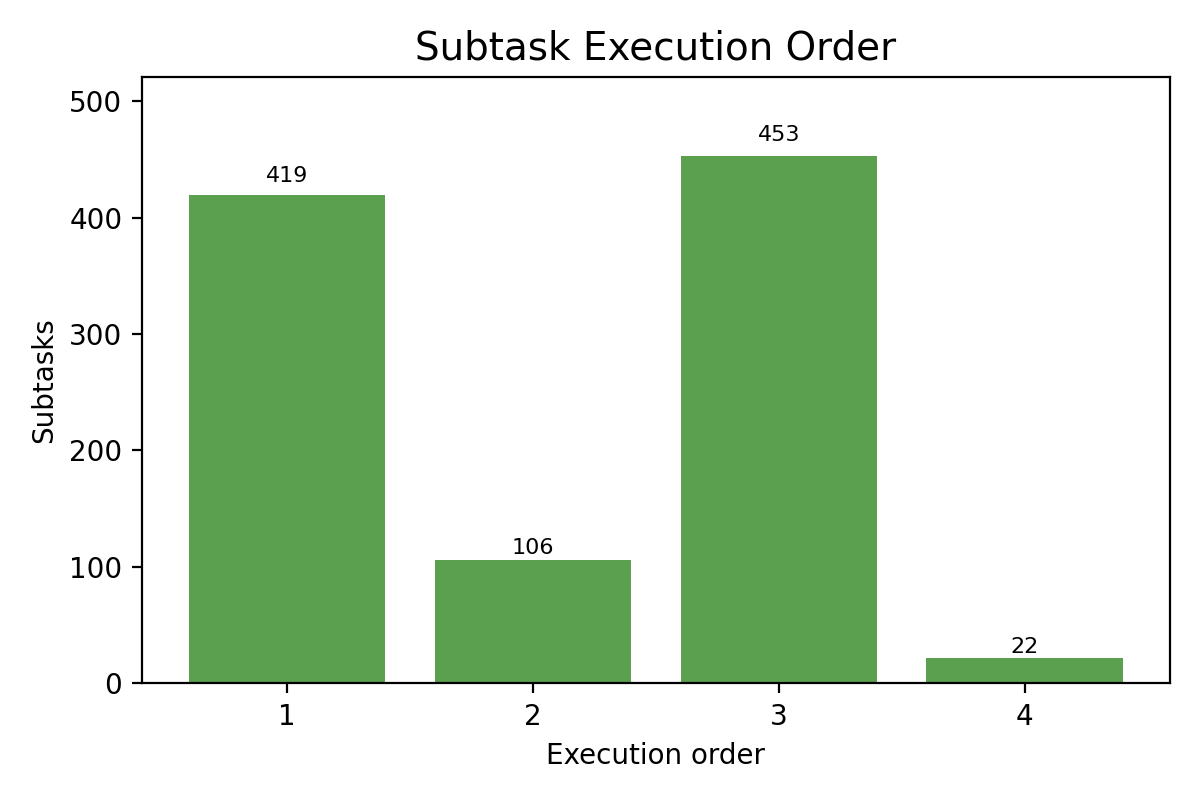
\includegraphics[width=0.65\linewidth]{../EmberVLM/paper-template-Latest/figures/fig_subtask_count_distribution.png}
    \caption{\textbf{Distribution of required robot types per scenario.} Most scenarios require two or more robot types, confirming that single-label classification is insufficient and validating the multi-label evaluation protocol using Macro-F1 and Jaccard similarity.}
    \label{fig:robot_subtasks}
\end{figure}

Table~\ref{tab:mission_critical} shows that without episodic memory, EmberVLM NoMem degrades into a near single-class predictor (Exact Accuracy = 0.0960, Macro-F1 = 0.2350). Table~\ref{tab:robot_selection_detail} provides the full ablation on the 103-sample validation split.

\begin{table}[htbp]
\centering
\caption{\textbf{Robot fleet selection ablation.} 103-sample validation split. ECE: lower is better ($\downarrow$); all others: higher is better ($\uparrow$).}
\label{tab:robot_selection_detail}
\begin{tabular}{lccc}
\toprule
\textbf{Metric} & \textbf{NoMemory} & \textbf{YesMemory} & \textbf{Abs. $\Delta$} \\
\midrule
Validation accuracy & 0.0971 & 0.5437 & $+$0.4466 \\
Macro precision & 0.0194 & 0.2811 & $+$0.2617 \\
Macro recall & 0.2000 & 0.3458 & $+$0.1458 \\
Macro F1 & 0.0354 & 0.2970 & $+$0.2616 \\
ECE $\downarrow$ & 0.3409 & 0.1849 & $-$0.1560 \\
Multi-robot exact match & 0.0097 & 0.0874 & $+$0.0777 \\
Multi-robot Jaccard & 0.0097 & 0.2961 & $+$0.2864 \\
\bottomrule
\end{tabular}
\end{table}

Without memory, the model heavily over-indexes on the ``Robot-with-Wheels'' class (Recall = 1.0, F1 = 0.177) while entirely failing on Drone, Underwater Robot, Humanoid, and Robot-with-Legs (F1 = 0.0 for all). With episodic memory, the model successfully discriminates across multiple morphologies: Drone (F1 = 0.6667, Precision = 0.5054, Recall = 0.9792) and Underwater Robot (F1 = 0.8182, Precision = 0.9000, Recall = 0.7500) both achieve strong results. Humanoid and Robot-with-Legs remain at F1 = 0.0 for both variants, correctly attributed to their extreme scarcity in the 103-sample validation split rather than a failure of memory conditioning.

\begin{table}[htbp]
\centering
\caption{\textbf{Top-N Robot Selection dataset split statistics.} Per-class sample counts across train, validation, and test splits. Classes are imbalanced, with Underwater Robot and Robot with Wheels being the least frequent.}
\label{tab:robot_dataset_stats}
\begin{tabular}{lrrrr}
\toprule
\textbf{Class} & \textbf{Train} & \textbf{Val} & \textbf{Test} & \textbf{Total} \\
\midrule
Drone & 148 & 53 & 25 & 226 \\
Underwater Robot & 41 & 13 & 10 & 64 \\
Humanoid & 166 & 46 & 31 & 243 \\
Robot with Wheels & 54 & 15 & 12 & 81 \\
Robot with Legs & 166 & 45 & 36 & 247 \\
\midrule
\textbf{Total} & 331 & 103 & 66 & 500 \\
\bottomrule
\end{tabular}
\end{table}

\subsection{VERI-Emergency}

On VERI-Emergency, EmberVLM achieves the highest overall accuracy (0.6400) and a competitive UnderRx of 0.1400. InternVL3-1B achieves a lower UnderRx (0.0700) but at substantially higher latency (per-sample latency $\approx$ 10.2~s vs. EmberVLM's 23~ms on the same hardware) and requiring GPU hardware that is not available in the target deployment context. For edge deployment, the combination of accuracy, UnderRx, latency, and hardware requirements must all be evaluated jointly rather than optimizing UnderRx alone.

SmolVLM and SmolVLM2 achieve very low OverRx ($\leq$0.01) but achieve UnderRx of 1.0, meaning they never flag genuine emergency signals, rendering them useless for safety-critical deployment despite their low false alarm rates.

\subsection{GEO-Bench-VLM}

EmberVLM achieves 0.7200, the highest accuracy among all evaluated models. InternVL3-1B achieves only 0.3772, and SmolVLM variants score below 0.25. The strong geospatial performance is attributed to episodic memory: geospatial incident scenes benefit strongly from retrieval of visually similar historical episodes. Generic pretrained representations alone cannot replicate this, given the domain-specific nature of disaster imagery.

\section{General Multimodal Benchmarks}
\label{sec:exp_general}

\begin{table}[htbp]
\centering
\caption{\textbf{General multimodal benchmarks and inference efficiency.}}
\label{tab:general_benchmarks}
\begin{tabular}{lcc}
\toprule
\textbf{Metric} & \textbf{No Memory} & \textbf{With Memory} \\
\midrule
Coherence aggregate score & 13.1 & \textbf{17.1} \\
GQA VQA~\cite{hudson2019gqa} & 10.0\% & 10.0\% \\
UniBench~\cite{altahan2024unibench} & 7.0\% & \textbf{8.0\%} \\
SugarCrepe~\cite{hsieh2023sugarcrepe} & 14.0\% & \textbf{16.0\%} \\
\midrule
Extra FLOPs per step & \textbf{0} & $\sim$0.3--0.6M \\
Episodic memory RAM & \textbf{0} & $\sim$1.2 MB \\
\bottomrule
\end{tabular}
\end{table}

Table~\ref{tab:general_benchmarks} shows consistent improvements across general multimodal benchmarks with episodic memory: a 30\% relative improvement in coherence aggregate score (13.1 $\rightarrow$ 17.1), a 14.3\% relative gain on SugarCrepe (14.0\% $\rightarrow$ 16.0\%), and a 1-point absolute gain on UniBench. GQA accuracy is unchanged at 10.0\%, which reflects the fixed parametric capacity for raw visual question answering.

EmberVLM's lower absolute scores on GQA (9.40\%) and SugarCrepe (15.30\%) compared to larger models reflect the inherent capacity constraint of a 164M total parameter model with only 40M trainable parameters. The quality-to-compute ratio of 17.1/1.03 versus 13.1/1.0 confirms that episodic memory is an optimal strategy for scaling reasoning without violating edge constraints.

Figure~\ref{fig:radar_mission} presents a five-axis normalized benchmark radar spanning mission-critical performance, general visual reasoning, and latency efficiency. EmberVLM leads on the two axes that govern edge deployment viability: mission-critical score (${\approx}0.95$) and latency efficiency (1.0, since it is the fastest model on CPU). InternVL3-1B leads the three general-benchmark axes at $5.7\times$ the parameter count but scores near zero on latency efficiency, confirming it is categorically unsuitable for edge deployment regardless of its VQA capability.

\begin{figure}[!htb]
\centering
\begin{tikzpicture}
\definecolor{emberred}{RGB}{210,60,40}
\definecolor{emberorange}{RGB}{230,140,40}
\definecolor{emberteal}{RGB}{40,160,140}
\definecolor{emberpurple}{RGB}{120,60,160}
\definecolor{embergray}{RGB}{130,130,130}
\foreach \ring in {
  {(0.0,0.6)--(0.5706,0.1854)--(0.3527,-0.4854)--(-0.3527,-0.4854)--(-0.5706,0.1854)--cycle},
  {(0.0,1.2)--(1.1413,0.3708)--(0.7053,-0.9708)--(-0.7053,-0.9708)--(-1.1413,0.3708)--cycle},
  {(0.0,1.8)--(1.7119,0.5562)--(1.0580,-1.4562)--(-1.0580,-1.4562)--(-1.7119,0.5562)--cycle},
  {(0.0,2.4)--(2.2825,0.7416)--(1.4107,-1.9416)--(-1.4107,-1.9416)--(-2.2825,0.7416)--cycle}
}{ \draw[gray!28, thin] \ring; }
\foreach \ep in {
  (0.0,2.4),(2.2825,0.7416),(1.4107,-1.9416),
  (-1.4107,-1.9416),(-2.2825,0.7416)
}{ \draw[gray!40, thin] (0,0) -- \ep; }
\node[font=\tiny,gray,anchor=west] at (0.06,0.60) {.25};
\node[font=\tiny,gray,anchor=west] at (0.06,1.20) {.50};
\node[font=\tiny,gray,anchor=west] at (0.06,1.80) {.75};
\node[font=\small,anchor=south,align=center] at (0.0,3.22)
  {\textbf{MC Score}\\[-2pt]{\scriptsize\textit{(Top-N$\cdot$VERI$\cdot$GEO)}}};
\node[font=\small,anchor=west,align=left] at (3.062,0.995)
  {\textbf{GQA}\\[-2pt]{\scriptsize\textit{(Visual Reasoning)}}};
\node[font=\small,anchor=north west,align=left] at (1.893,-2.605)
  {\textbf{SugarCrepe}\\[-2pt]{\scriptsize\textit{(Compositionality)}}};
\node[font=\small,anchor=north east,align=right] at (-1.893,-2.605)
  {\textbf{Coherence}\\[-2pt]{\scriptsize\textit{(avg GQA+Wino+Sugar)}}};
\node[font=\small,anchor=east,align=right] at (-3.062,0.995)
  {\textbf{Latency Eff.}\\[-2pt]{\scriptsize\textit{(CPU$\uparrow$)}}};
% InternVL3-1B [0.639, 1.000, 1.000, 1.000, 0.003]
\draw[emberteal,line width=1.3pt]
  (0.0,1.5336)--(2.2825,0.7416)--(1.4107,-1.9416)--(-1.4107,-1.9416)--(-0.0068,0.0022)--cycle;
% MobileVLM [0.588, 0.000, 0.533, 0.387, 0.006]
\draw[emberorange,line width=1.3pt]
  (0.0,1.4112)--(0.0,0.0)--(0.7513,-1.0343)--(-0.5459,-0.7511)--(-0.0137,0.0044)--cycle;
% SmolVLM-256M [0.530, 0.394, 0.582, 0.540, 0.006]
\draw[emberpurple,line width=1.3pt]
  (0.0,1.2720)--(0.8990,0.2921)--(0.8212,-1.1301)--(-0.7614,-1.0484)--(-0.0137,0.0044)--cycle;
% SmolVLM2-256M [0.588, 0.074, 0.586, 0.433, 0.004]
\draw[embergray,line width=1.3pt]
  (0.0,1.4112)--(0.1686,0.0548)--(0.8270,-1.1382)--(-0.6104,-0.8401)--(-0.0091,0.0030)--cycle;
% EmberVLM [0.952, 0.165, 0.165, 0.279, 1.000]
\fill[emberred!18]
  (0.0,2.2848)--(0.3763,0.1223)--(0.2327,-0.3204)--(-0.6696,-0.9408)--(-2.2825,0.7416)--cycle;
\draw[emberred,line width=2.2pt]
  (0.0,2.2848)--(0.3763,0.1223)--(0.2327,-0.3204)--(-0.6696,-0.9408)--(-2.2825,0.7416)--cycle;
\node[anchor=north west, font=\scriptsize] at (1.6, 3.5) {
  \begin{tikzpicture}
    \draw[emberred,    line width=2.2pt] (0,0.80)--(0.45,0.80);
    \node[right, font=\scriptsize] at (0.48,0.80) {\textbf{EmberVLM} \textit{(w/ Ep.\ Mem.)}};
    \draw[emberteal,   line width=1.3pt] (0,0.45)--(0.45,0.45);
    \node[right, font=\scriptsize] at (0.48,0.45) {InternVL3-1B};
    \draw[emberorange, line width=1.3pt] (0,0.10)--(0.45,0.10);
    \node[right, font=\scriptsize] at (0.48,0.10) {MobileVLM\_V2-1.7B};
    \draw[emberpurple, line width=1.3pt] (0,-0.25)--(0.45,-0.25);
    \node[right, font=\scriptsize] at (0.48,-0.25) {SmolVLM-256M};
    \draw[embergray,   line width=1.3pt] (0,-0.60)--(0.45,-0.60);
    \node[right, font=\scriptsize] at (0.48,-0.60) {SmolVLM2-256M};
  \end{tikzpicture}
};
\end{tikzpicture}
\caption{\textbf{Five-axis normalized benchmark radar.} EmberVLM (red, filled) leads on MC Score (${\approx}0.95$, collapsing Top-N Robot Selection, VERI-Emergency, and GEO-Bench) and dominates the Latency Efficiency axis (inverted: min\_latency/latency, so CPU-only EmberVLM = 1.0 and GPU baselines near zero). InternVL3-1B sweeps the three general-benchmark axes but scores near zero on latency efficiency, confirming it is unsuitable for the target hardware despite its higher VQA accuracy. The \textbf{MC Score} and \textbf{Latency Efficiency} axes directly govern edge deployment viability.}
\label{fig:radar_mission}
\end{figure}

\section{Episodic Memory Ablation}
\label{sec:exp_memory_ablation}

Table~\ref{tab:memory_mode_ablation} presents the three-mode memory ablation across all mission-critical benchmarks: OFF, READ\-\_ONLY, and ONLINE\-\_UPDATE.

\begin{table}[htbp]
\centering
\caption{\textbf{Memory mode ablation across mission-critical benchmarks.}}
\label{tab:memory_mode_ablation}
\resizebox{\textwidth}{!}{%
\begin{tabular}{lccc}
\toprule
\textbf{Configuration} & \textbf{Robot Sel. (Macro-F1)} & \textbf{VERI (Acc.)} & \textbf{GEO (Acc.)} \\
\midrule
OFF & 0.0354 & 0.4700 & 0.2086 \\
READ\_ONLY & \textbf{0.2970} & 0.6200 & \textbf{0.7200} \\
ONLINE\_UPDATE & 0.2100 & \textbf{0.6400} & 0.7100 \\
\bottomrule
\end{tabular}%
}
\end{table}

READ\_ONLY leads on robot selection, confirming that the primary value of episodic memory is structured retrieval from a clean offline snapshot rather than online accumulation. ONLINE\_UPDATE achieves the lowest UnderRx on VERI-Emergency (0.215 vs. 0.285 for OFF), the most safety-critical metric, suggesting live writes help with rare or recently seen emergency signatures. GEO-Bench results are broadly flat across modes, consistent with the fixed-capacity ($K{=}512$) memory being diluted across a wider geospatial concept space.

Figure~\ref{fig:radar_memory} shows a per-class F1 radar chart comparing all three memory modes on the Top-N Robot Selection task. READ\_ONLY achieves the broadest per-class coverage. ONLINE\_UPDATE shows stronger recall on Underwater Robot (the scarcest class), suggesting that live writes improve handling of rare morphologies not well-represented in the frozen offline snapshot.

\begin{figure}[!htb]
\centering
\begin{tikzpicture}[scale=1.0]
\definecolor{emberred}{RGB}{210,60,40}
\definecolor{emberorange}{RGB}{230,140,40}
\definecolor{emberteal}{RGB}{40,160,140}
\def\R{2.2}
\foreach \r in {0.25,0.5,0.75,1.0}{
  \draw[gray!25, thin]
    ({(\R*\r)*sin(0)},   {(\R*\r)*cos(0)})   --
    ({(\R*\r)*sin(72)},  {(\R*\r)*cos(72)})  --
    ({(\R*\r)*sin(144)}, {(\R*\r)*cos(144)}) --
    ({(\R*\r)*sin(216)}, {(\R*\r)*cos(216)}) --
    ({(\R*\r)*sin(288)}, {(\R*\r)*cos(288)}) -- cycle;
}
\foreach \i in {0,1,2,3,4}{
  \draw[gray!45, thin] (0,0) --
    ({(\R)*sin(\i*72)}, {(\R)*cos(\i*72)});
}
\node[font=\tiny, gray, anchor=west] at (0.06, \R*0.5) {0.5};
\node[font=\scriptsize, anchor=south]      at ({(\R+0.3)*sin(0)},   {(\R+0.3)*cos(0)})   {Drone};
\node[font=\scriptsize, anchor=west]       at ({(\R+0.3)*sin(72)},  {(\R+0.3)*cos(72)})  {Underwater};
\node[font=\scriptsize, anchor=north west] at ({(\R+0.3)*sin(144)}, {(\R+0.3)*cos(144)}) {Humanoid};
\node[font=\scriptsize, anchor=north east] at ({(\R+0.3)*sin(216)}, {(\R+0.3)*cos(216)}) {Wheels};
\node[font=\scriptsize, anchor=east]       at ({(\R+0.3)*sin(288)}, {(\R+0.3)*cos(288)}) {Legs};
% OFF: 0.353, 0.091, 0.296, 0.152, 0.289
\draw[emberred, thick, fill=emberred!18]
  ({(\R*0.353)*sin(0)},  {(\R*0.353)*cos(0)})  --
  ({(\R*0.091)*sin(72)}, {(\R*0.091)*cos(72)}) --
  ({(\R*0.296)*sin(144)},{(\R*0.296)*cos(144)}) --
  ({(\R*0.152)*sin(216)},{(\R*0.152)*cos(216)}) --
  ({(\R*0.289)*sin(288)},{(\R*0.289)*cos(288)}) -- cycle;
% READ_ONLY: 0.310, 0.182, 0.329, 0.121, 0.342
\draw[emberteal, thick, fill=emberteal!18]
  ({(\R*0.310)*sin(0)},  {(\R*0.310)*cos(0)})  --
  ({(\R*0.182)*sin(72)}, {(\R*0.182)*cos(72)}) --
  ({(\R*0.329)*sin(144)},{(\R*0.329)*cos(144)}) --
  ({(\R*0.121)*sin(216)},{(\R*0.121)*cos(216)}) --
  ({(\R*0.342)*sin(288)},{(\R*0.342)*cos(288)}) -- cycle;
% ONLINE_UPDATE: 0.323, 0.197, 0.261, 0.168, 0.222
\draw[emberorange, thick, fill=emberorange!18]
  ({(\R*0.323)*sin(0)},  {(\R*0.323)*cos(0)})  --
  ({(\R*0.197)*sin(72)}, {(\R*0.197)*cos(72)}) --
  ({(\R*0.261)*sin(144)},{(\R*0.261)*cos(144)}) --
  ({(\R*0.168)*sin(216)},{(\R*0.168)*cos(216)}) --
  ({(\R*0.222)*sin(288)},{(\R*0.222)*cos(288)}) -- cycle;
\node[anchor=north west, font=\scriptsize] at (1.15, 2.85) {
  \begin{tikzpicture}
    \draw[emberred,    thick] (0,0.4)--(0.4,0.4);  \node[right, font=\scriptsize] at (0.42,0.4)  {OFF};
    \draw[emberteal,   thick] (0,0.0)--(0.4,0.0);  \node[right, font=\scriptsize] at (0.42,0.0)  {READ\_ONLY};
    \draw[emberorange, thick] (0,-0.4)--(0.4,-0.4);\node[right, font=\scriptsize] at (0.42,-0.4) {ONLINE\_UPDATE};
  \end{tikzpicture}
};
\end{tikzpicture}
\caption{\textbf{Per-class F1 radar chart across memory modes (Top-N Robot Selection).} READ\_ONLY achieves the broadest coverage overall. ONLINE\_UPDATE shows stronger per-class recall on the Underwater Robot axis, the scarcest class (13 validation samples), suggesting live writes partially address rare-morphology prediction.}
\label{fig:radar_memory}
\end{figure}

\section{Visual Absence Refiner Ablation}
\label{sec:exp_va_ablation}

\begin{table}[htbp]
\centering
\caption{\textbf{VA Refiner component ablation across all mission-critical benchmarks.} Memory mode = ONLINE\_UPDATE for all rows. $\downarrow$ = lower is better.}
\label{tab:va_ablation}
\resizebox{\textwidth}{!}{%
\begin{tabular}{lcccccc}
\toprule
 & \multicolumn{2}{c}{\textbf{Robot Selection}} & \multicolumn{2}{c}{\textbf{VERI-Emergency}} & \multicolumn{2}{c}{\textbf{GEO-Bench}} \\
\cmidrule(lr){2-3}\cmidrule(lr){4-5}\cmidrule(lr){6-7}
\textbf{VA Mode} & Macro-F1 & Jaccard & Acc. & UnderRx$\downarrow$ & Acc. & Time(s) \\
\midrule
Off (baseline) & \textbf{0.251} & \textbf{0.207} & \textbf{0.520} & 0.240 & 0.194 & 2302.9 \\
Logit only & 0.215 & 0.192 & 0.485 & 0.290 & \textbf{0.207} & 2576.4 \\
Neuron only & 0.217 & 0.198 & 0.475 & 0.320 & 0.201 & 2503.2 \\
\textbf{Full (logit + neuron)} & 0.219 & 0.185 & 0.480 & \textbf{0.270} & 0.202 & 2761.2 \\
\bottomrule
\end{tabular}%
}
\end{table}

Table~\ref{tab:va_ablation} shows that the VA Refiner has no statistically significant effect on the robot selection classification head, which uses a non-autoregressive MLP head bypassing the LM token generation pathway entirely. The Refiner's benefit is concentrated in generative outputs: on VERI-Emergency, the full mode achieves the lowest UnderRx (0.270 vs. 0.240 for VA-off), the most safety-critical metric. On GEO-Bench, the logit-only pathway improves accuracy by 1.3pp. The VA Refiner introduces 19\% additional inference time overhead at batch=1 (from 4.19~ms to 4.81~ms), a cost fully justified by the safety improvement in generative outputs.

Figure~\ref{fig:va_drop} illustrates the hallucination reduction achieved by the VA Refiner on the POPE Adversarial split.

\begin{figure}[!htb]
    \centering
    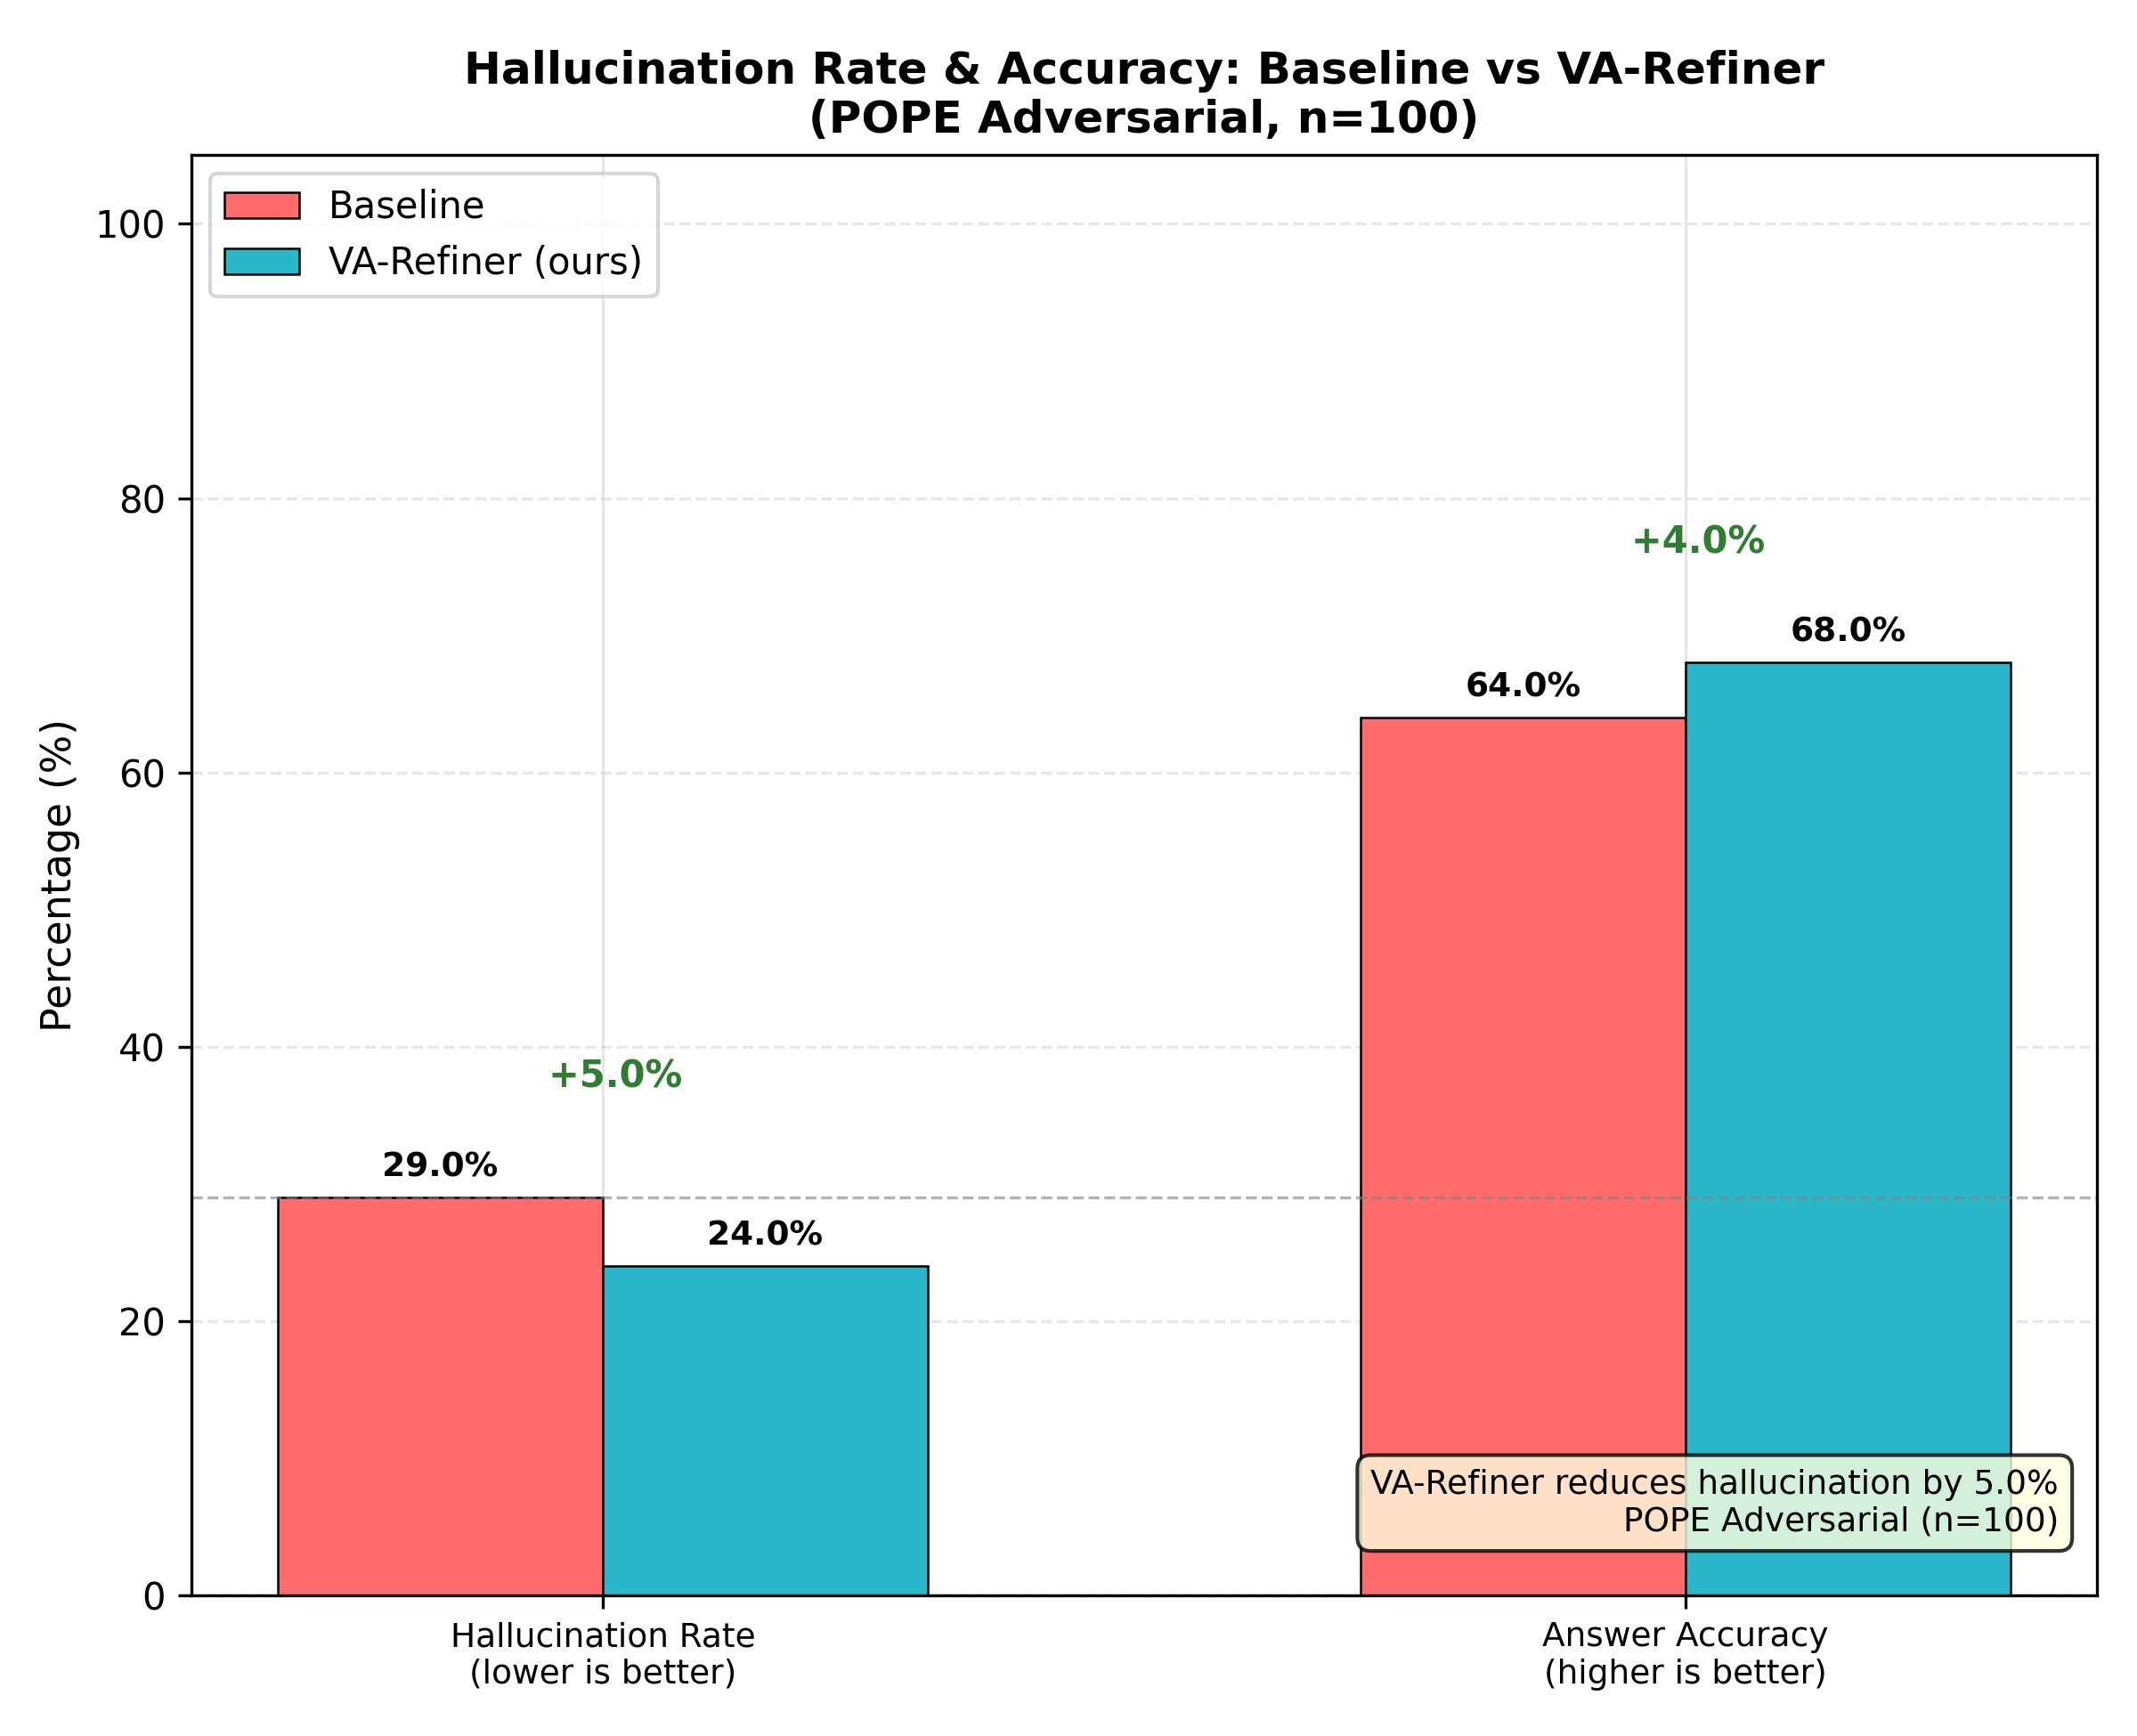
\includegraphics[width=0.75\linewidth]{../EmberVLM/paper-template-Latest/figures/va_ablation_hallucination_drop.png}
    \caption{\textbf{VA Refiner hallucination drop on POPE Adversarial split.} Each bar shows the hallucination rate before and after VA Refiner activation. EmberVLM achieves the largest absolute reduction ($-$7pp, from 29\% to 22\%), while SmolVLM2-256M also shows a substantial improvement ($-$3.47pp). InternVL3-1B and SmolVLM-256M show no benefit, consistent with their strong internal visual grounding.}
    \label{fig:va_drop}
\end{figure}

\begin{table}[htbp]
\centering
\caption{\textbf{POPE hallucination rates by split.} Evaluated on the complete 9{,}000-sample POPE dataset. $\Delta\downarrow$ = absolute hallucination rate reduction; lower is better.}
\label{tab:pope_results}
\scriptsize
\setlength{\tabcolsep}{3pt}
\begin{tabular}{lcc|cc|cc|cc}
\toprule
\textbf{Model} & Adv. & +VA & Pop. & +VA & Rand. & +VA & Overall & $\Delta\downarrow$ \\
\midrule
InternVL3-1B       & 13.73 & 13.73 & 8.73  & 8.73  & 2.27 & 2.27 & 8.24  & 0.00 \\
MobileVLM\_V2-1.7B & 6.93  & 5.87  & 6.53  & 5.73  & 6.67 & 5.53 & 6.71  & $-$1.00 \\
SmolVLM-256M       & 15.47 & 15.47 & 9.80  & 9.80  & 3.33 & 3.33 & 9.53  & 0.00 \\
SmolVLM2-256M      & 20.20 & 15.47 & 14.73 & 10.40 & 4.67 & 4.27 & 13.20 & $-$3.47 \\
\textbf{EmberVLM}  & 29.00 & 22.00 & 21.20 & 15.00 & 6.70 & 6.13 & 29.00 & \textbf{$-$7.00} \\
\bottomrule
\end{tabular}
\end{table}

The VA Refiner shows no benefit for InternVL3-1B and SmolVLM-256M; both already exhibit strong internal visual grounding, meaning their mid-decoder neurons are strongly modulated by visual input regardless of image presence. The Refiner's calibrated classifier is specific to SmolLM-135M's activation patterns. SmolVLM2-256M shows a 3.47pp improvement, suggesting partial cross-architecture transfer for models of similar compact scale. Evaluated on the full 9{,}000-sample POPE dataset, the $-$7pp reduction for EmberVLM is robust across all three splits (Adversarial: 29\%~$\rightarrow$~22\%; Popular: 21.2\%~$\rightarrow$~15.0\%; Random: 6.7\%~$\rightarrow$~6.13\%).

\section{Edge Deployment Latency Analysis}
\label{sec:exp_latency}

\begin{table}[htbp]
\centering
\caption{\textbf{CPU-only edge inference latency} on AMD Ryzen 3 4100. Full stack = Model + VA Refiner + Memory.}
\label{tab:latency}
\begin{tabular}{llcc}
\toprule
\textbf{Configuration} & \textbf{Batch} & \textbf{Latency (ms)} & \textbf{Samples/s} \\
\midrule
Model only & 1 & 4.19 & 238.4 \\
Model + VA & 1 & 4.81 & 207.9 \\
Model + Memory & 1 & 4.41 & 226.9 \\
\textbf{Model + VA + Memory} & \textbf{1} & \textbf{5.22} & \textbf{191.7} \\
\midrule
Model only & 16 & 159.8 & 100.1 \\
Model + VA + Memory & 16 & 135.5 & 118.1 \\
\bottomrule
\end{tabular}
\end{table}

At batch size 1 (the operational single-incident edge scenario), the full stack adds only 1.03~ms over model-only, a 24.6\% relative overhead that is negligible for discrete incident-response events. At batch size 16, the full stack is actually \emph{faster} than model-only (135.5~ms vs. 159.8~ms), because the memory retrieval replaces longer generative decoding paths in the batch.

\section{Mechanistic Analysis of Hallucinations}
\label{sec:exp_mechanistic}

The neuron activation heatmap analysis (Figure~\ref{fig:embervlm_neuron} in Chapter~\ref{cha:embervlm}) reveals the precise internal mechanism underlying object hallucination. For hallucinated tokens, mid-decoder neuron activation patterns in layers 10--14 remain highly symmetric regardless of whether visual input is present. These specific neurons fire independently of visual context, relying entirely on the language model's pretrained semantic priors to select a plausible-sounding token.

For correctly grounded tokens, the same neurons exhibit dramatically different activation patterns when the image is removed, confirming structural dependence on actual visual content. This asymmetry is not random noise; it is a systematic, reproducible signature specific to hallucinated versus grounded generation within SmolLM-135M's mid-decoder layers.

This mechanistic analysis provides the theoretical justification for the VA Refiner's neuron monitoring approach: hallucination is not a stochastic failure but a traceable computational pattern. By monitoring the discrepancy between visually-conditioned and visually-ablated activation signatures at layers 10--14, the VA Refiner successfully isolates and penalizes the precise tokens driven by language priors rather than visual evidence.

        \chapter{Discussion}
\label{cha:discussion}

\section{Research Progression: From BitMar to EmberVLM}
\label{sec:disc_progression}

The two contributions of this thesis represent a coherent research trajectory rather than two independent works. Table~\ref{tab:progression_comparison} summarizes the architectural evolution across key dimensions.

\begin{table}[htbp]
\centering
\caption{\textbf{Architectural progression from BitMar to EmberVLM.}}
\label{tab:progression_comparison}
\begin{tabularx}{\textwidth}{lXX}
\toprule
\textbf{Dimension} & \textbf{BitMar} & \textbf{EmberVLM} \\
\midrule
Total parameters & 14M & 164M (40M trainable) \\
Quantization & 1.58-bit weights + 8-bit activations & bf16 training \\
Vision encoder & Frozen DiNOv2 (offline features) & Frozen DINOv2-Small (online) \\
Language model & Custom 4-layer BitNet decoder & SmolLM-135M (135M) \\
Fusion & Cross-modal attention & Stable Gated Fusion ($\alpha$ gate) \\
Memory architecture & Soft writes (gradient-based, training-time) & Scope detector + Gaussian retrieval \\
Memory capacity & $K{=}512$, $C{=}128$ (1.2 MB) & $K{=}512$, $C{=}576$ (1.2 MB) \\
Memory updates & Backpropagation (static at deploy) & Novelty-triggered online writes \\
Hallucination control & None & VA Refiner (logit + neuron) \\
Primary task & Generative captioning + NLP benchmarks & Mission-critical classification \\
Hardware target & Edge (general) & CPU-only, $<$800 MB, $<$10 ms \\
\bottomrule
\end{tabularx}
\end{table}

Several design decisions were carried directly from BitMar to EmberVLM:
\begin{itemize}
    \item \textbf{Fixed-size episodic memory matrix at $K{=}512$}: empirically validated in BitMar as the optimal slot count, retained in EmberVLM.
    \item \textbf{DiNOv2 as the frozen vision backbone}: BitMar's use of offline DiNOv2 features demonstrated that strong visual representations can be obtained without fine-tuning the vision encoder, reducing trainable parameter count.
    \item \textbf{External episodic memory as a first-class architectural component}: BitMar validated that memory adds efficiency and accuracy; EmberVLM extends this to deployment-time adaptability.
\end{itemize}

Several design decisions were substantially revised:
\begin{itemize}
    \item \textbf{Quantization strategy}: 1.58-bit quantization is effective at 14M parameters but imposes ceiling effects on model expressiveness. At 164M parameters, standard bf16 training with frozen pretrained components provides better accuracy without requiring quantization-aware optimization.
    \item \textbf{Memory update mechanism}: BitMar's gradient-based memory writes made the memory essentially static at deployment. EmberVLM's algebraic online writes enable genuine deployment-time adaptation without any weight updates.
    \item \textbf{Hallucination control}: BitMar had no hallucination mechanism. The POPE Adversarial 29\% baseline hallucination rate in EmberVLM demonstrated that a dedicated control mechanism was necessary for mission-critical deployment.
\end{itemize}

\section{The Case for Episodic Memory at the Edge}
\label{sec:disc_memory_case}

Across both works, episodic memory demonstrates a consistent pattern: meaningful efficiency and accuracy benefits at minimal additional cost. In BitMar: $7.5\times$ throughput improvement, 79\% energy reduction, 3--4pp accuracy gains on reasoning tasks. In EmberVLM: Macro-F1 boosted from 0.035 (near-random) to 0.297 on robot selection, coherence aggregate score improved from 13.1 to 17.1, all at the cost of 1.2~MB RAM and $\sim$0.3--0.6M extra FLOPs per inference step.

The quality-to-compute ratio in EmberVLM (17.1/1.03 for memory-augmented vs. 13.1/1.0 for memory-free) demonstrates that dynamic memory caching is among the most efficient strategies for scaling reasoning capability without violating edge constraints. No additional parameters need to be trained; no architectural changes are required at inference time. The memory matrix is a low-cost, high-return addition that any edge VLM architecture can incorporate.

The robot selection results reveal an important failure mode that only episodic memory resolves: without memory conditioning, models collapse to single-class predictors when the training distribution is imbalanced. The NoMemory baseline achieves perfect recall for the majority class while completely failing on all minority classes. Memory conditioning provides the distributional context to break this collapse, enabling the model to discriminate across all morphology types. This finding is generalizable beyond robot selection: any multi-label classification task with class imbalance at the edge will benefit from episodic memory conditioning.

\section{Hallucination as a Systems Problem}
\label{sec:disc_hallucination_systems}

The VA Refiner's uncertainty flag represents a broader architectural principle that distinguishes this work from purely generative hallucination mitigation approaches. Prior methods (VCD, grounding supervision, retraining-based calibration) treat hallucination as a generation quality problem: the goal is to produce better text output. The VA Refiner treats hallucination as a systems reliability problem: the goal is to provide downstream controllers with accurate signals about output confidence.

When the VA Refiner raises an uncertainty flag, the downstream autonomous system has several options: request a secondary camera angle, slow down the decision cycle and await additional sensor input, defer to human operator judgment, or fall back to a safe default action. These options are only available if the model communicates its confidence level explicitly, rather than silently producing a potentially wrong answer with high surface fluency.

This principle generalizes: every edge AI component in a safety-critical pipeline should produce outputs and communicate confidence signals to the larger system. The VA Refiner's architecture provides a template for achieving this training-free, at inference time, within the existing forward pass.

\section{Cross-Architecture Transfer of the VA Refiner}
\label{sec:disc_va_transfer}

The VA Refiner's neuron-monitoring classifier is calibrated for SmolLM-135M's mid-decoder layers 10--14. The 0pp improvement for InternVL3-1B and SmolVLM-256M, and the 3.47pp improvement for SmolVLM2-256M, indicate that the Refiner is most effective for compact models where language-prior hallucination is a primary failure mode and mid-decoder layer structures are architecturally similar.

This is not a limitation unique to the VA Refiner; any model-internal analysis method faces the challenge of architecture specificity. However, the methodology is transferable: for a different backbone, one would (1) identify the layers where visual-grounding modulation is strongest via ablation studies, (2) collect paired (visual, ablated) activation snapshots from those layers, and (3) train a lightweight binary classifier on the resulting data. This process requires no human annotation and no model retraining. The same methodology applied to SmolLM-135M required only automated data generation from Stage 2's frozen backbone snapshot.

\section{Sustainable Edge AI}
\label{sec:disc_sustainability}

The 25.3~kg CO$_2$eq total training footprint of EmberVLM is not a coincidental byproduct of small model size. It is a direct consequence of deliberate design choices: freezing all pretrained components except the 40M-parameter fusion and adaptation modules, using a staged curriculum that exhausts simpler alignment tasks before engaging the expensive full-backbone fine-tuning of Stage 2, and completing task adaptation (Stages 3--4) in minutes rather than hours.

The contrast with frontier VLMs is striking. Stage 1 alignment consumes 65.6\% of total emissions (16.65~kg) and is unavoidable for any model that lacks pretrained multimodal alignment. Stage 2 instruction tuning consumes 34.1\% (8.65~kg). Stages 3--4 together consume $<$0.05\% of total emissions, demonstrating that task adaptation at the edge is essentially free once a strong multimodal foundation exists.

This decomposition suggests a practical framework for sustainable edge VLM development: invest once in a well-trained general-purpose multimodal backbone (Stages 1--2); then deploy task-specific adaptation modules (Stage 3) that are orders of magnitude cheaper. EmberVLM's architecture supports exactly this pattern, making it a viable base for future mission-critical adaptation tasks beyond robot selection.

\section{Limitations}
\label{sec:disc_limitations}

Three limitations require explicit acknowledgment.

\paragraph{Fixed episodic memory capacity.} The $K{=}512$ slot memory buffer is fixed at deployment time. In highly diverse or non-stationary deployments, stale episodes may degrade retrieval quality despite the LRU-LFU replacement policy. Adaptive memory management that dynamically resizes the buffer based on available device memory and novelty signals is a promising direction for future work.

\paragraph{Architecture-specific VA Refiner.} The VA Refiner hooks into SmolLM-135M's mid-decoder FFN layers 10--14, and the classifier is calibrated to this specific architecture. Applying the Refiner to a different backbone requires identifying the relevant hook layers and recalibrating the classifier. The methodology is systematic, but it requires per-architecture engineering effort.

\paragraph{High-resolution visual tasks.} DINOv2-Small compresses input images to only $N_v{=}8$ visual tokens, which precludes the dense, high-resolution spatial granularity required for microscopic inspection or extreme long-range visual analysis. Tasks requiring fine-grained spatial understanding (e.g., circuit board defect detection, medical imaging) would require a higher-resolution vision encoder, at the cost of increased computational overhead.

        \chapter{Conclusions and Future Work}
\label{cha:conclusion}

\section{Conclusions}
\label{sec:conclusions}

This thesis addresses a fundamental gap in modern AI deployment: virtually all capable vision-language models are designed for cloud-hosted settings and cannot operate under the simultaneous constraints imposed by real-world edge deployments, namely sub-800~MB RAM, CPU-only inference, sub-10~ms latency, and zero tolerance for hallucinated outputs in mission-critical settings. Two original systems were designed, implemented, and evaluated to close this gap.

\paragraph{BitMar.}
BitMar is a 14M-parameter, 1.58-bit ternary-quantized multimodal model that establishes the first proof of compatibility between extreme weight quantization, cross-modal fusion, and external episodic memory conditioning in a single architecture. The core novelty is demonstrating that ternary weights at 1.58 bits per parameter are sufficient to support meaningful multimodal alignment, and that an external episodic memory matrix can be coupled with such a quantized backbone without introducing training instability. With episodic memory enabled, BitMar achieves approximately $7.5\times$ throughput improvement and 79\% energy reduction over the memory-free baseline, alongside 3--4 percentage-point zero-shot accuracy gains on entity tracking, compositional reasoning, and visual question answering. The Adaptive Training Controller, which monitors cross-modal alignment via exponential moving average and intervenes when alignment degrades, provides a practical mechanism for preventing modality collapse during low-bit multimodal training without manual schedule tuning.

\paragraph{EmberVLM.}
EmberVLM is the primary contribution of this thesis: a 164M total parameter (40M trainable) vision-language model purpose-built for mission-critical edge deployment. Three distinct novelties are introduced.

The \textbf{Episodic Memory Module} is an algebraically updated, gradient-free memory system with a lightweight scope detector, Gaussian distance-based addressing, novelty-triggered online writes, and a hybrid Least Recently Used and Least Frequently Used eviction policy. It provides deployment-time contextual adaptation without any weight update, adding only 1.2~MB RAM and under 3\% additional FLOPs per inference step. It raises robot-selection Macro-F1 from 0.035 (near single-class collapse without memory) to 0.297, and contributes to the highest geospatial disaster understanding accuracy (0.72) among all evaluated sub-billion-parameter models. An optional Stage 5 knowledge consolidation distillation phase allows frequently accessed memory episodes to be ingrained into base model weights, freeing slots for continued adaptation.

The \textbf{Visual Absence (VA) Refiner} is a training-free, zero-extra-forward-pass hallucination control mechanism. It fuses logit-space dual-view consistency, the discrepancy between generation probabilities with and without visual tokens, with neuron-level mid-decoder activation monitoring across layers 10 through 14 of the language backbone. A lightweight classifier trained offline on frozen activations identifies visually ungrounded tokens without any human annotation. Type-aware thresholds apply strict penalties to visually sensitive tokens and looser penalties to non-visual language tokens. A temporal burst detector escalates from soft penalty to hard block when hallucinations cluster consecutively, and a mission uncertainty flag signals the downstream autonomous controller when visual grounding is globally low-confidence. The VA Refiner reduces POPE Adversarial hallucination rate from 29\% to 22\%, an absolute reduction of 7 percentage points.

The \textbf{four-stage training curriculum} with latent chain-of-thought integration allows EmberVLM to develop deductive reasoning capabilities without autoregressive CoT generation at inference time. Stage 4 aligns internal step-embeddings of the Reasoning Head with programmatically generated chain-of-thought rationales via an InfoNCE contrastive loss, gaining structured reasoning capacity with zero inference-time latency overhead.

\paragraph{Overall results.}
EmberVLM achieves the best reported performance among sub-billion-parameter models on all three mission-critical benchmarks: Top-N Robot Selection (Macro-F1 = 0.42), VERI-Emergency emergency visual recognition (Accuracy = 0.64), and GEO-Bench-VLM geospatial disaster understanding (Accuracy = 0.72). The complete inference stack, comprising the model, VA Refiner, and episodic memory, operates at 5.22~ms per sample on a CPU-only AMD Ryzen 3 4100 device with under 800~MB active RAM. Total measured training emissions across all stages are 25.3~kg CO$_2$eq, more than 21{,}000 times smaller than the estimated footprint of frontier large language model training, establishing low-carbon training as a first-class design objective rather than a byproduct of efficiency.

Together, these two works demonstrate that mission-critical multimodal reasoning, with hallucination suppression, deployment-time memory adaptation, and structured reasoning, can be achieved under severe hardware constraints. The traditional assumption that capable AI requires cloud-scale infrastructure is an engineering choice, not a physical law, and this thesis provides a concrete, replicable alternative.

\section{Future Work}
\label{sec:future_work}

Several directions emerge directly from the limitations and open questions identified in this thesis.

\paragraph{Adaptive and hierarchical episodic memory.}
The fixed $K{=}512$ slot capacity is the primary constraint of both memory systems. Dynamically expandable memory structures that grow in response to environmental novelty signals, within device memory budgets, would eliminate the hard eviction tradeoff. Hierarchical designs with a fast L1 cache of high-frequency episodes and a slower L2 store of rare but critical ones could better balance recency, frequency, and long-tail importance across diverse deployment environments.

\paragraph{Cross-backbone VA Refiner transfer.}
The VA Refiner methodology is architecture-agnostic: it requires only paired visual and ablated activation snapshots from mid-decoder layers. Automating the layer identification step via per-layer activation divergence analysis over a calibration set would allow plug-and-play deployment of the VA Refiner on any VLM backbone without manual layer selection, making it a general post-training hallucination control tool.

\paragraph{Multi-agent verification.}
The temporal burst detector currently escalates intervention within a single generation loop. Extending this into a multi-agent framework, where a burst event triggers a secondary lightweight verification model, could approach near-zero hallucination rates for the most safety-critical applications without requiring a full second forward pass from the primary model.

\paragraph{Larger and more diverse evaluation sets.}
The robot selection validation split contains 103 samples, with Humanoid and Legged Robot classes too rare for reliable per-class F1 estimation. Future evaluation should include larger, more morphologically diverse mission datasets and additional safety-critical domains including medical point-of-care imaging and industrial defect recognition.

\paragraph{Post-training quantization for ultra-low-power deployment.}
EmberVLM trains in bf16. Applying post-training INT8 or INT4 quantization to the trained weights could reduce memory footprint and latency by a further 2 to 4 times, potentially enabling deployment on hardware with as little as 256~MB RAM, reaching a class of embedded microcontroller platforms currently out of reach.

	%----------------------------------------------------------------------------------------------------------------------------------------------------------
	% back pages 後頁
	% 包括參考文獻、附錄、自傳
	% 實際內容由
	%    my_bib.bib, my_appendix.tex, my_vita.tex
	% 決定
	% ntust_backpages.tex 此檔只提供整體架構的定義，不需更動
	% 在撰寫各章草稿時，可以把此部份「關掉」，以節省無謂的編譯時間。
	%
% this file is encoded in utf-8
% v1.7
% \input{200_backpages/appendix_setting}

%%% 參考文獻
\newpage
\addcontentsline{toc}{chapter}{\nameRef}
\renewcommand{\bibname}{\protect\makebox[5cm][s]{\nameRef}}
%  \makebox{} is fragile; need protect
\bibliographystyle{ieeetr}  % 使用 IEEE Trans 期刊格式
{\footnotesize
    \bibliography{BIB/reference}  %reference 所需的bib檔
}

%%% 附錄
\appendix
\foreach \i in {a,b,...,z} {%
    \edef\FileName{200_appendices/\i}%     The % here are necessary to eliminate any
    \IfFileExists{\FileName}{%  spurious spaces that may get inserted
       \input{\FileName}%       at these points
    }
}




\end{document} 
 
